% forallxyyc-html
% Driver file to produce HTML etc. version of forall x:YYC 
% using LaTeXML/bookml

\documentclass{book}
\usepackage{bookml/bookml}
\bmlImageEnvironment{tikzpicture}

\RequirePackage{xcolor,tabularx,wrapfig}
\definecolor{lyallpink}{RGB}{222,31,149}
\colorlet{leadbeater}{lyallpink}
\colorlet{dkleadbeater}{lyallpink!80!black}
\colorlet{ltleadbeater}{lyallpink!50}
\colorlet{vltleadbeater}{lyallpink!3}

\usepackage{forallxyyc}
\usepackage{forallxyyc-html}
\usepackage{gitinfo2}

\usepackage{fitchml}% patch fitch for HTML
\usepackage{longtable}

\HTMLtargettrue

\title{forall x: Calgary}

\author{P.~D. Magnus\and
Tim Button\and
Robert Trueman\and
Richard Zach}

\date{\forallxversion{} (\gitCommitterDate~\gitAbbrevHash)}

\bmlAltFormat{forallxyyc.pdf}{PDF}
\bmlAltFormat{forallxyyc-accessible.pdf}{PDF (acessível)}
\bmlAltFormat{\jobname.pdf}{}

\begin{document}

\begin{wrapfigure}{r}{.4\textwidth}
\includegraphics[width=.4\textwidth,
  alt={Capa do livro com título, autores e um grande símbolo de forall em vermelho sobre fundo rosa}]
  {forallxyyc.png}\bmlPlusClass{bml\_no\_invert fxcover}
\end{wrapfigure}
% \iflatexml
% \<div class="header">
% \<h1 class="title">forall x: Calgary\<br />An Introduction to Formal Logic\</h1>
% \<p class="author">\<span class="ltx\_creator ltx\_role\_author">\<span class="ltx\_personname">P. D. Magnus\</span>\</span>
% \<span class="ltx\_author\_before">  \</span>\<span class="ltx\_creator ltx\_role\_author">\<span class="ltx\_personname">Tim Button\</span>\</span>
% \<span class="ltx\_author\_before">  \</span>\<span class="ltx\_creator ltx\_role\_author">\<span class="ltx\_personname">Robert Trueman
% \</span>\</span>
% \<span class="ltx\_author\_before">  \</span>\<span class="ltx\_creator ltx\_role\_author">\<span class="ltx\_personname">Richard Zach\</span>\</span>\</p>
% \<p class="date">\forallxversion{} (\gitCommitterDate~\gitAbbrevHash)\</p>
% \</div>
% \<div id="p1" class="ltx\_para">
% \<p class="ltx\_p">Com contribuições de J. Robert Loftis e Aaron Thomas-Bolduc\</p>
% \</div>
% \else
   \maketitle

   Com contribuições de J. Robert Loftis e Aaron Thomas-Bolduc
% \fi

\input{forallx-yyc-content}

\setkeys{fitch}{arrayenv=longtable}
\setlength{\LTleft}{0pt}
\setlength\LTright\fill

\part*{Soluções para exercícios selecionados}
\makeatletter\renewcommand{\appendixname}{Soluções do capítulo}\makeatother
\setcounter{chapter}{0}
\def\thechapter{\arabic{chapter}}
%!TEX root = forallxyyc-solutions.tex
%\part{Noções fundamentais}
%\label{ch.intro}
%\addtocontents{toc}{\protect\mbox{}\protect\hrulefill\par}

\chapter{Argumentos}
Destaque a expressão que exprime a conclusão de cada um destes argumentos:
\begin{compactlist}
	\item Está ensolarado. Portanto, \myanswer{devo levar meus óculos de sol}.
	\item \myanswer{Deve ter feito sol}. Afinal, eu usei meus óculos de sol.
	\item Ninguém além de você pôs as mãos no pote de biscoitos. E a cena do crime está coberta de migalhas de biscoito. \myanswer{Você é o culpado}!
	\item A senhorita Scarlett e o professor Plum estavam na sala de estudo no
	momento do assassinato. E o reverendo Green estava com o castiçal no
	salão de baile, e sabemos que ele não tem sangue nas mãos. Logo,
	\myanswer{o coronel Mustard fez isso na cozinha com o cano de chumbo}.
	Afinal, a arma não havia sido disparada.
\end{compactlist}

\chapter{O escopo da lógica}
\setcounter{ProbPart}{0}
\problempart
Quais dos seguintes argumentos são válidos? Quais são inválidos?
\begin{compactlist}
\item\begin{earg}
\item Sócrates é um homem.
\item Todos os homens são cenouras.
\item[\texttherefore]  Sócrates é uma cenoura. \hfill \myanswer{Válido}
\end{earg}

\item\begin{earg}
\item Abe Lincoln nasceu em Illinois ou alguma vez foi presidente.
\item Abe Lincoln nunca foi presidente.
\item[\texttherefore] Abe Lincoln nasceu em Illinois. \hfill \myanswer{Válido}
\end{earg}

\item\begin{earg}
\item Se eu puxar o gatilho, Abe Lincoln morrerá.
\item Eu não puxo o gatilho.
\item[\texttherefore] Abe Lincoln não morrerá. \hfill \myanswer{Inválido \\ Abe Lincoln pode morrer por alguma outra razão: outra pessoa pode puxar o gatilho; ele pode morrer de velhice.}
\end{earg}

\item\begin{earg}
\item Abe Lincoln era da França ou de Luxemburgo.
\item Abe Lincoln não era de Luxemburgo.
\item[\texttherefore] Abe Lincoln era da França. \hfill \myanswer{Válido}
\end{earg}

\item\begin{earg}
\item Se o mundo acabasse hoje, eu não precisaria me levantar amanhã de manhã.
\item Precisarei me levantar amanhã de manhã.
\item[\texttherefore] O mundo não acabará hoje. \hfill \myanswer{Válido}
\end{earg}

\item\begin{earg}
\item Joe tem agora 19 anos.
\item Joe tem agora 87 anos.
\item[\texttherefore] Bob tem agora 20 anos. \hfill \myanswer{Válido}
\\\myanswer{Um argumento é válido se, e somente se, é impossível que todas as premissas sejam verdadeiras e a conclusão seja falsa. É impossível que todas as premissas sejam verdadeiras; portanto, é certamente impossível que as premissas sejam todas verdadeiras e a conclusão seja falsa.}
\end{earg}
\end{compactlist}

\problempart
\label{pr.EnglishCombinations}
Poderia existir:
	\begin{compactlist}
		\item Um argumento válido que tenha uma premissa falsa e uma premissa verdadeira? \hfill \myanswer{Sim. \\Exemplo: o primeiro argumento acima.}
		\item Um argumento válido que tenha apenas premissas falsas? \hfill \myanswer{Sim.\\Exemplo: Sócrates é um sapo, todos os sapos são excelentes pianistas; portanto, Sócrates é um excelente pianista.}
		\item Um argumento válido com apenas premissas falsas e uma conclusão falsa? \hfill \myanswer{Sim. \\O mesmo exemplo é suficiente.}
		\item Um argumento inválido que possa se tornar válido com a adição de uma nova premissa? \hfill\myanswer{Sim.\\ Há muitos exemplos, mas ofereço uma observação mais geral. \emph{Sempre} podemos tornar um argumento inválido válido acrescentando uma contradição às premissas. Pois um argumento é válido se, e somente se, é impossível que todas as premissas sejam verdadeiras e a conclusão seja falsa. Se as premissas forem contraditórias, é impossível que todas sejam verdadeiras (e que a conclusão seja falsa).}
		\item Um argumento válido que possa se tornar inválido com a adição de uma nova premissa? \hfill \myanswer{Não.\\ Um argumento é válido se, e somente se, é impossível que todas as premissas sejam verdadeiras e a conclusão seja falsa. Acrescentar outra premissa apenas tornará mais difícil que todas as premissas sejam verdadeiras em conjunto.}
	\end{compactlist}
Em cada caso: se sim, dê um exemplo; se não, explique por quê.

\chapter{Other logical notions}
\setcounter{ProbPart}{0}
\problempart
\label{pr.EnglishTautology}
For each of the following: Is it necessarily true, necessarily false, or contingent?
\begin{compactlist}
\item Caesar crossed the Rubicon.
\hfill \myanswer{Contingent}
\item Someone once crossed the Rubicon.
\hfill \myanswer{Contingent}
\item No one has ever crossed the Rubicon.
\hfill \myanswer{Contingent}
\item If Caesar crossed the Rubicon, then someone has.
\hfill \myanswer{Necessarily true}
\item Even though Caesar crossed the Rubicon, no one has ever crossed the Rubicon.
\hfill \myanswer{Necessarily false}
\item If anyone has ever crossed the Rubicon, it was Caesar.
\hfill \myanswer{Contingent}
\end{compactlist}

\problempart
For each of the following: Is it a necessary truth, a necessary falsehood, or contingent?
\begin{compactlist}
\item Elephants dissolve in water.
\item Wood is a light, durable substance useful for building things.
\item If wood were a good building material, it would be useful for building things.
\item I live in a three story building that is two stories tall.
\item If gerbils were mammals they would nurse their young.
\end{compactlist}

\problempart Which of the following pairs of sentences are necessarily  equivalent? 

\begin{compactlist}
\item Elephants dissolve in water.	\\
	If you put an elephant in water, it will disintegrate.
\item All mammals dissolve in water.\\		
	If you put an elephant in water, it will disintegrate.
\item George Bush was the 43rd president. \\
	 Barack Obama is the 44th president.
\item Barack Obama is the 44th president. \\
	  Barack Obama was president immediately after the 43rd president.
\item Elephants dissolve in water. 	\\	
	All mammals dissolve in water.
\end{compactlist}

\problempart Which of the following pairs of sentences are necessarily equivalent? 

\begin{compactlist}
\item  Thelonious Monk played piano.	\\
	John Coltrane played tenor sax.
\item  Thelonious Monk played gigs with John Coltrane.	\\
	John Coltrane played gigs with Thelonious Monk.
\item  All professional piano players have big hands.	\\
	Piano player Bud Powell had big hands.
\item  Bud Powell suffered from severe mental illness.	 \\
	All piano players suffer from severe mental illness.
\item John Coltrane was deeply religious.	 \\
John Coltrane viewed music as an expression of spirituality.
\end{compactlist}

\noindent
\problempart 
\label{pr.MartianGiraffes}
Consider the following sentences: 
\begin{compactlist}%[label=(\alph*)]
\item[G1.] \label{itm:at_least_four}There are at least four giraffes at the wild animal park.
\item[G2.] \label{itm:exactly_seven} There are exactly seven gorillas at the wild animal park.
\item[G3.] \label{itm:not_more_than_two} There are not more than two Martians at the wild animal park.
\item[G4.] \label{itm:martians} Every giraffe at the wild animal park is a Martian.
\end{compactlist}

Now consider each of the following collections of sentences. Which are jointly possible? Which are jointly impossible?
\begin{compactlist}
\item Sentences G2, G3, and G4
\hfill \myanswer{Jointly possible}
\item Sentences G1, G3, and G4
\hfill \myanswer{Jointly impossible}
\item Sentences G1, G2, and G4
\hfill \myanswer{Jointly possible}
\item Sentences G1, G2, and G3
\hfill \myanswer{Jointly possible}
\end{compactlist}

\problempart Consider the following sentences.
\begin{compactlist}%[label=(\alph*)]
\item[M1.] \label{itm:allmortal} All people are mortal.
\item[M2.] \label{itm:socperson} Socrates is a person.
\item[M3.] \label{itm:socnotdie} Socrates will never die.
\item[M4.] \label{itm:socmortal} Socrates is mortal.
\end{compactlist}
Which combinations of sentences are jointly possible? Mark each ``possible'' or ``impossible.''
\begin{compactlist}
\item Sentences M1, M2, and M3
\item Sentences M2, M3, and M4
\item Sentences M2 and M3
\item Sentences M1 and M4
\item Sentences M1, M2, M3, and M4
\end{compactlist}

\problempart
\label{pr.EnglishCombinations2}
Which of the following is possible? If it is possible, give an example. If it is not possible, explain why.
\begin{compactlist}
\item A valid argument that has one false premise and one true premise
\item[] \myanswer{Yes: `All whales are mammals (\emph{true}).  All mammals
  are plants (\emph{false}). So all whales are plants.' }
\item A valid argument that has a false conclusion
\item[] \myanswer{Yes. (See example from previous exercise.)}
\item A valid argument, the conclusion of which is a necessary falsehood
\item[] \myanswer{Yes: `$1+1=3$. So $1+2=4$.'}
\item An invalid argument, the conclusion of which is a necessary truth
\item[] \myanswer{No. If the conclusion is necessarily true, then there is no way to make it false, and hence no way to make it false whilst making all the premises true.} 
\item A necessary truth that is contingent
\item[] \myanswer{No. If a sentence is a necessary truth, it cannot
  possibly be false, but a contingent sentence can be false.} 
\item Two necessarily equivalent sentences, both of which are necessary truths
\item[] \myanswer{Yes: `4 is even', `4 is divisible by 2'.} 
\item Two necessarily equivalent sentences, one of which is a necessary truth and one of which is contingent
\item[] \myanswer{No.  A necessary truth cannot possibly be false,
  while a contingent sentence can be false.  So in any situation in
  which the contingent sentence is false, it will have a different
  truth value from the necessary truth. Thus they will not necessarily
  have the same truth value, and so will not be equivalent.}
\item Two necessarily equivalent sentences that together are jointly impossible
\item[] \myanswer{Yes: `$1+1=4$' and `$1+1=3$'.} 
\item A jointly possible collection of sentences that contains a necessary falsehood
\item[] \myanswer{No. If a sentence is necessarily false, there is no way to make it true, let alone it along with all the other sentences.}
\item A jointly impossible set of sentences that contains a necessary truth
\item[] \myanswer{Yes: `$1+1=4$' and `$1+1=2$'.}
\end{compactlist}

\problempart
Which of the following is possible? If it is possible, give an example. If it is not possible, explain why.

\begin{compactlist}
\item A valid argument, whose premises are all necessary truths, and whose conclusion is contingent
\item A valid argument with true premises and a false conclusion
\item A jointly possible collection of sentences that contains two sentences that are not necessarily equivalent
\item A jointly possible collection of sentences, all of which are contingent
\item A false necessary truth
\item A valid argument with false premises
\item A necessarily equivalent pair of sentences that are not jointly possible
\item A necessary truth that is also a necessary falsehood
\item A jointly possible collection of sentences that are all necessary falsehoods
\end{compactlist}

%!TEX root = forallxyyc-solutions.tex
%\part{Truth-functional logic}
%\label{ch.TFL}
%\addtocontents{toc}{\protect\mbox{}\protect\hrulefill\par}


\stepcounter{chapter} % first steps

\chapter{Conectivos}\setcounter{ProbPart}{0}
\problempart Usando a chave de simbolização fornecida, simbolize cada sentença em português na LVF.\label{pr.monkeysuits}
	\begin{ekey}
		\item[M] Essas criaturas são homens de terno
		\item[C] Essas criaturas são chimpanzés
		\item[G] Essas criaturas são gorilas
	\end{ekey}
\begin{compactlist}
\item Essas criaturas não são homens de terno.
\item[] \myanswer{$\enot M$}
\item Essas criaturas são homens de terno, ou não são.
\item[] \myanswer{$(M \eor \enot M)$}
\item Essas criaturas são ou gorilas ou chimpanzés.
\item[] \myanswer{$(G \eor C)$}
\item Essas criaturas não são nem gorilas nem chimpanzés.
\item[] \myanswer{$\enot (C \eor G)$}
\item Se essas criaturas são chimpanzés, então não são nem gorilas nem homens de terno.
\item[] \myanswer{$(C \eif \enot(G \eor M))$}
\item A menos que essas criaturas sejam homens de terno, elas são ou chimpanzés ou gorilas.
\item[] \myanswer{$(M \eor (C \eor G))$}
\end{compactlist}

\problempart Usando a chave de simbolização fornecida, simbolize cada sentença em português na LVF.
\begin{ekey}
\item[A] O Senhor Ace foi assassinado
\item[B] O mordomo foi o responsável
\item[C] O cozinheiro foi o responsável
\item[D] A Duquesa está mentindo
\item[E] O Senhor Edge foi assassinado
\item[F] A arma do crime foi uma frigideira
\end{ekey}
\begin{compactlist}
\item Ou o Senhor Ace ou o Senhor Edge foi assassinado.
\item[] \myanswer{$(A \eor E)$}
\item Se o Senhor Ace foi assassinado, então o cozinheiro foi o responsável.
\item[] \myanswer{$(A \eif C)$}
\item Se o Senhor Edge foi assassinado, então o cozinheiro não foi o responsável.
\item[] \myanswer{$(E \eif \enot C)$}
\item Ou o mordomo foi o responsável, ou a Duquesa está mentindo.
\item[] \myanswer{$(B \eor D)$}
\item O cozinheiro foi o responsável somente se a Duquesa está mentindo.
\item[] \myanswer{$(C \eif D)$}
\item Se a arma do crime foi uma frigideira, então o culpado deve ter sido o cozinheiro.
\item[] \myanswer{$(F \eif C)$}
\item Se a arma do crime não foi uma frigideira, então o culpado foi o cozinheiro ou o mordomo.
\item[] \myanswer{$(\enot F \eif (C \eor B))$}
\item O Senhor Ace foi assassinado se e somente se o Senhor Edge não foi assassinado.
\item[] \myanswer{$(A \eiff \enot E)$}
\item A Duquesa está mentindo, a menos que tenha sido o Senhor Edge quem foi assassinado.
\item[] \myanswer{$(D \eor E)$}
\item Se o Senhor Ace foi assassinado, ele foi morto com uma frigideira.
\item[] \myanswer{$(A \eif F)$}
\item Como o cozinheiro foi o responsável, o mordomo não foi.
\item[] \myanswer{$(C \eand \enot B)$}
\item É claro que a Duquesa está mentindo!
\item[] \myanswer{$D$}
\end{compactlist}

\solutions

\problempart Usando a chave de simbolização fornecida, simbolize cada sentença em português na LVF.\label{pr.avacareer}
	\begin{ekey}
		\item[E_1] Ava é eletricista
		\item[E_2] Harrison é eletricista
		\item[F_1] Ava é bombeira
		\item[F_2] Harrison é bombeiro
		\item[S_1] Ava está satisfeita com sua carreira
		\item[S_2] Harrison está satisfeito com sua carreira
	\end{ekey}
\begin{compactlist}
\item Ava e Harrison são ambos eletricistas.
\item[] \myanswer{$(E_1 \eand E_2)$}
\item Se Ava é bombeira, então está satisfeita com sua carreira.
\item[] \myanswer{$(F_1 \eif S_1)$}
\item Ava é bombeira, a menos que seja eletricista.
\item[] \myanswer{$(F_1 \eor E_1)$}
\item Harrison é um eletricista insatisfeito.
\item[] \myanswer{$(E_2 \eand \enot S_2)$}
\item Nem Ava nem Harrison são eletricistas.
\item[] \myanswer{$\enot (E_1 \eor E_2)$}
\item Ava e Harrison são ambos eletricistas, mas nenhum dos dois considera isso satisfatório.
\item[] \myanswer{$((E_1 \eand E_2) \eand \enot (S_1 \eor S_2))$}
\item Harrison está satisfeito somente se é bombeiro.
\item[] \myanswer{$(S_2 \eif F_2)$}
\item Se Ava não é eletricista, Harrison também não é, mas, se ela é, ele também é.
\item[] \myanswer{$((\enot E_1 \eif \enot E_2) \eand (E_1 \eif  E_2))$}
\item Ava está satisfeita com sua carreira se e somente se Harrison não está satisfeito com a sua.
\item[] \myanswer{$(S_1 \eiff \enot S_2)$}
\item Se Harrison é tanto eletricista quanto bombeiro, então deve estar satisfeito com seu trabalho.
\item[] \myanswer{$((E_2 \eand F_2) \eif S_2)$}
\item Não pode ser que Harrison seja tanto eletricista quanto bombeiro.
\item[] \myanswer{$\enot (E_2 \eand F_2)$}
\item Harrison e Ava são ambos bombeiros se e somente se nenhum dos dois é eletricista.
\item[] \myanswer{$((F_2 \eand F_1) \eiff \enot(E_2 \eor E_1))$}
\end{compactlist}

\problempart
Usando a chave de simbolização fornecida, traduza cada sentença em português para a LVF.
\label{pr.jazzinstruments}
\begin{ekey}
\item[J_1] John Coltrane tocou saxofone tenor
\item[J_2] John Coltrane tocou saxofone soprano
\item[J_3] John Coltrane tocou tuba
\item[M_1] Miles Davis tocou trompete
\item[M_2] Miles Davis tocou tuba
\end{ekey}

\begin{compactlist}
\item John Coltrane tocou saxofone tenor e soprano.
\item[~] \myanswer{$J_1 \eand J_2$} 
\item Nem Miles Davis nem John Coltrane tocaram tuba.
\item[~] \myanswer{$\enot(M_2 \eor J_3)$ ou $\enot M_2 \eand \enot J_3$}
\item John Coltrane não tocou saxofone tenor e tuba ao mesmo tempo.
\item[~] \myanswer{$\enot(J_1 \eand J_3)$ ou $\enot J_1 \eor \enot J_3$} 
\item John Coltrane não tocou saxofone tenor a menos que também tenha tocado saxofone soprano.
\item[~] \myanswer{$\enot J_1 \eor J_2$}
\item John Coltrane não tocou tuba, mas Miles Davis tocou.
\item[~] \myanswer{$\enot J_3 \eand M_2$}
\item Miles Davis tocou trompete somente se também tocou tuba.
\item[~] \myanswer{$M_1 \eif M_2$} 
\item Se Miles Davis tocou trompete, então John Coltrane tocou pelo menos um destes três instrumentos: saxofone tenor, saxofone soprano ou tuba.
\item[~] \myanswer{$M_1 \eif (J_1 \eor (J_2 \eor J_3))$} 
\item Se John Coltrane tocou tuba, então Miles Davis não tocou nem trompete nem tuba.
\item[~] \myanswer{$J_3 \eif \enot(M_1 \eor M_2)$ ou $J_3 \eif (\enot M_1 \eand \enot M_2)$} 
\item Miles Davis e John Coltrane tocaram tuba ambos se e somente se Coltrane não tocou saxofone tenor e Miles Davis não tocou trompete.
\item[~] \myanswer{$(J_3 \eand M_2) \eiff (\enot J_1 \wedge \enot M_1)$ ou $(J_3 \eand M_2) \eiff \enot (J_1 \eor M_1)$} 
\end{compactlist}

\solutions
\problempart
\label{pr.spies}
Dê uma chave de simbolização e simbolize as seguintes sentenças em português na LVF.
\myanswer{\begin{ekey}
\item[A] Alice é espiã
\item[B] Bob é espião
\item[C] O código foi quebrado
\item[G] A embaixada alemã ficará em alvoroço
\end{ekey}}
\begin{compactlist}
\item Alice e Bob são ambos espiões.
\item[] \myanswer{$(A \eand B)$}
\item Se Alice ou Bob é espião, então o código foi quebrado.
\item[] \myanswer{$((A \eor B) \eif C)$}
\item Se nem Alice nem Bob é espião, então o código permanece intacto.
\item[] \myanswer{$(\enot (A \eor B) \eif \enot C)$}
\item A embaixada alemã ficará em alvoroço, a menos que alguém tenha quebrado o código.
\item[] \myanswer{$(G \eor C)$}
\item Ou o código foi quebrado ou não foi, mas a embaixada alemã ficará em alvoroço de todo modo.
\item[] \myanswer{$((C \eor \enot C) \eand G)$}
\item Alice ou Bob é espião, mas não ambos.
\item[] \myanswer{$((A \eor B) \eand \enot (A \eand B))$}
\end{compactlist}


\problempart Dê uma chave de simbolização e simbolize as seguintes sentenças em português na LVF.
\myanswer{\begin{ekey}
\item[F] Há comida nas Terras do Reino
\item[R] Rafiki falará sobre bananas amassadas
\item[A] Simba está vivo
\item[K] Scar permanecerá rei
\end{ekey}}
\begin{compactlist}
\item Se houver comida nas Terras do Reino, então Rafiki falará sobre bananas amassadas.
\item[] \myanswer{$(F \eif R)$}
\item Rafiki falará sobre bananas amassadas a menos que Simba esteja vivo.
\item[] \myanswer{$(R \eor A)$}
\item Rafiki falará sobre bananas amassadas ou não falará, mas há comida nas Terras do Reino de todo modo.
\item[] \myanswer{$((R \eor \enot R) \eand F)$}
\item Scar permanecerá rei se e somente se houver comida nas Terras do Reino.
\item[] \myanswer{$(K \eiff F)$}
\item Se Simba estiver vivo, então Scar não permanecerá rei.
\item[] \myanswer{$(A \eif \enot K)$}
\end{compactlist}


\problempart
Para cada argumento, escreva uma chave de simbolização e simbolize todas as sentenças do argumento na LVF.
\begin{compactlist}
\item Se Dorothy toca piano pela manhã, então Roger acorda mal-humorado. Dorothy toca piano pela manhã a menos que esteja distraída. Portanto, se Roger não acordar mal-humorado, então Dorothy deve estar distraída.
\myanswer{\begin{ekey}
\item[P] Dorothy toca piano pela manhã
\item[C] Roger acorda mal-humorado
\item[D] Dorothy está distraída
\end{ekey}}
\item[] \myanswer{$(P \eif C)$, $(P \eor D)$, $(\enot C \eif D)$}
\item Na terça-feira, choverá ou nevará. Se chover, Neville ficará triste. Se nevar, Neville ficará com frio. Portanto, na terça-feira, Neville ficará triste ou com frio.
\myanswer{\begin{ekey}
\item[T_1] Chove na terça-feira
\item[T_2] Neva na terça-feira
\item[S] Neville está triste na terça-feira
\item[C] Neville está com frio na terça-feira
\end{ekey}}
\item[] \myanswer{$(T_1 \eor T_2)$, $(T_1 \eif S)$, $(T_2 \eif C)$, $(S \eor C)$}
\item Se Zoog se lembrou de fazer suas tarefas, então as coisas estão limpas, mas não arrumadas. Se ele esqueceu, então as coisas estão arrumadas, mas não limpas. Portanto, as coisas estão arrumadas ou limpas, mas não ambas.
\myanswer{\begin{ekey}
\item[Z] Zoog se lembrou de fazer suas tarefas
\item[C] As coisas estão limpas
\item[N] As coisas estão arrumadas
\end{ekey}}
\item[] \myanswer{$(Z \eif (C \eand \enot N))$, $(\enot Z \eif (N \eand \enot C))$, $((N \eor C) \eand \enot (N \eand C))$.}
\end{compactlist}

\problempart
Para cada argumento, escreva uma chave de simbolização e simbolize o argumento tanto quanto possível na LVF. A parte do trecho em itálico fornece contexto para o argumento e não precisa ser simbolizada.
\begin{compactlist}
\item Vai chover em breve. Sei disso porque minha perna está doendo, e minha perna dói se vai chover.

\item \emph{O Homem-Aranha tenta descobrir o plano do vilão.} Se o Doutor Octopus obtiver o urânio, chantageará a cidade. Tenho certeza disso porque, se o Doutor Octopus obtiver o urânio, poderá fabricar uma bomba suja e, se puder fabricar uma bomba suja, chantageará a cidade.

\item \emph{Um ocidental tenta prever as políticas do governo chinês.} Se o governo chinês não conseguir resolver a escassez de água em Pequim, terá de transferir a capital. Eles não querem transferir a capital. Portanto, precisam resolver a escassez de água. Mas a única maneira de resolver a escassez de água é desviar quase toda a água do rio Yangtzé para o norte. Portanto, o governo chinês seguirá o projeto de desviar água do sul para o norte.

\end{compactlist}

\problempart
Simbolizamos um \emph{ou exclusivo} usando \eor, \eand e \enot. Como você poderia simbolizar um \emph{ou exclusivo} usando apenas dois conectivos? Há alguma maneira de simbolizar um \emph{ou exclusivo} usando apenas um conectivo?
\\\myanswer{Para dois conectivos, poderíamos oferecer qualquer uma das seguintes opções:
\begin{center}
$\enot(\metav{A} \eiff \metav{B})$\\
$(\enot\metav{A} \eiff \metav{B})$\\
$(\enot (\enot \metav{A} \eand \enot \metav{B}) \eand \enot (\metav{A} \eand \metav{B}))$
\end{center}
Mas, se quiséssemos simbolizá-lo usando apenas um conectivo, teríamos de introduzir um novo conectivo primitivo.
}

\chapter{Sentenças da LVF}\setcounter{ProbPart}{0}
\problempart
\label{pr.wiffTFL}
Para cada item a seguir: (a) ele é uma sentença da LVF, estritamente
falando? (b) ele é uma sentença da LVF, considerando nossas convenções
relaxadas de agrupamento?
\begin{compactlist}
\item $(A)$\hfill \myanswer{(a) não (b) não}
\item $J_{374} \eor \enot J_{374}$\hfill \myanswer{(a) não (b) sim}
\item $\enot \enot \enot \enot F$\hfill \myanswer{(a) sim (b) sim}
\item $\enot \eand S$\hfill \myanswer{(a) não (b) não}
\item $(G \eand \enot G)$\hfill \myanswer{(a) sim (b) sim}
\item $(A \eif (A \eand \enot F)) \eor (D \eiff E)$\hfill \myanswer{(a) não (b) sim}
\item $[(Z \eiff S) \eif W] \eand [J \eor X]$\hfill \myanswer{(a) não (b) sim}
\item $(F \eiff \enot D \eif J) \eor (C \eand D)$\hfill \myanswer{(a) não (b) não}
\end{compactlist}

\problempart
Há alguma sentença da LVF que não contenha sentenças atômicas?
Explique sua resposta.
\\\myanswer{Não. Sentenças atômicas contêm sentenças atômicas (trivialmente).
E toda sentença mais complicada é construída a partir de sentenças menos
complicadas, que por sua vez foram construídas a partir de sentenças menos
complicadas, \ldots, que, em última análise, foram construídas a partir
de sentenças atômicas.}\\


\problempart
Qual é o escopo de cada conectivo na sentença
$$\bigl[(H \eif I) \eor (I \eif H)\bigr] \eand (J \eor K)$$
\myanswer{O escopo da instância mais à esquerda de $\eif$ é $(H \eif I)$.\\
O escopo da instância mais à direita de $\eif$ é $(I \eif H)$.\\
O escopo da instância mais à esquerda de $\eor$ é
$\bigl[(H \eif I) \eor (I \eif H)\bigr]$.\\
O escopo da instância mais à direita de $\eor$ é $(J \eor K)$.\\
O escopo da conjunção é a sentença inteira; portanto, a conjunção é o
conectivo lógico principal da sentença.}

\chapter{Ambiguidade}
\setcounter{ProbPart}{0}

\solutions
\problempart As seguintes sentenças são ambíguas. Forneça uma chave de simbolização para cada uma e simbolize as diferentes leituras.
\begin{compactlist}
	\item Haskell é observador de aves e gosta de observar grous.
	\myanswer{\begin{ekey}
		\item[B] Haskell é observador de aves
		\item[C_1] Haskell gosta de observar grous (as aves)
		\item[C_2] Haskell gosta de observar grous (os equipamentos de construção)
		\end{ekey}}
	\myanswer{$B \eand C_1$\\ $B \eand C_2$}
	\item O zoológico tem leões ou tigres e ursos.
	\item[]\myanswer{\begin{ekey}
		\item[L] O zoológico tem leões
		\item[T] O zoológico tem tigres
		\item[B] O zoológico tem ursos
		\end{ekey}}
	\myanswer{$L \eor (T \eand B)$\\ $(L \eor T) \eand B$.}
	\item A flor não é vermelha ou perfumada.
	\item[]\myanswer{\begin{ekey}
		\item[R] A flor é vermelha
		\item[F] A flor é perfumada
		\end{ekey}}
	\item[] \myanswer{$\enot(R \eor F)$\\ $\enot R \eor F$}
\end{compactlist}

\stepcounter{chapter} % Use and mention

%!TEX root = forallxyyc-solutions.tex
%\part{Truth-functional logic}
%\label{ch.TFL}
%\addtocontents{toc}{\protect\mbox{}\protect\hrulefill\par}

\stepcounter{chapter} % Characteristic truth tables
\stepcounter{chapter} % Truth-functional connectives

\chapter{Tabelas-verdade completas}\label{s:CompleteTruthTables}
\setcounter{ProbPart}{0}

\problempart
\label{pr.TT.TTorC}
Forneça tabelas-verdade completas para cada uma das seguintes sentenças:
\begin{compactlist}
\item $A \eif A$ %taut
\myanswer{\begin{center}
\begin{tabular}{c | def}
$A$ & $A$&$\eif$&$A$\\
\hline
 T & T&\TTbf{T}&T\\
F & F&\TTbf{T}&F
\end{tabular}
\end{center}
}

\item $C \eif\enot C$ %contingent
\myanswer{\begin{center}
\begin{tabular}{c | d e e f}
$C$ & $C$&$\eif$&$\enot$&$C$\\
\hline
 T & T & \TTbf{F}& F& T\\
F & F & \TTbf{T}& T& F\\
\end{tabular}
\end{center}}
\item $(A \eiff B) \eiff \enot(A\eiff \enot B)$ %tautology

\myanswer{\begin{center}
\begin{tabular}{c c | d e e e e e e e f}
$A$ & $B$&$(A$&$\eiff$&$B)$&$\eiff$&$\enot$&$(A$&$\eiff$&$\enot$&$B)$ \\
\hline
T & T & T & T & T & \TTbf{T} & T & T & F & F & T\\
T & F & T & F & F & \TTbf{T} & F & T & T & T & F\\
F & T & F & F & T & \TTbf{T} & F & F & T & F & T\\
F & F & F & T & F & \TTbf{T} & T & F & F & T & F
 \end{tabular}
\end{center}}
\item $(A \eif B) \eor (B \eif A)$ % taut

\myanswer{
\begin{center}
\begin{tabular}{c c | d e e e e e f}
$A$ & $B$&$(A$&$\eif$&$B)$&$\eor$&$(B$&$\eif$&$A)$ \\
\hline
T & T & T & T & T & \TTbf{T} & T & T & T\\
T & F & T & F & F & \TTbf{T} & F & T & T\\
F & T & F & T & T & \TTbf{T} & T & F & F \\
F & F & F & T & F & \TTbf{T} & F & T & F
 \end{tabular}
\end{center}}
\item $(A \eand B) \eif (B \eor A)$  %taut

\myanswer{
\begin{center}
\begin{tabular}{c c | d e e e e e f}
$A$ & $B$&$(A$&$\eand$&$B)$&$\eif$&$(B$&$\eor$&$A)$ \\
\hline
T & T & T & T & T & \TTbf{T} & T & T & T\\
T & F & T & F & F & \TTbf{T} & F & T & T\\
F & T & F & F & T & \TTbf{T} & T & T & F \\
F & F & F & F & F & \TTbf{T} & F & F & F
 \end{tabular}
\end{center}}
\item $\enot(A \eor B) \eiff (\enot A \eand \enot B)$ %taut

\myanswer{\begin{center}
\begin{tabular}{c c | d e e e e e e e e f}
$A$ & $B$&$\enot$&$(A$&$\eor$&$B)$&$\eiff$&$(\enot$&$A$&$\eand$&$\enot$&$B)$\\
\hline
T & T & F & T & T & T & \TTbf{T} & F & T & F & F & T\\
T & F & F & T& T & F & \TTbf{T} & F & T & F & T & F\\
F & T & F & F & T & T & \TTbf{T} & T & F & F & F & T\\
F & F & T & F & F & F & \TTbf{T} & T & F & T & T & F
 \end{tabular}
\end{center}}
\item $\bigl[(A\eand B) \eand\enot(A\eand B)\bigr] \eand C$ %contradiction

\myanswer{\begin{center}
\begin{tabular}{c c c | d e e e e e e e e f}
$A$ & $B$&$C$&$\bigl[(A$&$\eand$&$B)$&$ \eand$&$\enot$&$(A$&$\eand$&$B)\bigr]$&$\eand$&$C$\\
\hline
T & T & T & T & T & T & F & F & T & T & T & \TTbf{F} & T\\
T & T & F & T& T & T & F & F & T & T & T & \TTbf{F}& F\\
T & F & T & T & F & F & F & T & T & F & F & \TTbf{F} & T\\
T & F & F & T & F & F & F & T & T & F & F & \TTbf{F} & F\\
F & T & T & F & F & T & F & T & F & F & T & \TTbf{F} & T\\
F & T & F & F & F & T & F & T & F & F & T & \TTbf{F} & F\\
F & F & T & F & F & F & F & T & F & F & F & \TTbf{F} & T\\
F & F & F & F & F & F & F & T & F & F & F & \TTbf{F} & F
\end{tabular}
\end{center}}
\item $[(A \eand B) \eand C] \eif B$ %taut

\myanswer{\begin{center}
\begin{tabular}{c c c | d e e e e e f}
$A$ & $B$&$C$&$[(A$&$\eand$&$B)$&$\eand$&$C]$&$\eif$&$B$\\
\hline
T & T & T & T & T & T & T & T & \TTbf{T} & T\\
T & T & F & T & T & T & F & F & \TTbf{T} & T\\
T & F & T & T & F & F & F & T & \TTbf{T} & F\\
T & F & F & T & F & F & F & F & \TTbf{T} & F\\
F & T & T & F & F & T & F & T & \TTbf{T} & T\\
F & T & F & F & F & T & F & F & \TTbf{T} & T\\
F & F & T & F & F & F & F & T & \TTbf{T} & F\\
F & F & F & F & F & F & F & F & \TTbf{T} & F\\
\end{tabular}
\end{center}}
\item $\enot\bigl[(C\eor A) \eor B\bigr]$ %contingent

\myanswer{\begin{center}
\begin{tabular}{c c c | d e e e e f}
$A$ & $B$&$C$&$\enot\bigl[($&$C$&$\eor$&$A)$&$\eor$&$B\bigr]$\\
\hline
T & T & T & \TTbf{F} & T & T & T & T & T\\
T & T & F & \TTbf{F} & F & T & T & T & T\\
T & F & T & \TTbf{F} & T & T & T & T & F\\
T & F & F & \TTbf{F} & F & T & T & T & F\\
F & T & T & \TTbf{F} & T & T & F & T & T\\
F & T & F & \TTbf{F} & F & F & F & T & T\\
F & F & T & \TTbf{F} & T & T & F & T & F\\
F & F & F & \TTbf{T} & F & F & F & F & F
\end{tabular}
\end{center}}
\end{compactlist}


\problempart
Verifique todas as afirmações feitas ao introduzir as novas convenções de notação em \S10.3, isto é, mostre que:
\begin{compactlist}

	\item `$((A \eand B) \eand C)$' e `$(A \eand (B \eand C))$' têm a mesma tabela-verdade
\myanswer{\begin{center}
\begin{tabular}{c c c | d e e e f | d e e e f }
$A$ & $B$ & $C$ & $(A$&$\eand$& $B)$ &$ \eand$ & $C$ & $A$ & $\eand$ & $(B$&$\eand$&$C)$\\
\hline
T & T & T & T & T & T &  \TTbf{T} & T &T & \TTbf{T} & T & T& T \\
T & T & F & T& T & T &  \TTbf{F} & F & T& \TTbf{F} & T & F& F\\
T & F & T & T & F & F &  \TTbf{F} & T & T & \TTbf{F} & F & F & T \\
T & F & F &  T & F & F &  \TTbf{F} & F & T& \TTbf{F} & F & F & F\\
F & T & T & F & F & T & \TTbf{F} & T & F& \TTbf{F} & T & T & T\\
F & T & F & F & F & T & \TTbf{F} & F & F& \TTbf{F} &  T & F & F\\
F & F & T & F & F & F & \TTbf{F} & T & F& \TTbf{F} & F& F & T\\
F & F & F & F & F & F & \TTbf{F} & F & F& \TTbf{F} &  F& F & F\\
\end{tabular}
\end{center}}

	\item `$((A \eor B) \eor C)$' e `$(A \eor (B \eor C))$' têm a mesma tabela-verdade
\myanswer{\begin{center}
\begin{tabular}{c c c | d e e e f | d e e e f }
$A$ & $B$ & $C$ & $(A$&$\eor$& $B)$ &$ \eor$ & $C$ & $A$ & $\eor$ & $(B$&$\eor$&$C)$\\
\hline
T & T & T & T & T & T &  \TTbf{T} & T &T & \TTbf{T} & T & T& T \\
T & T & F & T& T & T &  \TTbf{T} & F & T& \TTbf{T} & T & T& F\\
T & F & T & T & T & F &  \TTbf{T} & T & T & \TTbf{T} & F & T & T \\
T & F & F &  T & T& F &  \TTbf{T} & F & T& \TTbf{T} & F & F & F\\
F & T & T & F & T & T & \TTbf{T} & T & F& \TTbf{T} & T & T & T\\
F & T & F & F & T & T & \TTbf{T} & F & F& \TTbf{T} &  T & T & F\\
F & F & T & F & F & F & \TTbf{T} & T & F& \TTbf{T} & F& T & T\\
F & F & F & F & F & F & \TTbf{F} & F & F& \TTbf{F} &  F& F & F\\
\end{tabular}
\end{center}}

	\item `$((A \eor B) \eand C)$' e `$(A \eor (B \eand C))$' não têm a mesma tabela-verdade
\myanswer{\begin{center}
\begin{tabular}{c c c | d e e e f | d e e e f }
$A$ & $B$ & $C$ & $(A$&$\eor$& $B)$ &$ \eand$ & $C$ & $A$ & $\eor$ & $(B$&$\eand$&$C)$\\
\hline
T & T & T & T & T & T &  \TTbf{T} & T &T & \TTbf{T} & T & T& T \\
T & T & F & T& T & T &  \TTbf{F} & F & T& \TTbf{T} & T & F& F\\
T & F & T & T & T & F &  \TTbf{T} & T & T & \TTbf{T} & F & F & T \\
T & F & F &  T & T& F &  \TTbf{F} & F & T& \TTbf{T} & F & F & F\\
F & T & T & F & T & T & \TTbf{T} & T & F& \TTbf{T} & T & T & T\\
F & T & F & F & T & T & \TTbf{F} & F & F& \TTbf{F} &  T & F & F\\
F & F & T & F & F & F & \TTbf{F} & T & F& \TTbf{F} & F& F & T\\
F & F & F & F & F & F & \TTbf{F} & F & F& \TTbf{F} &  F& F & F\\
\end{tabular}
\end{center}}

	\item `$((A \eif B) \eif C)$' e `$(A \eif (B \eif C))$' não têm a mesma tabela-verdade
\myanswer{\begin{center}
\begin{tabular}{c c c | d e e e f | d e e e f }
$A$ & $B$ & $C$ & $(A$&$\eif$& $B)$ &$ \eif$ & $C$ & $A$ & $\eif$ & $(B$&$\eif$&$C)$\\
\hline
T & T & T & T & T & T &  \TTbf{T} & T &T & \TTbf{T} & T & T& T \\
T & T & F & T& T & T &  \TTbf{F} & F & T& \TTbf{F} & T & F& F\\
T & F & T & T & F & F &  \TTbf{T} & T & T & \TTbf{T} & F & T & T \\
T & F & F &  T & F& F &  \TTbf{T} & F & T& \TTbf{T} & F & T & F\\
F & T & T & F & T & T & \TTbf{T} & T & F& \TTbf{T} & T & T & T\\
F & T & F & F & T & T & \TTbf{F} & F & F& \TTbf{T} &  T & F & F\\
F & F & T & F & T & F & \TTbf{T} & T & F& \TTbf{T} & F& T & T\\
F & F & F & F & T & F & \TTbf{F} & F & F& \TTbf{T} &  F& T & F\\
\end{tabular}
\end{center}}
\end{compactlist}
Além disso, verifique se:
\begin{compactlist}

	\item[5.] `$((A \eiff B) \eiff C)$' e `$(A \eiff (B \eiff C))$' têm a mesma tabela-verdade
		\\\myanswer{De fato, têm:
\begin{center}
\begin{tabular}{c c c | d e e e f | d e e e f }
$A$ & $B$ & $C$ & $(A$&$\eiff$& $B)$ &$ \eiff$ & $C$ & $A$ & $\eiff$ & $(B$&$\eiff$&$C)$\\
\hline
T & T & T & T & T & T &  \TTbf{T} & T &T & \TTbf{T} & T & T& T \\
T & T & F & T& T & T &  \TTbf{F} & F & T& \TTbf{F} & T & F& F\\
T & F & T & T & F & F &  \TTbf{F} & T & T & \TTbf{F} & F & F & T \\
T & F & F &  T & F& F &  \TTbf{T} & F & T& \TTbf{T} & F & T & F\\
F & T & T & F & F & T & \TTbf{F} & T & F& \TTbf{F} & T & T & T\\
F & T & F & F & F & T & \TTbf{T} & F & F& \TTbf{T} &  T & F & F\\
F & F & T & F & T & F & \TTbf{T} & T & F& \TTbf{T} & F& F & T\\
F & F & F & F & T & F & \TTbf{F} & F & F& \TTbf{F} &  F& T & F\\
\end{tabular}
\end{center}}
\end{compactlist}

\problempart
Escreva tabelas-verdade completas para as sentenças seguintes e marque a coluna que representa os possíveis valores de verdade da sentença inteira.

\begin{compactlist}

\item $\enot (S \eiff (P \eif S))$
\myanswer{
\begin{center}
\begin{tabular}{c|c|ccccc}
\cline{2-2}
~	&	\enot 	&	(S 	&	\eiff	&	(P 	&	\eif	&	S))	\\ 
\cline{2-7}
	& 	F 		&	T	&	T	&	T	&	T	&	T	\\
	& 	F 		&	T	&	T	&	F	&	T	&	T	\\
	& 	F 		&	F	&	T	&	T	&	F	&	F	\\
	& 	T 		&	F	&	F	&	F	&	T	&	F	\\
\cline{2-2}
\end{tabular}
\end{center}
}


 \item $\enot [(X \eand Y) \eor (X \eor Y)]$

\myanswer{
\begin{center}
\begin{tabular}{c|c|ccccccc}
\cline{2-2}
~	&	\enot	&	 [(X 	&	\eand& 	Y) 	&	\eor 	&	(X 	&	\eor 	&	Y)] \\
\cline{2-9}
	&	F	&	T	&	T	&	T	&	T	&	T	&	T	&	T	\\
	&	F	&	T	&	F	&	F	&	T	&	T	&	T	&	F	\\
	&	F	&	F	&	F	&	T	&	T	&	F	&	T	&	T	\\
	&	T	&	F	&	F	&	F	&	F	&	F	&	F	&	F	\\
\cline{2-2}
\end{tabular}
\end{center}
}


\item $(A \eif B) \eiff (\enot B\eiff \enot A)$

\myanswer{
\begin{center}
\begin{tabular}{cccc|c|ccccc}
\cline{5-5}
~	&	(A 	&	\eif	&	B)	&	 \eiff 	&	(\enot&	B 	&	\eiff 	&	 \enot 	& 	 A) \\
\cline{2-10}
	&	T	&	T	&	T	&	T		&	F	 &	T	&	T	&	F		&	T	\\	
	&	T	&	F	&	F	&	T		&	T	 &	F	&	F	&	F		&	T	\\
	&	F	&	T	&	T	&	F		&	F	 &	T	&	F	&	T		&	F	\\
	&	F	&	T	&	F	&	T		&	T	 &	F	&	T	&	T		&	F	\\
\cline{5-5}
\end{tabular}
\end{center}
}

\item $[C \eiff (D \eor E)] \eand \enot C$

\myanswer{
\begin{center}
\begin{tabular}{cccccc|c|cc}
\cline{7-7}
~	&	[C 	&	\eiff 	&	(D 	&	\eor 	&	E)] 	&	\eand 	&	 \enot 	&	 C \\
\cline{2-9}
	&	T	&	T	&	T	&	T	&	T	&	F		&	F		&	T	\\
	&	T	&	T	&	T	&	T	&	F	&	F		&	F		&	T	\\
	&	T	&	T	&	F	&	T	&	T	&	F		&	F		&	T	\\
	&	T	&	F	&	F	&	F	&	F	&	F		&	F		&	T	\\
	&	F	&	F	&	T	&	T	&	T	&	F		&	T		&	F	\\
	&	F	&	F	&	T	&	T	&	F	&	F		&	T		&	F	\\
	&	F	&	F	&	F	&	T	&	T	&	F		&	T		&	F	\\
	&	F	&	T	&	F	&	F	&	F	&	T		&	T		&	F	\\
\cline{7-7}
\end{tabular}
\end{center}
}

\item $\enot(G \eand (B \eand H)) \eiff (G \eor (B \eor H))$

\myanswer{
\begin{center}
\begin{tabular}{ccccccc|c|ccccc}
\cline{8-8}
~	&\enot&	(G 	&\eand &	(B 	&	 \eand 	&	 H))	&	\eiff 	&	(G 	& \eor 	& (B 	& \eor	& H))	\\
\cline{2-13}
	&F	   &	T	&	  T &	T	&	T		&	T	&	F	&	T	&	T	&	T	&	T	&	T	\\
	&T	   &	T	&	  F &	T	&	F		&	F	&	T	&	T	&	T	&	T	&	T	&	F	\\	
	&T	   &	T	&	 F  &	F	&	F		&	T	&	T	&	T	&	T	&	F	&	T	&	T	\\
	&T	   &	T	&	 F  &	F	&	F		&	F	&	T	&	T	&	T	&	F	&	F	&	F	\\
	&T	   &	F	&	F   &	T	&	T		&	T	&	T	&	F	&	T	&	T	&	T	&	T	\\
	&T	   &	F	&	F   &	T	&	F		&	F	&	T	&	F	&	T	&	T	&	T	&	F	\\
	&T	   &	F	&	F   &	F	&	F		&	T	&	T	&	F	&	T	&	F	&	T	&	T	\\
	&T	   &	F	&	F   &	F	&	F		&	F	&	F	&	F	&	F	&	F	&	F	&	F	\\
\cline{8-8}
\end{tabular}
\end{center}
}

\vspace{1em}

\end{compactlist}

\problempart
Escreva tabelas-verdade completas para as sentenças seguintes e marque a coluna que representa os possíveis valores de verdade da sentença inteira.

\begin{compactlist}

\item	$(D \eand \enot D) \eif G $

\vspace{1em}
\myanswer{
\begin{center}
\begin{tabular}{ccccc|c|c}
\cline{6-6}
	&	(D 	&	 \eand 	& 	 \enot	&	 D) 	&	 \eif 	&	 G \\
 \hline
	&	T	&	F		&	F		&	T	&	T	&	T	\\
	&	T	&	F		&	F		&	T	&	T	&	F	\\
	&	F	&	F		&	T		&	F	&	T	&	T	\\
	&	F	&	F		&	T		&	F	&	T	&	F	\\
\cline{6-6}
\end{tabular}
\end{center}
}
\vspace{1em}


\item	$(\enot P \eor \enot M) \eiff M $

\myanswer{
\begin{center}
\begin{tabular}{cccccc|c|c}
\cline{7-7}
	&	(\enot 	&	P 	&	\eor 	&	\enot 	& 	 M) 	& 	\eiff 	&	 M \\
 \hline
	&	F		&	T	&	F	&	F		&	T	&	F	&	T	\\
	&	F		&	T	&	T	&	T		&	F	&	F	&	F	\\
	&	T		&	F	&	T	&	F		&	T	&	T	&	T	\\
	&	T		&	F	&	T	&	T		&	F	&	F	&	F	\\
\cline{7-7}
\end{tabular}
\end{center}
}
\vspace{1em}



\item	$\enot \enot (\enot A \eand \enot B)  $

\myanswer{
\begin{center}
\begin{tabular}{c|c|cccccc}
\cline{2-2}
	&	\enot		&	 \enot 	&	(\enot 	& 	 A 	& \eand 	& 	\enot 	&	 B)  \\
 \hline
	&	F		&	T		&	F		&	T	&	F	&	F		&	T	\\
	&	F		&	T		&	F		&	T	&	F	&	T		&	F	\\
	&	F		&	T		&	T		&	F	&	F	&	F		&	T	\\
	&	T		&	F		&	T		&	F	&	T	&	T		&	F	\\
\cline{2-2}
\end{tabular}
\end{center}
}
\vspace{1em}



\item 	$[(D \eand R) \eif I] \eif \enot(D \eor R) $

\myanswer{
\begin{center}
\begin{tabular}{cccccc|c|cccc}
\cline{7-7}
	&	[(D 	& 	 \eand 	& 	 R)	& 	\eif 	&	I] 	&	\eif 	&	 \enot 	&	(D 	&	 \eor 	& R) \\
	 \hline
	&	T	&	T		&	T	&	T	&	T	&	F	&	F		&	T	&	T		&T	\\
	&	T	&	T		&	T	&	F	&	F	&	T	&	F		&	T	&	T		&T	\\
	&	T	&	F		&	F	&	T	&	T	&	F	&	F		&	T	&	T		&F	\\
	&	T	&	F		&	F	&	T	&	F	&	F	&	F		&	T	&	T		&F	\\
	&	F	&	F		&	T	&	T	&	T	&	F	&	F		&	F	&	T		&T	\\
	&	F	&	F		&	T	&	T	&	F	&	F	&	F		&	F	&	T		&T	\\
	&	F	&	F		&	F	&	T	&	T	&	T	&	T		&	F	&	F		&F	\\
	&	F	&	F		&	F	&	T	&	F	&	T	&	T		&	F	&	F		&F	\\
\cline{7-7}
\end{tabular}
\end{center}
}
	
\vspace{1em}


\item	$\enot [(D \eiff O) \eiff A] \eif (\enot D \eand O) $

\myanswer{
\begin{center}
\begin{tabular}{ccccccc|c|cccc}
\cline{8-8}
	&	\enot 	&	[(D 	&	\eiff 	&	O) 	&	\eiff 	&	 A]	& 	\eif 	 &	(\enot 	& 	D 	 & 	 \eand &O) \\ 
	\hline
	&	F		&	T	&	T	&	T	&	T	&	T	&	T	&	F		&	T	&	F	&T	\\
	&	T		&	T	&	T	&	T	&	F	&	F	&	F	&	F		&	T	&	F	&T	\\
	&	T		&	T	&	F	&	F	&	F	&	T	&	F	&	F		&	T	&	F	&F	\\
	&	F		&	T	&	F	&	F	&	T	&	F	&	T	&	F		&	T	&	F	&F	\\
	&	T		&	F	&	F	&	T	&	F	&	T	&	T	&	T		&	F	&	T	&T	\\
	&	F		&	F	&	F	&	T	&	T	&	F	&	T	&	T		&	F	&	T	&T	\\
	&	F		&	F	&	T	&	F	&	T	&	T	&	T	&	T		&	F	&	F	&F	\\
	&	T		&	F	&	T	&	F	&	F	&	F	&	F	&	T		&	F	&	F	&F	\\
\cline{8-8}
\end{tabular}
\end{center}
}
\vspace{1em}
\end{compactlist}


Se quiser prática adicional, você pode construir tabelas-verdade para qualquer uma das sentenças e argumentos dos exercícios do capítulo anterior.



\chapter{Conceitos semânticos}\setcounter{ProbPart}{0}
\problempart
Reveja suas respostas para \hyperref[pr.TT.TTorC]{exercício~\ref*{s:CompleteTruthTables}A}. Determine quais sentenças eram tautologias, quais eram contradições e quais não eram nem tautologias nem contradições.
\begin{compactlist}
\item $A \eif A$ \hfill \myanswer{Tautologia}
\item $C \eif\enot C$ \hfill \myanswer{Nenhuma das duas}
\item $(A \eiff B) \eiff \enot(A\eiff \enot B)$  \hfill \myanswer{Tautologia}
\item $(A \eif B) \eor (B \eif A)$  \hfill \myanswer{Tautologia}
\item $(A \eand B) \eif (B \eor A)$  \hfill \myanswer{Tautologia}
\item $\enot(A \eor B) \eiff (\enot A \eand \enot B)$ \hfill \myanswer{Tautologia}
\item $\bigl[(A\eand B) \eand\enot(A\eand B)\bigr] \eand C$  \hfill \myanswer{Contradição}
\item $[(A \eand B) \eand C] \eif B$  \hfill \myanswer{Tautologia}
\item $\enot\bigl[(C\eor A) \eor B\bigr]$  \hfill \myanswer{Nenhuma das duas}
\end{compactlist}

\

\problempart
\label{pr.TT.satisfiable}
Use tabelas-verdade para determinar se estas sentenças são conjuntamente satisfatíveis ou conjuntamente insatisfatíveis:
\begin{compactlist}
\item $A\eif A$, $\enot A \eif \enot A$, $A\eand A$, $A\eor A$ \hfill \myanswer{Conjuntamente satisfatíveis (ver linha 1)}
\myanswer{\begin{center}
\begin{tabular}{c | d e f | d e e e f | d e f | d e f}
$A$ &  $A$&$\eif$&$A$&$\enot$&$A$&$\eif$&$\enot$&$A$&$A$&$\eand$&$A$&$A$&$\eor$&$A$\\
\hline
T & T & \TTbf{T} & T& F & T & \TTbf{T} & F & T & T & \TTbf{T} & T & T & \TTbf{T} & T\\
F & F & \TTbf{T} & F& T & F & \TTbf{T} & T & F & F & \TTbf{F} & F & F & \TTbf{F} & F
\end{tabular}
\end{center}}
\item $A\eor B$, $A\eif C$, $B\eif C$ \hfill \myanswer{Conjuntamente satisfatíveis (ver linha 1)}
\myanswer{\begin{center}
\begin{tabular}{c c c | d e f | d e f | d e f}
$A$ & $B$ & $C$ & $A$&$\eor$&$B$&$A$&$\eif$&$C$&$B$&$\eif$&$C$\\
\hline
T & T & T & T & \TTbf{T} & T & T & \TTbf{T} & T & T & \TTbf{T} & T\\
T & T & F & T & \TTbf{T} & T & T & \TTbf{F} & F & T & \TTbf{F} & F\\
T & F & T & T & \TTbf{T} & T & T & \TTbf{T} & T & F & \TTbf{T} & T\\
T & F & F & T & \TTbf{T} & F & T & \TTbf{F} & F & F & \TTbf{T} & F\\
F & T & T & F & \TTbf{T} & F & F & \TTbf{T} & T & T & \TTbf{T} & T\\
F & T & F & F & \TTbf{T} & T & F & \TTbf{T} & F & T & \TTbf{F} & F\\
F & F & T & F & \TTbf{F} & F & F & \TTbf{T} & T & F & \TTbf{T} & T\\
F & F & F & F & \TTbf{F} & F & F & \TTbf{T} & F & F & \TTbf{T} & F\\
\end{tabular}
\end{center}}
\item $B\eand(C\eor A)$, $A\eif B$, $\enot(B\eor C)$ \hfill \myanswer{Conjuntamente insatisfatíveis}
\myanswer{\begin{center}
\begin{tabular}{c c c | d e e e f | d e f | d e e f}
$A$ & $B$ & $C$ & $B$&$\eand$&$(C$&$\eor$&$A)$&$A$&$\eif$&$B$&$\enot$&$(B$&$\eor$&$C)$\\
\hline
T & T & T & T & \TTbf{T} & T & T & T & T & \TTbf{T} & T & \TTbf{F} & T & T & T\\
T & T & F & T & \TTbf{T} & F & T & T & T & \TTbf{T} & T & \TTbf{F} & T &  T & F\\
T & F & T & F & \TTbf{F} & T & T & T & T & \TTbf{F} & F & \TTbf{F} & F &  T & T\\
T & F & F & F & \TTbf{F} & F & T & T & T & \TTbf{F} & F & \TTbf{T} & F & F & F\\
F & T & T & T & \TTbf{T} & T & T & F & F & \TTbf{T} & T & \TTbf{F} & T & T & T\\
F & T & F & T & \TTbf{F} & F & F & F & F & \TTbf{T} & T & \TTbf{F} & T & T & F\\
F & F & T & F & \TTbf{F} & T & T & F & F & \TTbf{T} & F & \TTbf{F} & F & T & T\\
F & F & F & F & \TTbf{F} & F & F & F & F & \TTbf{T} & F & \TTbf{T} & F & F & F\\
\end{tabular}
\end{center}}
\item $A\eiff(B\eor C)$, $C\eif \enot A$, $A\eif \enot B$  \hfill \myanswer{Conjuntamente satisfatíveis (ver linha 8)}
\myanswer{\begin{center}
\begin{tabular}{c c c | d e e e f | d e e f | d e e f}
$A$ & $B$ & $C$ & $A$&$\eiff$&$(B$&$\eor$&$C)$&$C$&$\eif$&$\enot$&$A$&$A$&$\eif$&$\enot$&$B$\\
\hline
T & T & T & T & \TTbf{T} & T & T & T & T & \TTbf{F} & F & T & T & \TTbf{F} & F & T\\
T & T & F & T & \TTbf{T} & T & T & F & F & \TTbf{T} & F & T & T & \TTbf{F} & F & T\\
T & F & T & T & \TTbf{T} & F & T & T & T & \TTbf{F} & F & T & T & \TTbf{T} & T & F\\
T & F & F & T & \TTbf{F} & F & F & F & F & \TTbf{T} & F & T & T & \TTbf{T} & T & F\\
F & T & T & F & \TTbf{F} & T & T & T & T & \TTbf{T} & T & F & F & \TTbf{T} &  F & T\\
F & T & F & F & \TTbf{F} & T & T & F & F & \TTbf{T} & T & F & F & \TTbf{T} & F & T\\
F & F & T & F & \TTbf{F} & F & T & T & T & \TTbf{T} & T & F & F & \TTbf{T} &T & F\\
F & F & F & F & \TTbf{T} & F & F & F & F & \TTbf{T} & T & F & F & \TTbf{T} & T & F
\end{tabular}
\end{center}}
\end{compactlist}

\solutions
\problempart
\label{pr.TT.valid}
Use tabelas-verdade para determinar se cada argumento é válido ou inválido.
\begin{compactlist}
\item $A\eif A \therefore A$  \hfill \myanswer{Inválido (ver linha 2)}
\myanswer{\begin{center}
\begin{tabular}{c | d e f | c}
$A$ &$A$&$\eif$&$A$&$A$\\
\hline
 T & T & \TTbf{T} & T & T\\
 F & F & \TTbf{T} & F & F
 \end{tabular}
\end{center}}
\item $A\eif(A\eand\enot A) \therefore \enot A$  \hfill \myanswer{Válido}
\myanswer{\begin{center}
\begin{tabular}{c | d e e e e f | df}
$A$&$A$&$\eif$&$(A$&$\eand$&$\enot$&$A)$&$\enot$&$A$\\
\hline
 T & T & \TTbf{F} & T & F& F&T&\TTbf{F}&T\\
 F & F & \TTbf{T} & F & F&T&F&\TTbf{T}&F
 \end{tabular}
\end{center}}
\item $A\eor(B\eif A) \therefore \enot A \eif \enot B$  \hfill \myanswer{Válido}
\myanswer{\begin{center}
\begin{tabular}{c c | d e e e f | d e e e f}
$A$ & $B$ & $A$&$\eor$&$(B$&$\eif$&$A)$&$\enot$&$A$&$\eif$&$\enot$&$B$\\
\hline
T & T & T & \TTbf{T} & T & T & T & F & T & \TTbf{T} & F & T \\
T & F & T & \TTbf{T} & F & T & T & F & T & \TTbf{T} & T & F \\
F & T & F & \TTbf{F} & T & F & F & T & F & \TTbf{F} & F & T \\
F & F & F & \TTbf{T} & F & T & F & T & F & \TTbf{T} & T & F
\end{tabular}
\end{center}}
\item $A\eor B, B\eor C, \enot A \therefore B \eand C$  \hfill \myanswer{Inválido (ver linha 6)}
\myanswer{\begin{center}
\begin{tabular}{c c c | d e f | d e f | d f | d e f}
$A$ & $B$ & $C$ & $A$&$\eor$&$B$&$B$&$\eor$&$C$&$\enot$&$A$&$B$&$\eand$&$C$\\
\hline
T & T & T & T & \TTbf{T} & T & T & \TTbf{T} & T & \TTbf{F} & T & T & \TTbf{T} & T \\
T & T & F & T & \TTbf{T} & T & T & \TTbf{T} & F & \TTbf{F} & T & T &\TTbf{F} & F \\
T & F & T & T & \TTbf{T} & F & F & \TTbf{T} & T & \TTbf{F} & T & F & \TTbf{F} & T \\
T & F & F & T & \TTbf{T} & F & F & \TTbf{F} & F & \TTbf{F} & T & F & \TTbf{F} & F\\
T & T & T & F & \TTbf{T} & T & T & \TTbf{T} & T & \TTbf{T} & F & T & \TTbf{T} & T \\
T & T & F & F & \TTbf{T} & T & T & \TTbf{T} & F & \TTbf{T} & F & T &\TTbf{F} & F \\
T & F & T & F & \TTbf{F} & F & F & \TTbf{T} & T & \TTbf{T} & F & F & \TTbf{F} & T \\
T & F & F & F & \TTbf{F} & F & F & \TTbf{F} & F & \TTbf{T} & F & F & \TTbf{F} & F
\end{tabular}
\end{center}}
\item $(B\eand A)\eif C, (C\eand A)\eif B \therefore (C\eand B)\eif A$  \hfill \myanswer{Inválido (ver linha 5)}
\myanswer{\begin{center}
\begin{tabular}{c c c | d e e e f | d e e e f | d e e e f}
$A$ & $B$ & $C$ & $(B$&$\eand$&$A)$&$\eif$&$C$&$(C$&$\eand$&$A)$&$\eif$&$B$&$(C$&$\eand$&$ B)$&$\eif$&$A$\\
\hline
T & T & T & T & T & T & \TTbf{T} & T & T & T & T & \TTbf{T} & T & T & T & T & \TTbf{T} & T\\
T & T & F & T & T & T & \TTbf{F} & F & F & F & T & \TTbf{T} & T & F & F & T & \TTbf{T} & T\\
T & F & T & F & F & T & \TTbf{T} & T & T & T & T & \TTbf{F} & F & T & F & F & \TTbf{T} & T\\
T & F & F & F & F & T & \TTbf{T} & F & F & F & T & \TTbf{T} & F & F & F & F & \TTbf{T} & T\\
F & T & T & T & F & F & \TTbf{T} & T & T & F & F & \TTbf{T} & T & T & T & T & \TTbf{F} & F\\
F & T & F & T & F & F & \TTbf{T} & F & F & F & F & \TTbf{T} & T & F & F & T & \TTbf{T} & F\\
F & F & T & F & F & F & \TTbf{T} & T & T & F & F & \TTbf{T} & F & T & F & F & \TTbf{T} & F\\
F & F & F & F & F & F & \TTbf{T} & F & F & F & F & \TTbf{T} & F & F & F & F & \TTbf{T} & F
\end{tabular}
\end{center}}
\end{compactlist}

\problempart Determine se cada sentença é uma tautologia, uma contradição ou uma sentença contingente, usando uma tabela-verdade completa.
\begin{compactlist}
\item $\enot B \eand B$ \vspace{.5ex} \hfill \myanswer{Contradição}


\item $\enot D \eor D$ \vspace{.5ex} \hfill \myanswer{Tautologia}


\item $(A\eand B) \eor (B\eand A)$\vspace{.5ex} \hfill \myanswer{Contingente}


\item $\enot[A \eif (B \eif A)]$\vspace{.5ex} \hfill \myanswer{Contradição}


\item $A \eiff [A \eif (B \eand \enot B)]$ \vspace{.5ex} \hfill \myanswer{Contradição}


\item $[(A \eand B) \eiff B] \eif (A \eif B)$ \vspace{.5ex} \hfill \myanswer{Contingente}


\end{compactlist}

\noindent\problempart
\label{pr.TT.equiv}
Determine se as sentenças seguintes são logicamente equivalentes usando tabelas-verdade completas. Se as duas sentenças forem realmente logicamente equivalentes, escreva ``equivalentes.'' Caso contrário, escreva ``não equivalentes.'' 
\begin{compactlist}
\item $A$ e $\enot A$
\item $A \eand \enot A$ e $\enot B \eiff B$
\item $[(A \eor B) \eor C]$ e $[A \eor (B \eor C)]$
\item $A \eor (B \eand C)$ e $(A \eor B) \eand (A \eor C)$
\item $[A \eand (A \eor B)] \eif B$ e $A \eif B$\end{compactlist}


\problempart
\label{pr.TT.equiv2}
Determine se as sentenças seguintes são logicamente equivalentes usando tabelas-verdade completas. Se as duas sentenças forem realmente equivalentes, escreva ``equivalentes.'' Caso contrário, escreva ``não equivalentes.''
\begin{compactlist}
\item $A\eif A$ e $A \eiff A$
\item $\enot(A \eif B)$ e $\enot A \eif \enot B$
\item $A \eor B$ e $\enot A \eif B$
\item$(A \eif B) \eif C$ e $A \eif (B \eif C)$
\item $A \eiff (B \eiff C)$ e $A \eand (B \eand C)$
\end{compactlist}

\problempart
\label{pr.TT.satisfiable2}
Determine se cada coleção de sentenças é conjuntamente satisfatível ou conjuntamente insatisfatível usando uma tabela-verdade completa.

\begin{compactlist}

\item $A \eand \enot B$, $\enot(A \eif B)$, $B \eif A$ %Consistent
\hfill\myanswer{Consistente
\begin{center}
\begin{tabular}{ccccccccccccccc} 
~ 	&	A 	& \eand	&  \enot & B &  & \enot &  (A &  \eif & B)	 & 	 & 	 B	 & 	\eif  & A   \\ 
\cline{2-5} \cline{7-10}\cline{12-14} 
	& 	T   & F     &   F	 & T &  &  F	& 	T &   T	  & T 	 & 	 & 	 T	 & 	 T	  & T    \\ 
\cline{2-14}
	& \multicolumn{1}{|r}{T}& 	\textbf{T}	 & T	 & F & & \textbf{T}	 & 	 T	 & 	 F	 	 & 	 F	 	 & 	 & 	 F	 	 & 	 \textbf{T}	 	 & 	 \multicolumn{1}{r|}{T}	 	   \\ 
\cline{2-14}
	& 	 F	 				 & 	 F	 & 	 F	 & T & 	& 	 F	 & 	 F	 & 	 T	 	 & 	 T	 	 & 	  & 	 T	 	 & 	 F	 	 & 	 F	 	   \\ 
	& 	 F	  				& 	 F	 & 	 T	 & 	F&  & 	 F	 & 	 F	 & 	 T	 	 & 	 F	 	 & 	  & 	 F	 	 & 	 T	 	 & 	 F	 	  
\end{tabular}
\end{center}
}

\item $A \eor B$, $A \eif \enot A$, $B \eif \enot B$ %unsatisfiable.
\hfill \myanswer{Insatisfatível
\begin{center}
\begin{tabular}{ccccccccccccccc} 
  & A	 & \eor 	 & B 	 & 	 	 & A 	 & \eif 	 & 	\enot & A 	 & 	 	 & B 	 & \eif 	 & \enot	 & 	B 	 \\ 
\cline{2-4}\cline{6- 9} \cline{11-14}
   &	 T	 & 	 T	 &T  	 & 	 	 & T	 & 	 F	 & 	F 	 & T 	 & 	 	 & 	T 	 & 	F 	 & 	 F	 & 	T 	 \\ 
   &	 T	& 	 T	 & F 	 & 	 	 & 	T 	 & 	 F	 & 	 F	 & 	 T	 & 	 	 & 	F 	 & 	 T	 & 	 T	 & 	 F	\\ 
   &	 F	& 	 T	 & 	 T	 & 	 	 & 	F 	 & 	 T	 & 	 T	 & 	F 	 & 	 	 & 	 T	 & 	 F	 & 	 F	 & 	 T\\ 
   &	 F	& 	 F	 & 	 F	 & 	 	 & 	 F	 & 	 T	 & 	 T	 & 	 F	 & 	 	 & 	 F	 & 	 T	 & 	 T	 & 	 F 
\end{tabular}
\end{center}
}

\item $\enot(\enot A \eor B) $, $A \eif \enot C$, $A \eif (B \eif C)$ \hfill \myanswer{Consistente}

\myanswer{
\begin{center}
\begin{tabular}{ccccccccccccccccc}
   \enot & (\enot & A & \eor & B) &  & A  & \eif 	 & \enot 	 & C & 	 & A & \eif 	& (B & \eif & C) &  \\ 
 \cline{1-5}\cline{7-10} \cline{12-16} 
	F 	& 	F	 & 	T & T	 & T & 	  & T & F	 & 	 F & T 	 & 	 & T & T	 & T	 & T 	 & T 	 & \\ 
   	 F	& 	F	 & 	T & T	 & T & 	  & T & T	 & 	 T & F	 & 	 & T & F	 & T	 & F	 & F 	 & \\ 
   	 T & 	F 	& 	T & F	 & F & 	  & T & F	 & 	 F & T	 & 	 & T & T	 & F	 & T	 & T 	 & \\ 
\cline{1-16}
   	 \multicolumn{1}{|r}{\TTbf{T}}		&  F	 & 	T & F	 & 	F &  & 	T & \TTbf{T}	 & 	 T & F 	& 	 & T & \TTbf{T}	 & F	 & T	 & \multicolumn{1}{r|}{F} 	 & \\ 
\cline{1-16}
   	 F	& 	T	 & 	F & T	 & 	T &  & 	F & T	 & 	 F & T	 & 	 & F	 & F	 & T	 & T	 & T 	 & \\ 
   	 F	& 	 T	& 	F & T	 & 	T &  & 	F & T	 & 	T & F 	& 	 & F	 & T	 & T	 & F 	 & F 	 & \\ 
   	 F	& 	 T	& 	F & T	 & 	F &  & 	F & T	 & 	F & T	 & 	 & F	 & T	 & F	 & T	 & T 	 & \\ 
   	 F	& 	 T	& 	F & T	 & 	F &  & 	F & T	 & 	T & F	 & 	 & F	 & T	 & F	 & T	 & F 	 & \\ 
\end{tabular}
\end{center}
}



\item $A \eif B$, $A \eand \enot B$ \hfill \myanswer{Insatisfatível}

\item $A \eif (B \eif C)$, $(A \eif B) \eif C$, $A \eif C$ \hfill \myanswer{Consistente} 

\end{compactlist}

\noindent\problempart
\label{pr.TT.satisfiable3}
Determine se cada coleção de sentenças é conjuntamente satisfatível ou conjuntamente insatisfatível, usando uma tabela-verdade completa.
\begin{compactlist}
\item $\enot B$, $A \eif B$, $A$ \vspace{.5ex} \hfill \myanswer{Insatisfatível}
\item $\enot(A \eor B)$, $A \eiff B$, $B \eif A$\vspace{.5ex} \hfill \myanswer{Consistente}
\item $A \eor B$, $\enot B$, $\enot B \eif \enot A$\vspace{.5ex} \hfill \myanswer{Insatisfatível}
\item $A \eiff B$, $\enot B \eor \enot A$, $A \eif B$\vspace{.5ex} \hfill \myanswer{Consistente} 
\item $(A \eor B) \eor C$, $\enot A \eor \enot B$, $\enot C \eor \enot B$\vspace{.5ex} \hfill \myanswer{Consistente}
\end{compactlist}

\noindent\problempart
\label{pr.TT.valid2}
Determine se cada argumento é válido ou inválido, usando uma tabela-verdade completa.
\begin{compactlist}
\item $A\eif B$, $B \therefore  A$ \hfill \myanswer{Inválido}

\item $A\eiff B$, $B\eiff C \therefore A\eiff C$ \hfill \myanswer{Válido}

\item $A \eif B$, $A \eif C\therefore B \eif C$ \hfill \myanswer{Inválido}.

\item $A \eif B$, $B \eif A\therefore A \eiff B$ \hfill \myanswer{Válido} 
\end{compactlist}

\noindent\problempart
\label{pr.TT.valid3}
Determine se cada argumento é válido ou inválido, usando uma tabela-verdade completa.
\begin{compactlist}
\item $A\eor\bigl[A\eif(A\eiff A)\bigr] \therefore  A $\vspace{.5ex} \hfill \myanswer{Inválido}
\item $A\eor B$, $B\eor C$, $\enot B \therefore A \eand C$\vspace{.5ex} \hfill \myanswer{Válido}
\item $A \eif B$, $\enot A\therefore \enot B$ \vspace{.5ex} \hfill \myanswer{Inválido}
\item $A$, $B\therefore \enot(A\eif \enot B)$ \vspace{.5ex} \hfill \myanswer{Válido}
\item $\enot(A \eand B)$, $A \eor B$, $A \eiff B\therefore C$ \vspace{.5ex} \hfill \myanswer{Válido}
\end{compactlist}

\solutions
\problempart
\label{pr.TT.concepts}
Responda a cada uma das perguntas abaixo e justifique sua resposta.
\begin{compactlist}
\item Suponha que \metav{A} e \metav{B} sejam logicamente equivalentes. O que se pode dizer sobre $\metav{A}\eiff\metav{B}$?
\item[] \myanswer{\metav{A} e \metav{B} têm o mesmo valor de verdade em todas as linhas de uma tabela-verdade completa, portanto $\metav{A}\eiff\metav{B}$ é verdadeira em todas as linhas. É uma tautologia.}
\item Suponha que $(\metav{A}\eand\metav{B})\eif\metav{C}$ não seja nem uma tautologia nem uma contradição. O que se pode dizer sobre a validade de $\metav{A}, \metav{B} \therefore\metav{C}$?
\item[] \myanswer{Como a sentença $(\metav{A}\eand\metav{B})\eif\metav{C}$ não é uma tautologia, há alguma linha na qual ela é falsa. Como ela é um condicional, nessa linha, \metav{A} e \metav{B} são verdadeiras e \metav{C} é falsa. Portanto, o argumento é inválido.}
\item Suponha que $\metav{A}$, $\metav{B}$ e $\metav{C}$  sejam conjuntamente insatisfatíveis. O que se pode dizer sobre $(\metav{A}\eand\metav{B}\eand\metav{C})$?
\item[] \myanswer{Como as sentenças são conjuntamente insatisfatíveis, não há valoração na qual todas sejam verdadeiras. Portanto, sua conjunção é falsa em toda valoração. É uma contradição}
\item Suponha que \metav{A} seja uma contradição. O que se pode dizer sobre a validade de $\metav{A}, \metav{B} \entails \metav{C}$?
\item[] \myanswer{Como \metav{A} é falsa em todas as linhas de uma tabela-verdade completa, não há linha na qual \metav{A} e \metav{B} sejam verdadeiras e \metav{C} seja falsa. Portanto, a implicação vale.}
\item Suponha que \metav{C} seja uma tautologia. O que se pode dizer sobre a validade de $\metav{A}, \metav{B}\entails \metav{C}$?
\item[] \myanswer{Como \metav{C} é verdadeira em todas as linhas de uma tabela-verdade completa, não há linha na qual \metav{A} e \metav{B} sejam verdadeiras e \metav{C} seja falsa. Portanto, a implicação vale.}
\item Suponha que \metav{A} e \metav{B} sejam logicamente equivalentes. O que se pode dizer sobre $(\metav{A}\eor\metav{B})$?
\item[] \myanswer{Não muito. Como $\metav{A}$ e $\metav{B}$ são verdadeiras exatamente nas mesmas linhas da tabela-verdade, sua disjunção é verdadeira exatamente nas mesmas linhas. Portanto, sua disjunção é logicamente equivalente a elas.}
\item Suponha que \metav{A} e \metav{B} não sejam logicamente equivalentes. O que se pode dizer sobre $(\metav{A}\eor\metav{B})$?
\item[] \myanswer{\metav{A} e \metav{B} têm valores de verdade diferentes em pelo menos uma linha de uma tabela-verdade completa, e $(\metav{A}\eor\metav{B})$ será verdadeira nessa linha. Nas outras linhas, ela pode ser verdadeira ou falsa. Portanto, $(\metav{A}\eor\metav{B})$ é ou uma tautologia ou contingente; ela \emph{não} é uma contradição.}
\end{compactlist}

\problempart
Considere o seguinte princípio:
	\begin{quote}
		Suponha $\metav{A}$ e $\metav{B}$ sejam logicamente equivalentes. Suponha que um argumento contenha $\metav{A}$ (seja como premissa, seja como conclusão). A validade do argumento não seria afetada se substituíssemos $\metav{A}$ por $\metav{B}$.
	\end{quote}
Esse princípio está correto? Explique sua resposta.
\\\myanswer{O princípio está correto. Como $\metav{A}$ e $\metav{B}$ são logicamente equivalentes, elas têm a mesma tabela-verdade. Portanto, toda valoração que torna $\metav{A}$ verdadeira também torna $\metav{B}$ verdadeira, e toda valoração que torna $\metav{A}$ falsa também torna $\metav{B}$ falsa. Portanto, se nenhuma valoração torna todas as premissas verdadeiras e a conclusão falsa quando $\metav{A}$ estava entre as premissas ou era a conclusão, então nenhuma valoração torna todas as premissas verdadeiras e a conclusão falsa quando substituímos $\metav{A}$ por $\metav{B}$.}

\stepcounter{chapter} % Limitations of TFL

\chapter{Truth table shortcuts}\setcounter{ProbPart}{0}
\problempart
\label{pr.TT.TTorC2}
Using shortcuts, determine whether each sentence is a tautology, a contradiction, or neither.
\begin{compactlist}

\item $\enot B \eand B$ %contra
\myanswer{ \hfill Contradiction\begin{center}
\begin{tabular}{c | d e e f }
$B$ & $\enot$&$B$&$\eand$&$B$\\
\hline
T & F & & \TTbf{F}\\
F & & & \TTbf{F} & 
\end{tabular}
\end{center}}
\item $\enot D \eor D$ %taut
\myanswer{\hfill Tautology
\begin{center}
\begin{tabular}{c | d e e f }
$D$ & $\enot$&$D$&$\eor$&$D$\\
\hline
T &  & & \TTbf{T}\\
F & T & & \TTbf{T}
\end{tabular}
\end{center}}
\item $(A\eand B) \eor (B\eand A)$ %contingent
\myanswer{\hfill Neither
\begin{center}
\begin{tabular}{c c | d e e e e e f }
$A$ & $B$ & $(A$&$\eand$&$B)$&$\eor$&$(B$&$\eand$&$A)$\\
\hline
T & T & & T & & \TTbf{T}\\
T & F & & F & & \TTbf{F} & & F \\
F & T & & F & & \TTbf{F} & & F \\
F & F & & F & & \TTbf{F} & & F 
\end{tabular}
\end{center}}
\item $\enot[A \eif (B \eif A)]$ %contra
\myanswer{\hfill Contradiction
\begin{center}
\begin{tabular}{c c | d e e e e f }
$A$ & $B$ & $\enot[$&$A$&$\eif$&$(B$&$\eif$&$A)]$\\
\hline
T & T & \TTbf{F} &  & T & & T\\
T & F & \TTbf{F} &  & T & & T \\
F & T & \TTbf{F} &  & T & &  \\
F & F & \TTbf{F} &  & T & &  
\end{tabular}
\end{center}}
\item $A \eiff [A \eif (B \eand \enot B)]$ %contra
\myanswer{\hfill Contradiction
\begin{center}
\begin{tabular}{c c | d e e e e e e f }
$A$ & $B$ & $A$&$\eiff$&$[A$&$\eif$&$(B$&$\eand$&$\enot$&$B)]$\\
\hline
T & T & & \TTbf{F} &  & F & & F& F\\
T & F & & \TTbf{F} &  & F & & F \\
F & T & & \TTbf{F} &  & T & &  \\
F & F & & \TTbf{F} &  & T & &  
\end{tabular}
\end{center}}
\item $\enot(A\eand B) \eiff A$ %contingent
\myanswer{\hfill Neither
\begin{center}
\begin{tabular}{c c | d e e e e f }
$A$ & $B$ & $\enot$&$(A$&$\eand$&$B)$&$\eiff$&$A$\\
\hline
T & T & F & & T & & \TTbf{F} \\
T & F & T & & F & & \TTbf{T} \\
F & T & T & & F & & \TTbf{F} \\
F & F & T & & F & & \TTbf{F} \\
\end{tabular}
\end{center}}
\item $A\eif(B\eor C)$ %contingent
\myanswer{\hfill Neither
\begin{center}
\begin{tabular}{c c c | d e e e f }
$A$ & $B$ & $C$ & $A$&$\eif$&$(B$&$\eor$&$C)$\\
\hline
T & T & T & & \TTbf{T} & & T \\
T & T & F & & \TTbf{T} & & T \\
T & F & T & & \TTbf{T} & & T \\
T & F & F & & \TTbf{F} & & F \\
F & T & T & & \TTbf{T} & &  \\
F & T & F & & \TTbf{T} & &  \\
F & F & T & & \TTbf{T} & &  \\
F & F & F & & \TTbf{T} & &  
\end{tabular}
\end{center}}
\item $(A \eand\enot A) \eif (B \eor C)$ %tautology
\myanswer{\hfill Tautology
\begin{center}
\begin{tabular}{c c c | d e e e e e e f }
$A$ & $B$ & $C$ & $(A$&$\eand$&$\enot$&$A)$&$\eif$&$(B$&$\eor$&$C)$\\
\hline
T & T & T & & \TTbf{F} & F& & T \\
T & T & F & & \TTbf{F} &F & & T \\
T & F & T & & \TTbf{F} &F & & T \\
T & F & F & & \TTbf{F} & F& & T \\
F & T & T & & \TTbf{F} & & & T \\
F & T & F & & \TTbf{F} & & & T \\
F & F & T & & \TTbf{F} & & & T \\
F & F & F & & \TTbf{F} & &  & T \\ 
\end{tabular}
\end{center}}
\item $(B\eand D) \eiff [A \eiff(A \eor C)]$%contingent
\myanswer{\hfill Neither
\begin{center}
\begin{tabular}{c c c c | d e e e e e e e f }
$A$ & $B$ & $C$ & $D$ & $(B$&$\eand$&$D)$&$\eiff $&$[A$&$\eiff$&$(A$&$\eor$&$C)]$\\
\hline
T & T & T & T & & T & & \TTbf{T} &  & T & &  T\\
T & T & T & F & & F & & \TTbf{F} &  & T & &  T\\
T & T & F & T & & T & & \TTbf{T} &  & T & &  T\\
T & T & F & F & & F & & \TTbf{F} &  & T & &  T\\
T & F & T & T & & F & & \TTbf{F} &  & T & &  T\\
T & F & T & F & & F & & \TTbf{F} &  & T & &  T\\
T & F & F & T & & F & & \TTbf{F} &  & T & &  T\\
T & F & F & F & & F & & \TTbf{F} &  & T & &  T\\
F & T & T & T & & T & & \TTbf{F} &  & F & &  T\\
F & T & T & F & & F & & \TTbf{T} &  & F & &  T\\
F & T & F & T & & T & & \TTbf{T} &  & T & &  F\\
F & T & F & F & & F & & \TTbf{F} &  & T & &  F\\
F & F & T & T & & F & & \TTbf{T} &  & F & &  T\\
F & F & T & F & & F & & \TTbf{T} &  & F & &  T\\
F & F & F & T & & F & & \TTbf{F} &  & T & &  F\\
F & F & F & F & & F & & \TTbf{F} &  & T & &  F
\end{tabular}
\end{center}}
\end{compactlist}


\chapter{Partial truth tables}\setcounter{ProbPart}{0}
\problempart
\label{pr.TT.equiv3}
Use complete or partial truth tables (as appropriate) to determine whether these pairs of sentences are logically equivalent:
\begin{compactlist}
\item $A$, $\enot A$
\myanswer{\hfill Not logically equivalent
\begin{center}
\begin{tabular}{c | c | c}
$A$ &$A$&$\enot A$\\
\hline
 T & T & F
 \end{tabular}
\end{center}}
\item $A$, $A \eor A$
\myanswer{\hfill Logically equivalent
\begin{center}
\begin{tabular}{c | c | c}
$A$ &$A$&$A \eor A$\\
\hline
 T & T & T\\
 F & F & F
 \end{tabular}
\end{center}}
\item $A\eif A$, $A \eiff A$ %Yes
\myanswer{\hfill Logically equivalent
\begin{center}
\begin{tabular}{c | c | c}
$A$ &$A \eif A$&$A \eiff A$\\
\hline
T & T & T\\
F & T & T
\end{tabular}
\end{center}}
\item $A \eor \enot B$, $A\eif B$ %No
\myanswer{\hfill Not logically equivalent
\begin{center}
\begin{tabular}{c c | c | c}
$A$ & $B$ &$A\eor \enot B$&$A \eif B$\\
\hline
T & F & {T} & F
\end{tabular}
\end{center}}
\item $A \eand \enot A$, $\enot B \eiff B$ %Yes
\myanswer{\hfill Logically equivalent
\begin{center}
\begin{tabular}{c c | d e e f | d e e f}
$A$ & $B$ &$A$&$\eand$&$\enot$&$A$&$\enot$&$B$&$\eiff$&$B$\\
\hline
T & T & & \TTbf{F} & F & & F & & \TTbf{F} & \\
T & F & & \TTbf{F} & F & & T & & \TTbf{F} & \\
F & T & & \TTbf{F} &  & & F & & \TTbf{F} & \\
F & F & & \TTbf{F} &  & &  T & & \TTbf{F} & \\
\end{tabular}
\end{center}}

\item $\enot(A \eand B)$, $\enot A \eor \enot B$ %Yes
\myanswer{\hfill Logically equivalent
\begin{center}
\begin{tabular}{c c | d e e f | d e e e f}
$A$ & $B$ &$\enot$&$(A$&$\eand$&$B)$&$\enot$&$A$&$\eor$&$\enot$&$B$\\
\hline
T & T &\TTbf{F}& & T & & F & & \TTbf{F} & F\\
T & F & \TTbf{T} & & F & & F & & \TTbf{T} & T\\
F & T & \TTbf{T} & & F & & T & & \TTbf{T} & F\\
F & F & \TTbf{T} & & F & &  T& & \TTbf{T} & T\\
\end{tabular}
\end{center}}
\item $\enot(A \eif B)$, $\enot A \eif \enot B$ %No
\myanswer{\hfill Not logically equivalent
\begin{center}
\begin{tabular}{c c | d e e f | d e e e f}
$A$ & $B$ &$\enot$&$(A$&$\eif$&$B)$&$\enot$&$A$&$\eif$&$\enot$&$B$\\
\hline
T & T &\TTbf{F}& & T & & F & & \TTbf{T} & F\\
\end{tabular}
\end{center}}
\item $(A \eif B)$, $(\enot B \eif \enot A)$ %Yes
\myanswer{\hfill Logically equivalent
\begin{center}
\begin{tabular}{c c | c | d e e e f}
$A$ & $B$ &$(A \eif B)$&$(\enot$&$B$&$\eif$&$\enot$&$A)$\\
\hline
T & T &T& F & & \TTbf{T} &  \\
T & F &F & T & & \TTbf{F} & F  \\
F & T &T& F & & \TTbf{T} &  \\
F & F &T& T & & \TTbf{T} & T 
\end{tabular}
\end{center}}
\end{compactlist}

\solutions
\problempart
\label{pr.TT.satisfiable4}
Use complete or partial truth tables (as appropriate) to determine whether these sentences are jointly satisfiable, or jointly unsatisfiable:
\begin{compactlist}
\item $A \eand B$, $C\eif \enot B$, $C$ %unsatisfiable
\myanswer{\hfill Jointly unsatisfiable
\begin{center}
\begin{tabular}{c c c | c | d e f | c c c c  }
$A$ & $B$ & $C$ & $A \eand B$ & $C$&$\eif$&$\enot B$&$C$\\
\hline
T & T & T & T & & \TTbf{F} & F& T \\
T & T & F & T & & \TTbf{T} & & F \\
T & F & T & F & & \TTbf{T} &T & T \\
T & F & F & F & & \TTbf{T} & & F \\
F & T & T & F & & \TTbf{F} &F & T \\
F & T & F & F & & \TTbf{T} & & F \\
F & F & T & F & & \TTbf{T} & T& T \\
F & F & F & F & & \TTbf{T} & &  F \\ 
\end{tabular}
\end{center}}
\item $A\eif B$, $B\eif C$, $A$, $\enot C$ %unsatisfiable
\myanswer{\hfill Jointly unsatisfiable
\begin{center}
\begin{tabular}{c c c | c | c | c | c }
$A$ & $B$ & $C$ & $A \eif B$ & $B \eif C$ & $A$ & $\enot C$\\
\hline
T & T & T & T & T & T & F\\
T & T & F & T & F & T & T\\
T & F & T & F & T & T & F\\
T & F & F & F & T & T & T\\
F & T & T & T & T & F & F\\
F & T & F & T & F & F & T\\
F & F & T & T & T & F & F\\
F & F & F & T & T & F & T
\end{tabular}
\end{center}}
\item $A \eor B$, $B\eor C$, $C\eif \enot A$ %satisfiable
\myanswer{\hfill Jointly satisfiable
\begin{center}
\begin{tabular}{c c c | c | c | d e f }
$A$ & $B$ & $C$ & $A \eor B$ & $B \eor C$ & $C$&$\eif$& $\enot A$\\
\hline
F & T & T & T & T & & \TTbf{T} & T\\
\end{tabular}
\end{center}}
\item $A$, $B$, $C$, $\enot D$, $\enot E$, $F$ %satisfiable
\myanswer{\hfill Jointly satisfiable
\begin{center}
\begin{tabular}{c c c c c c| c | c | c | c |c | c }
$A$ & $B$ & $C$ & $D$ & $E$ & $F$ & $A$ & $B$ & $C$ & $\enot D$ & $\enot E$ & $F$\\
\hline
T & T & T & F & F & T & T & T& T& T& T& T
\end{tabular}
\end{center}}
% solutions to last two problems omitted
\end{compactlist}

\solutions
\problempart
\label{pr.TT.valid4}
Use complete or partial truth tables (as appropriate) to determine whether each argument is valid or invalid:
\begin{compactlist}
\item $A\eor\bigl[A\eif(A\eiff A)\bigr] \therefore A$ %invalid
\myanswer{\hfill Invalid
\begin{center}
\begin{tabular}{c |  d e e e e e f | c}
$A$ & $A$&$\eor$&$\bigl[A$&$\eif$&$(A$&$\eiff$&$A)\bigr]$ & $A$\\
\hline
F & & \TTbf{T} & & T & & & & F
\end{tabular}
\end{center}}
\item $A\eiff\enot(B\eiff A) \therefore A$ %invalid
\myanswer{\hfill Invalid
\begin{center}
\begin{tabular}{c c | d e e f | c}
$A$&$B$ & $A$&$\eiff$&$\enot$&$(B\eiff A)$ & $A$\\
\hline
F & F & & \TTbf{T} & F & T & F
\end{tabular}
\end{center}}

\item $A\eif B, B \therefore A$ %invalid
\myanswer{\hfill Invalid
\begin{center}
\begin{tabular}{c c | c | c | c}
$A$&$B$ & $A \eif B$ & $B$ & $A$\\
\hline
F & T & T & T & F
\end{tabular}
\end{center}}

\item $A\eor B, B\eor C, \enot B \therefore A \eand C$ %valid
\myanswer{\hfill Valid
\begin{center}
\begin{tabular}{c c c | c | c | c | c }
$A$ & $B$ & $C$ & $A \eor B$ & $B \eor C$ & $\enot B$ & $A \eand C$\\
\hline
T & T & T &  &  &  & T\\
T & T & F &  &  & F & F\\
T & F & T &  &  &  & T\\
T & F & F & T & F & T & F\\
F & T & T &  &  & F & F\\
F & T & F &  &  & F & F\\
F & F & T & F &  & T & F\\
F & F & F & F &  & T & F
\end{tabular}
\end{center}}

\item $A\eiff B, B\eiff C \therefore A\eiff C$ %valid
\myanswer{\hfill Valid
\begin{center}
\begin{tabular}{c c c | c | c | c }
$A$ & $B$ & $C$ & $A \eiff B$ & $B \eiff C$ & $A \eiff C$\\
\hline
T & T & T &  &  & T\\
T & T & F & T & F & F\\
T & F & T &  &  & T\\
T & F & F & F &  & F\\
F & T & T & F &  & F\\
F & T & F &  &  & T\\
F & F & T & T & F & F\\
F & F & F &  &  & T
\end{tabular}
\end{center}}
\end{compactlist}

\problempart
\label{pr.TT.TTorC3}
Determine whether each sentence is a tautology, a contradiction, or a contingent sentence. Justify your answer with a complete or partial truth table as appropriate.

% truth tables in LaTeX generated by http://www.curtisbright.com/logic/. Be sure to give him a shout out.

\begin{compactlist}
\item  $A \eif \enot A$ 
\myanswer{\hfill Contingent
 \[
 \begin{array}{c|cccc}
 A&A&\eif&\enot&A\\\hline
 T&T&\mathbf{F}&F&T\\
 F&F&\mathbf{T}&T&F
 \end{array}
 \]
}
%	T letter, 2 connectives
\item $A \eif (A \eand (A \eor B))$ 
\myanswer{ \hfill Tautology
\[
\begin{array}{cc|ccc@{}ccc@{}ccc@{}c@{}c}
A&B&A&\eif&(&A&\eand&(&A&\eor&B&)&)\\\hline
T&T&T&\mathbf{T}&&T&T&&T&T&T&&\\
T&F&T&\mathbf{T}&&T&T&&T&T&F&&\\
F&T&F&\mathbf{T}&&F&F&&F&T&T&&\\
F&F&F&\mathbf{T}&&F&F&&F&F&F&&
\end{array}
\]
\vspace{6pt}
}
%			2 letters, 3 connectives

\item $(A \eif B) \eiff (B \eif A)$
\myanswer{ \hfill Contingent
\[
\begin{array}{cc|c@{}ccc@{}ccc@{}ccc@{}c}
A&B&(&A&\rightarrow&B&)&\leftrightarrow&(&B&\rightarrow&A&)\\\hline
T&T&&T&T&T&&\mathbf{T}&&T&T&T&\\
T&F&&T&F&F&&\mathbf{F}&&F&T&T&\\
F&T&&F&T&T&&\mathbf{F}&&T&F&F&\\
F&F&&F&T&F&&\mathbf{T}&&F&T&F&
\end{array}
\]}
%		2 letters, 3 connectives

\item $A \eif \enot(A \eand (A \eor B)) $
\myanswer{ \hfill Contingent
\[
\begin{array}{cc|cccc@{}ccc@{}ccc@{}c@{}c}
A&B&A&\rightarrow&\enot&(&A&\eand&(&A&\eor&B&)&)\\\hline
T&T&T&\mathbf{F}&F&&T&T&&T&T&T&&\\
T&F&T&\mathbf{F}&F&&T&T&&T&T&F&&\\
F&T&F&\mathbf{T}&T&&F&F&&F&T&T&&\\
F&F&F&\mathbf{T}&T&&F&F&&F&F&F&&
\end{array}
\]
}

% 2 letters, 4 connectives

\item $\enot B \eif [(\enot A \eand A) \eor B]$
\myanswer{ \hfill Contingent
\[
\begin{array}{cc|cccc@{}c@{}cccc@{}ccc@{}c}
A&B&\enot&B&\rightarrow&(&(&\enot&A&\eand&A&)&\eor&B&)\\\hline
T&T&F&T&\mathbf{T}&&&F&T&F&T&&T&T&\\
T&F&T&F&\mathbf{F}&&&F&T&F&T&&F&F&\\
F&T&F&T&\mathbf{T}&&&T&F&F&F&&T&T&\\
F&F&T&F&\mathbf{F}&&&T&F&F&F&&F&F&
\end{array}
\]}
%	2 letters, 5 connectives

\item $\enot(A \eor B) \eiff (\enot A \eand \enot B)$
\myanswer{ \hfill Tautology
\[
\begin{array}{cc|cc@{}ccc@{}ccc@{}ccccc@{}c}
A&B&\enot&(&A&\eor&B&)&\leftrightarrow&(&\enot&A&\eand&\enot&B&)\\\hline
T&T&F&&T&T&T&&\mathbf{T}&&F&T&F&F&T&\\
T&F&F&&T&T&F&&\mathbf{T}&&F&T&F&T&F&\\
F&T&F&&F&T&T&&\mathbf{T}&&T&F&F&F&T&\\
F&F&T&&F&F&F&&\mathbf{T}&&T&F&T&T&F&
\end{array}
\]}
%2 letters, 6 connectives

\item $[(A \eand B) \eand C] \eif B$
\myanswer{ \hfill Tautology
\[
\begin{array}{ccc|c@{}c@{}ccc@{}ccc@{}ccc}
A&B&C&(&(&A&\eand&B&)&\eand&C&)&\rightarrow&B\\\hline
T&T&T&&&T&T&T&&T&T&&\mathbf{T}&T\\
T&T&F&&&T&T&T&&F&F&&\mathbf{T}&T\\
T&F&T&&&T&F&F&&F&T&&\mathbf{T}&F\\
T&F&F&&&T&F&F&&F&F&&\mathbf{T}&F\\
F&T&T&&&F&F&T&&F&T&&\mathbf{T}&T\\
F&T&F&&&F&F&T&&F&F&&\mathbf{T}&T\\
F&F&T&&&F&F&F&&F&T&&\mathbf{T}&F\\
F&F&F&&&F&F&F&&F&F&&\mathbf{T}&F
\end{array}
\]}

%3 letters, 3 connectives

\item $\enot\bigl[(C\eor A) \eor B\bigr]$
\myanswer{ \hfill Contingent
\[
\begin{array}{ccc|cc@{}c@{}ccc@{}ccc@{}c}
A&B&C&\enot&(&(&C&\eor&A&)&\eor&B&)\\\hline
T&T&T&\mathbf{F}&&&T&T&T&&T&T&\\
T&T&F&\mathbf{F}&&&F&T&T&&T&T&\\
T&F&T&\mathbf{F}&&&T&T&T&&T&F&\\
T&F&F&\mathbf{F}&&&F&T&T&&T&F&\\
F&T&T&\mathbf{F}&&&T&T&F&&T&T&\\
F&T&F&\mathbf{F}&&&F&F&F&&T&T&\\
F&F&T&\mathbf{F}&&&T&T&F&&T&F&\\
F&F&F&\mathbf{T}&&&F&F&F&&F&F&
\end{array}
\]}
%	 	3 letters, 3 connectives

\item $\bigl[(A\eand B) \eand\enot(A\eand B)\bigr] \eand C$
\myanswer{ \hfill Contradiction
\[
\begin{array}{ccc|c@{}c@{}ccc@{}cccc@{}ccc@{}c@{}ccc}
A&B&C&(&(&A&\eand&B&)&\eand&\enot&(&A&\eand&B&)&)&\eand&C\\\hline
T&T&T&&&T&T&T&&F&F&&T&T&T&&&\mathbf{F}&T\\
T&T&F&&&T&T&T&&F&F&&T&T&T&&&\mathbf{F}&F\\
T&F&T&&&T&F&F&&F&T&&T&F&F&&&\mathbf{F}&T\\
T&F&F&&&T&F&F&&F&T&&T&F&F&&&\mathbf{F}&F\\
F&T&T&&&F&F&T&&F&T&&F&F&T&&&\mathbf{F}&T\\
F&T&F&&&F&F&T&&F&T&&F&F&T&&&\mathbf{F}&F\\
F&F&T&&&F&F&F&&F&T&&F&F&F&&&\mathbf{F}&T\\
F&F&F&&&F&F&F&&F&T&&F&F&F&&&\mathbf{F}&F
\end{array}
\]}

% 	3 letters, 5 connectives

\item $(A \eand B) \eif[(A \eand C) \eor (B \eand D)]$
\myanswer{ \hfill Contingent
\[
\begin{array}{cccc|c@{}c@{}ccc@{}c@{}ccc@{}c@{}ccc@{}ccc@{}ccc@{}c@{}c}
A&B&C&D&&(&A&\eand&B&&)&\eif&(&(&A&\eand&C&)&\eor&(&B&\eand&D&)&)\\\hline
T&T&T&T&&&T&T&T&&&\mathbf{T}&&&T&T&T&&T&&T&T&T&&\\
T&T&F&F&&&T&T&T&&&\mathbf{F}&&&T&F&F&&F&&T&F&F&&\\
\end{array}
\]}

%	4 letters, 5 connectives
\end{compactlist}

\noindent\problempart
\label{pr.TT.TTorC4}
Determine whether each sentence is a tautology, a contradiction, or a contingent sentence. Justify your answer with a complete or partial truth table as appropriate.
\begin{compactlist}
\item  $\enot (A \eor A)$\vspace{.5ex}		\hfill			\myanswer{		Contingent}	%	1 letter, 2 connectives
\item $(A \eif B) \eor (B \eif A)$\vspace{.5ex}	\hfill		\myanswer{			Tautology	}	%	2 letters, 2 connectives
\item $[(A \eif B) \eif A] \eif A$\vspace{.5ex}	\hfill			\myanswer{	  	Tautology		 }   %2 letters, 3 connectives
\item $\enot[( A \eif B) \eor (B \eif A)]$\vspace{.5ex}	\hfill		\myanswer{		Contradiction}	%	2 letters, 4 connectives
\item $(A \eand B) \eor (A \eor B)$\vspace{.5ex} 	\hfill			\myanswer{		Contingent	}	%2 letters, 5 connectives
\item $\enot(A\eand B) \eiff A$\vspace{.5ex} 		\hfill			\myanswer{	Contingent		}	%2 letters, 3 connectives
\item $A\eif(B\eor C)$\vspace{.5ex} 				\hfill			\myanswer{	Contingent		}	%3 letters, 2 connectives
\item $(A \eand\enot A) \eif (B \eor C)$\vspace{.5ex} 	\hfill		\myanswer{	Tautology		}	%3 letters, 4 connectives 
\item $(B\eand D) \eiff [A \eiff(A \eor C)]$\vspace{.5ex}\hfill		\myanswer{		Contingent	}	%	4 letters, 4 connectives
\item $\enot[(A \eif B) \eor (C \eif D)]$\vspace{.5ex} 	\hfill		\myanswer{	 Contingent 	}	%4 letters, 4 connectives
\end{compactlist}



\noindent\problempart
Determine whether each of the following pairs of sentences are logically equivalent using truth tables. Justify your answer with a complete or partial truth table as appropriate.
\begin{compactlist}
\item $A$ and $A \eor A$
\item $A$ and $A \eand A$
\item $A \eor \enot B$ and $A\eif B$
\item $(A \eif B)$ and $(\enot B \eif \enot A)$
\item $\enot(A \eand B)$ and $\enot A \eor \enot B$
\item $ ((U \eif (X \eor X)) \eor U)$ and $\enot (X \eand (X \eand U))$
\item $ ((C \eand (N \eiff C)) \eiff C)$ and $(\enot \enot \enot N \eif C)$
\item $[(A \eor B) \eand C]$ and $[A \eor (B \eand C)]$
\item $((L \eand C) \eand I)$ and $L \eor C$
\end{compactlist}


\noindent\problempart
\label{pr.TT.satisfiable5}
Determine whether each collection of sentences is jointly satisfiable or jointly unsatisfiable. Justify your answer with a complete or partial truth table as appropriate.
\begin{compactlist}
\item $A\eif A$, $\enot A \eif \enot A$, $A\eand A$, $A\eor A$ \vspace{.5ex} \hfill \myanswer{Consistent}
\item $A \eif \enot A$, $\enot A \eif A$\vspace{.5ex} \hfill \myanswer{Insatisfiable }
\item $A\eor B$, $A\eif C$, $B\eif C$\vspace{.5ex} \hfill \myanswer{Consistent}
\item $A \eor B$, $A \eif C$, $B \eif C$, $\enot C$\vspace{.5ex} \hfill \myanswer{	Insatisfiable}
\item $B\eand(C\eor A)$, $A\eif B$, $\enot(B\eor C)$\vspace{.5ex}  \hfill \myanswer{Insatisfiable}
\item $(A \eiff B) \eif B$,  $B \eif \enot (A \eiff B)$, $A \eor B$ \vspace{.5ex} \hfill \myanswer{Consistent}
\item $A\eiff(B\eor C)$, $C\eif \enot A$, $A\eif \enot B$\vspace{.5ex} \hfill \myanswer{Consistent}
\item  $A \eiff B$,  $\enot B \eor \enot A$,  $A \eif  B$ \vspace{.5ex} \hfill \myanswer{ Consistent}
\item $A \eiff B$, $A \eif C$, $B \eif D$, $\enot(C \eor D)$\vspace{.5ex} \hfill \myanswer{Consistent}
\item $\enot (A \eand \enot B)$,  $B \eif \enot A$, $\enot B$  \vspace{.5ex} \hfill \myanswer{Consistent}
\end{compactlist}

\noindent\problempart Determine whether each argument is valid or invalid. Justify your answer with a complete or partial truth table as appropriate.
\label{pr.TT.valid5} 
\begin{compactlist}
\item $A\eif(A\eand\enot A)\therefore \enot A$ \hfill \myanswer{ Valid}
\item $A \eor B$, $A \eif B$, $B \eif A \therefore  A \eiff B$  \hfill \myanswer{ Valid}
\item $A\eor(B\eif A)\therefore \enot A \eif \enot B$ \hfill \myanswer{Valid}
\item $A \eor B$, $A \eif B$, $ B \eif A \therefore  A \eand B$ \hfill \myanswer{Valid}
\item $(B\eand A)\eif C$, $(C\eand A)\eif B\therefore (C\eand B)\eif A$ \hfill \myanswer{Invalid}
\item $\enot (\enot A \eor \enot B)$, $A \eif \enot C \therefore  A \eif (B \eif C)$ \hfill \myanswer{ Invalid}
\item $A \eand (B \eif C)$, $\enot C \eand (\enot B \eif \enot A)\therefore C \eand \enot C$ \hfill \myanswer{ Valid}
\item $A \eand B$, $\enot A \eif \enot C$, $B \eif \enot D \therefore  A \eor B$ \hfill \myanswer{ Valid}
\item $A \eif B\therefore (A \eand B) \eor (\enot A \eand \enot B)$ \hfill \myanswer{ Invalid}
\item $\enot A \eif B$,$ \enot B \eif C $,$ \enot C \eif A \therefore  \enot A \eif (\enot B \eor \enot C)$ \hfill \myanswer{Invalid}

\end{compactlist}

\noindent\problempart Determine whether each argument is valid or invalid. Justify your answer with a complete or partial truth table as appropriate.
\label{pr.TT.valid6} 
\begin{compactlist}
\item $A\eiff\enot(B\eiff A)\therefore A$ \hfill \myanswer{ Invalid}
\item $A\eor B$, $B\eor C$, $\enot A\therefore B \eand C$ \hfill \myanswer{ Invalid}
\item $A \eif C$, $E \eif (D \eor B)$, $B \eif \enot D\therefore (A \eor C) \eor (B \eif (E \eand D))$ \hfill \myanswer{ Invalid}
\item $A \eor B$, $C \eif A$, $C \eif B\therefore A \eif (B \eif C)$ \hfill \myanswer{ Invalid}
\item $A \eif B$, $\enot B \eor A\therefore A \eiff B$ \hfill \myanswer{ Valid}
\end{compactlist}


%!TEX root = forallxyyc-solutions.tex
%\part{Natural deduction for TFL}
%\label{ch.NDTFL}
%\addtocontents{toc}{\protect\mbox{}\protect\hrulefill\par}

% \renewenvironment{fitchproof} %TB: make proofs smaller, since space is a premium here
% 	{\noindent\par\noindent\small$\begin{nd}}
% 	{\end{nd}$\noindent\normalsize\ignorespacesafterend}

\stepcounter{chapter} % The very idea

\chapter{Regras básicas para a LVF}\setcounter{ProbPart}{0}

\problempart
As duas \textquotedblleft provas\textquotedblright{} a seguir estão \emph{incorretas}. Explique os erros que elas cometem.
\begin{multicols}{2}
\begin{fitchproof}[arrayenv=tabular]
\hypo{abc}{(\enot L \land A) \eor L}
\open
\hypo{nla}{\enot L \eand A}
\have{nl}{\enot L}\ae{nla}
        \have{a}{A}\ae{abc}
\close
\open
        \hypo{l}{L}
        \have{red}{\ered}\ri{nl,l}
        \have{a2}{A}\re{red}
\close
\have{con}{A}\oe{abc, nla-a, l-a2}
\end{fitchproof}
\vfill
\noindent\myanswer{A regra $\eand$E na linha 4 não pode ser aplicada à linha~1, pois ela não tem a forma $\metav{A} \eand \metav{B}$. \textquotedblleft$A$\textquotedblright{} poderia ser obtido por $\eand$E, mas a partir da linha~2.}

\myanswer{A regra $\enot$E na linha~6 faz referência indevidamente a uma linha de uma subprova fechada (a linha~3).}
\hfill
\columnbreak
\begin{fitchproof}[arrayenv=tabular]
\hypo{abc}{A \eand (B \eand C)}
\hypo{bcd}{(B \eor C) \eif D}
\have{b}{B}\ae{abc}
\have{bc}{B \eor C}\oi{b}
\have{d}{D}\ce{bc, bcd}
\end{fitchproof}
\vfill
\noindent\myanswer{A regra $\eand$E na linha 3 deveria produzir \textquotedblleft$B \eand C$\textquotedblright{}. \textquotedblleft$B$\textquotedblright{} poderia então ser obtido aplicando novamente $\eand$E.}

\myanswer{A citação da linha 5 está invertida: deveria ser \textquotedblleft$\eif$E 2, 4\textquotedblright{}.}
\end{multicols}

\problempart
As três provas seguintes estão sem suas citações (a regra e os números das linhas). Acrescente-as para transformá-las em provas \textit{bona fide}. Além disso, escreva o argumento correspondente a cada prova.

\begin{fitchproof}
\hypo{ps}{P \eand S}
\hypo{nsor}{S \eif R}
\have{p}{P}\ae{ps}
\have{s}{S}\ae{ps}
\have{r}{R}\ce{nsor, s}
\have{re}{R \eor E}\oi{r}
\end{fitchproof}
\myanswer{Argumento correspondente: \\$P \eand S, S \eif R \therefore R \eor E$}

\medskip

\begin{fitchproof}
\hypo{ad}{A \eif D}
\open
	\hypo{ab}{A \eand B}
	\have{a}{A}\ae{ab}
	\have{d}{D}\ce{ad, a}
	\have{de}{D \eor E}\oi{d}
\close
\have{conc}{(A \eand B) \eif (D \eor E)}\ci{ab-de}
\end{fitchproof}

\noindent\myanswer{Argumento correspondente: \\$A \eif D \therefore (A \eand B) \eif (D \eor E)$}

\medskip

\begin{fitchproof}
\hypo{nlcjol}{\enot L \eif (J \eor L)}
\hypo{nl}{\enot L}
\have{jol}{J \eor L}\ce{nlcjol, nl}
\open
	\hypo{j}{J}
	\have{jj}{J \eand J}\ai{j, j}
	\have{j2}{J}\ae{jj}
\close
\open
	\hypo{l}{L}
	\have{red}{\ered}\ri{l, nl}
	\have{j3}{J}\re{red}
\close
\have{conc}{J}\oe{jol, j-j2, l-j3}
\end{fitchproof}

\noindent\myanswer{Argumento correspondente:\\
$\enot L \eif (J \eor L), \enot L \therefore J$}

\

\solutions
\problempart
\label{pr.solvedTFLproofs}
Forneça uma prova para cada um dos argumentos a seguir:
\begin{compactlist}
\item $J\eif\enot J \therefore \enot J$
\myanswer{\begin{fitchproof}
\hypo{jnj}{J \eif \enot J}
\open
	\hypo{j}{J}
	\have{nj}{\enot J}\ce{jnj, j}
	\have{red}{\ered}\ri{j, nj}
\close
\have{con}{\enot J}\ni{j-red}
\end{fitchproof}}

\item $Q\eif(Q\eand\enot Q) \therefore \enot Q$
\myanswer{\begin{fitchproof}
\hypo{qq}{Q \eif  (Q \eand \enot Q)}
\open
	\hypo{q}{Q}
	\have{con}{Q \eand \enot Q}\ce{qq, q}
	\have{nq}{\enot Q}\ae{con}
	\have{red}{\ered}\ri{q, nq}
\close
\have{con}{\enot Q}\ni{q-red}
\end{fitchproof}}

\item $A\eif (B\eif C) \therefore (A\eand B)\eif C$
\myanswer{\begin{fitchproof}
\hypo{abc}{A \eif (B \eif C)}
\open
	\hypo{ab}{A \eand B}
	\have{a}{A}\ae{ab}
	\have{bc}{B \eif C}\ce{abc, a}
	\have{b}{B}\ae{ab}
	\have{c}{C}\ce{bc, b}	
\close
\have{con}{(A \eand B) \eif C}\ci{ab-c}
\end{fitchproof}}

\item $K\eand L \therefore K\eiff L$
\myanswer{\begin{fitchproof}
\hypo{kl}{K \eand L}
\open
	\hypo{k1}{K}
	\have{l1}{L}\ae{kl}
\close
\open
	\hypo{l2}{L}
	\have{k2}{K}\ae{kl}
\close
\have{con}{K \eiff L}\bi{k1-l1, l2-k2}
\end{fitchproof}}

\item $(C\eand D)\eor E \therefore E\eor D$
\myanswer{\begin{fitchproof}
\hypo{cde}{(C \eand D) \eor E}
\open
	\hypo{cd}{C \eand D}
	\have{d}{D}\ae{cd}
	\have{ed}{E \eor D}\oi{d}
\close
\open
	\hypo{e}{E}
	\have{ed1}{E \eor D}\oi{e}
\close
\have{con}{E \eor D}\oe{cde, cd-ed, e-ed1}
\end{fitchproof}}

\item $A\eiff B, B\eiff C \therefore A\eiff C$
\myanswer{\begin{fitchproof}
\hypo{ab}{A \eiff B}
\hypo{bc}{B \eiff C}
\open
	\hypo{a}{A}
	\have{b}{B}\be{ab, a}
	\have{c}{C}\be{bc, b}
\close
\open
	\hypo{c1}{C}
	\have{b1}{B}\be{bc,c1}
	\have{a1}{A}\be{ab, b1}
\close
\have{con}{A \eiff C}\bi{a-c, c1-a1}
\end{fitchproof}}

\item $\enot F\eif G, F\eif H \therefore G\eor H$
\myanswer{\begin{fitchproof}
\hypo{nfg}{\enot F \eif G}
\hypo{fh}{F \eif H}
\open
        \hypo{ncon}{\enot (G \eor H)}
        \open
                \hypo{f}{F}
                \have{h}{H}\ce{fh, f}
                \have{gh1}{G \eor H}\oi{h}
                \have{bot1}{\ered}\ri{ncon, gh1}
        \close
        \have{nf}{\enot F}\ni{f-bot1}
        \have{g}{G}\ce{nfg,nf}
        \have{gh2}{G \eor H}\oi{g}
        \have{bot2}{\ered}\ri{ncon, gh2}
\close        
\have{con}{G \eor H}\ip{ncon-bot2}
\end{fitchproof}}

\item $(Z\eand K) \eor (K\eand M), K \eif D \therefore D$
\myanswer{\begin{fitchproof}
\hypo{zkkm}{(Z \eand K) \eor (K \eand M)}
\hypo{kd}{K \eif D}
\open
	\hypo{zk}{Z \eand K}
	\have{k}{K}\ae{zk}
\close
\open
	\hypo{km}{K \eand M}
	\have{k1}{K}\ae{km}
\close
\have{k2}{K}\oe{zkkm, zk-k, km-k1}
\have{d}{D}\ce{kd, k2}
\end{fitchproof}}

\item $P \eand (Q\eor R), P\eif \enot R \therefore Q\eor E$
\myanswer{\begin{fitchproof}
\hypo{pqr}{P \eand (Q \eor R)}
\hypo{pnr}{P \eif \enot R}
\have{p}{P}\ae{pqr}
\have{nr}{\enot R}\ce{pnr, p}
\have{qr}{Q \eor R}\ae{pqr}
\open
	\hypo{q}{Q}
	\have{qe}{Q \eor E}\oi{q}
\close
\open
	\hypo{r}{R}
	\have{red}{\ered}\ri{r, nr}
	\have{qe1}{Q \eor E}\re{red}
\close
\have{con}{Q \eor E}\oe{qr, q-qe, r-qe1}
\end{fitchproof}}

\item $S\eiff T \therefore S\eiff (T\eor S)$
\myanswer{\begin{fitchproof}
\hypo{st}{S \eiff T}
\open
	\hypo{s}{S}
	\have{t}{T}\be{st, s}
	\have{ts}{T \eor S}\oi{t}
\close
\open
	\hypo{ts1}{T \eor S}
	\open
		\hypo{t1}{T}
		\have{s3}{S}\be{st, t1}
	\close
	\open
		\hypo{s1}{S}
		\have{ss}{S \eand S}\ai{s1, s1}
		\have{s2}{S}\ae{ss}
	\close
	\have{s4}{S}\oe{ts1, t1-s3, s1-s2}
\close
\have{con}{S \eiff (T \eor S)}\bi{s-ts, ts1-s4}
\end{fitchproof}}

\item $\enot (P \eif Q) \therefore \enot Q$
\myanswer{\begin{fitchproof}
\hypo{npq}{\enot (P \eif Q)}
\open
	\hypo{q}{Q}
	\open
		\hypo{p}{P}
		\have{qq}{Q \eand Q}\ai{q, q}
		\have{q2}{Q}\ae{qq}
	\close
	\have{pq}{P \eif Q}\ci{p-q2}
	\have{red}{\ered}\ri{pq, npq}
\close
\have{con}{\enot Q}\ni{q-red}
\end{fitchproof}}

\item $\enot (P \eif Q) \therefore P$
\myanswer{\begin{fitchproof}
\hypo{npq}{\enot (P \eif Q)}
\open
	\hypo{np}{\enot P}
	\open
		\hypo{p2}{P}
		\have{red}{\ered}\ri{p2, np}
		\have{q}{Q}\re{red}
	\close
	\have{pq}{P \eif Q}\ci{p2-q}
	\have{red1}{\ered}\ri{pq, npq}
\close
\have{con}{P}\ip{np-red1}
\end{fitchproof}}
\end{compactlist}

\stepcounter{chapter} % Constructing proofs

\chapter{Regras adicionais para a LVF}
\label{s:Further}
\setcounter{ProbPart}{0}
\problempart
\label{pr.justifyTFLproof}
As provas a seguir estão sem suas citações (regras e números de linhas). Acrescente-as onde forem necessárias:
\begin{multicols}{2}
\begin{fitchproof}[arrayenv=tabular]
\hypo{1}{W \eif \enot B}
\hypo{2}{A \eand W}
\hypo{2b}{B \eor (J \eand K)}
\have{3}{W}\ae{2}
\have{4}{\enot B}\ce{1, 3}
\have{5}{J \eand K}\ds{2b, 4}
\have{6}{K}\ae{5}
\end{fitchproof}
\vfill
\begin{fitchproof}[arrayenv=tabular]
\hypo{1}{L \eiff \enot O}
\hypo{2}{L \eor \enot O}
\open
	\hypo{a1}{\enot L}
	\have{a2}{\enot O}\ds{2, a1}
	\have{a3}{L}\be{1, a2}
	\have{a4}{\ered}\ri{a3, a1}
\close
\have{3b}{\enot\enot L}\ni{a1-a4}
\have{3}{L}\dne{3b}
\end{fitchproof}
\columnbreak
\begin{fitchproof}[arrayenv=tabular]
\hypo{1}{Z \eif (C \eand \enot N)}
\hypo{2}{\enot Z \eif (N \eand \enot C)}
\open
	\hypo{a1}{\enot(N \eor  C)}
	\have{a2}{\enot N \eand \enot C}\dem{a1}
	\have{a6}{\enot N}\ae{a2}
	\have{b4}{\enot C}\ae{a2}
		\open
		\hypo{b1}{Z}
		\have{b2}{C \eand \enot N}\ce{1, b1}
		\have{b3}{C}\ae{b2}
		\have{red}{\ered}\ri{b3, b4}
	\close
	\have{a3}{\enot Z}\ni{b1-red}
	\have{a4}{N \eand \enot C}\ce{2,a3}
	\have{a5}{N}\ae{a4}
	\have{a7}{\ered}\ri{a5, a6}
\close
\have{3b}{\enot\enot(N \eor C)}\ni{a1-a7}
\have{3}{N \eor C}\dne{3b}
\end{fitchproof}
\end{multicols}

\problempart 
Forneça uma prova para cada um destes argumentos:
\begin{compactlist}
\item $E\eor F$, $F\eor G$, $\enot F \therefore E \eand G$
\myanswer{\begin{fitchproof}
\hypo{ef}{E \eor F}
\hypo{fg}{F \eor G}
\hypo{nf}{\enot F}
\have{e}{E}\ds{ef, nf}
\have{g}{G}\ds{fg, nf}
\have{eg}{E \eand G}\ai{e, g}
\end{fitchproof}}

\item $M\eor(N\eif M) \therefore \enot M \eif \enot N$
\myanswer{\begin{fitchproof}
\hypo{mnm}{M \eor (N \eif M)}
\open
	\hypo{nm}{\enot M}
	\have{nim}{N \eif M}\ds{mnm, nm}
	\have{nn}{\enot N}\mt{nim, nm}
\close
\have{nminn}{\enot M \eif \enot N}\ci{nm-nn}
\end{fitchproof}}

\item $(M \eor N) \eand (O \eor P)$, $N \eif P$, $\enot P \therefore M\eand O$
\myanswer{\begin{fitchproof}
\hypo{mnop}{(M \eor N) \eand (O \eor P)}
\hypo{nip}{N \eif P}
\hypo{np}{\enot P}
\have{nn}{\enot N}\mt{nip, np}
\have{mn}{M \eor N}\ae{mnop}
\have{m}{M}\ds{mn, nn}
\have{op}{O \eor P}\ae{mnop}
\have{o}{O}\ds{op, np}
\have{mo}{M \eand O}\ai{m, o}
\end{fitchproof}}

\item $(X\eand Y)\eor(X\eand Z)$, $\enot(X\eand D)$, $D\eor M$ \therefore $M$
\myanswer{\begin{fitchproof}
\hypo{xyxz}{(X\eand Y)\eor(X\eand Z)}
\hypo{nxd}{\enot (X \eand D)}
\hypo{dm}{D \eor M}
\open
	\hypo{xy}{X \eand Y}
	\have{x}{X}\ae{xy}
\close
\open
	\hypo{xz}{X \eand Z}
	\have{x2}{X}\ae{xz}
\close
\have{x3}{X}\oe{xyxz, xy-x, xz-x2}
\open
	\hypo{d}{D}
	\have{xd}{X \eand D}\ai{x3, d}
	\have{red}{\ered}\ri{xd, nxd}
\close
\have{nd}{\enot D}\ni{d-red}
\have{m}{M}\ds{dm, nd}
\end{fitchproof}}

\end{compactlist}

\chapter{Conceitos prova-teóricos}
\label{s:ProofTheoreticConcepts}

\setcounter{ProbPart}{0}
\problempart
Mostre que cada uma das sentenças a seguir é um teorema:
\begin{compactlist}
\item $O \eif O$
\myanswer{\begin{fitchproof}
\open
	\hypo{o}{O}
	\have{o2}{O}\by{R}{o}
\close
\have{con}{O \eif O}\ci{o-o2}
\end{fitchproof}}
\item $N \eor \enot N$
\myanswer{\begin{fitchproof}
\open
        \hypo{ncon}{\enot (N \eor \enot N)}
        \open
                \hypo{n}{N}
                \have{nnn1}{N \eor \enot N}\oi{n}
                \have{bot1}{\ered}\ri{ncon, nnn1}
        \close
        \have{nn}{\enot N}\ni{n-bot1}
        \have{nnn2}{N \eor \enot N}\oi{nn}
        \have{bot2}{\ered}\ri{ncon, nnn2}
\close
\have{con}{N \eor \enot N}\ip{ncon-bot2}
\end{fitchproof}}
\item $J \eiff [J\eor (L\eand\enot L)]$
\myanswer{\begin{fitchproof}
\open
	\hypo{j1}{J}
	\have{jlnl1}{J \eor (L \eand \enot L)}\oi{j1}
\close
\open
	\hypo{jlnl2}{J \eor (L \eand \enot L)}
%	\open
%		\hypo{j2}{J}
%		\have{j3}{J}\by{R}{j2}
%	\close
	\open
		\hypo{lnl}{L \eand \enot L}
		\have{l}{L}\ae{lnl}
		\have{nl}{\enot L}\ae{lnl}
		\have{red}{\ered}\ri{l,nl}
%		\have{j4}{J}\re{red}
	\close
	\have{nlnl}{\enot (L \eand \enot L)}\ni{lnl-red}
	\have{j5}{J}\ds{jlnl2, nlnl}
\close
\have{con}{J \eiff [J\eor (L\eand\enot L)]}\bi{j1-jlnl1, jlnl2-j5}
\end{fitchproof}}
\item $((A \eif B) \eif A) \eif A$ 
\myanswer{\begin{fitchproof}
\open
	\hypo{aba}{(A \eif B) \eif A}
	\open 
		\hypo{na}{\enot A}
		\have{nab}{\enot (A \eif B)}\mt{aba, na}
		\open
			\hypo{a}{A}
			\have{red}{\ered}\ri{a, na}
			\have{b}{B}\re{red}
		\close
		\have{ab}{A \eif B}\ci{a-b}
		\have{red1}{\ered}\ri{ab, nab}
	\close
	\have{a2}{A}\ip{aba-red1}
\close
\have{con}{((A \eif B) \eif A) \eif A}\ci{aba-a2}
\end{fitchproof}}
\end{compactlist}


\problempart
Forneça provas para mostrar cada uma das afirmações a seguir:
\begin{compactlist}
\item $C\eif(E\eand G), \enot C \eif G \proves G$
\myanswer{\begin{fitchproof}
\hypo{ceg}{C \eif (E \eand G)}
\hypo{ncg}{\enot C \eif G}
\open
        \hypo{ng}{\enot G}
        \open
                \hypo{c}{C}
                \have{eg}{E \eand G}\ce{ceg, c}
                \have{g1}{G}\ae{eg}
                \have{bot1}{\ered}\ri{ng, g1}
        \close
        \have{nc}{\enot C}\ni{c-bot1}
        \have{g2}{G}\ce{ncg, nc}
        \have{bot2}{\ered}\ri{ng, g2}
\close
\have{con}{G}\ip{ng-bot2}
\end{fitchproof}}

\item $M \eand (\enot N \eif \enot M) \proves (N \eand M) \eor \enot M$
\myanswer{\begin{fitchproof}
\hypo{MnNnM}{M \eand (\enot N \eif \enot M)}
\have{M}{M}\ae{MnNnM}
\have{nNnM}{\enot N \eif \enot M}\ae{MnNnM}
\open
	\hypo{nN}{\enot N}
	\have{nM}{\enot M}\ce{nNnM, nN}
	\have{red}{\ered}\ri{M, nM}
\close
\have{N}{N}\ip{nN-red}
\have{NM}{N \eand M}\ai{N, M}
\have{con}{(N \eand M) \eor \enot M}\oi{NM}	
\end{fitchproof}}


\item $(Z\eand K)\eiff(Y\eand M), D\eand(D\eif M) \proves Y\eif Z$
\myanswer{\begin{fitchproof}
\hypo{zkym}{(Z \eand K) \eiff (Y \eand M)}
\hypo{ddm}{D \eand (D \eif M)}
\have{d}{D}\ae{ddm}
\have{dm}{D \eif M}\ae{ddm}
\have{m}{M}\ce{dm, d}
\open
	\hypo{y}{Y}
	\have{ym}{Y \eand M}\ai{y, m}
	\have{zk}{Z \eand K}\be{zkym, ym}
	\have{z}{Z}\ae{zk}
\close
\have{yz}{Y \eif Z}\ci{y-z}
\end{fitchproof}}


\item $(W \eor X) \eor (Y \eor Z), X\eif Y, \enot Z \proves W\eor Y$
\myanswer{\begin{fitchproof}
\hypo{wxyz}{(W \eor X) \eor (Y \eor Z)}
\hypo{xy}{X \eif Y}
\hypo{nz}{\enot Z}
\open
	\hypo{wx}{W \eor X}
	\open
		\hypo{w}{W}
		\have{wy1}{W \eor Y}\oi{w}
	\close
	\open
		\hypo{x}{X}
		\have{y1}{Y}\ce{xy, x}
		\have{wy2}{W \eor Y}\oi{y1}
	\close
	\have{wy3}{W \eor Y}\oe{wx, w-wy1, x-wy2}
\close
\open
	\hypo{yz}{Y \eor Z}
	\have{y}{Y}\ds{yz, nz}
	\have{wy}{W \eor Y}\oi{y}
\close
\have{wy4}{W \eor Y}\oe{wxyz, wx-wy3, yz-wy}
\end{fitchproof}}
\end{compactlist}

\setkeys{fitch}{arrayenv=tabular}

\problempart
Mostre que cada um dos pares de sentenças a seguir é interderivável: %TB: a bit of a hack here, to try to get the multicols thing working nicer.

\begin{compactlist}
\item $R \eiff E$, $E \eiff R$
\myanswer{\ignorespaces\begin{multicols}{2}
\begin{fitchproof}
\hypo{re}{R \eiff E}
\open
	\hypo{e}{E}
	\have{r}{R}\be{re, e}
\close
\open
	\hypo{r1}{R}
	\have{e1}{E}\be{re, r1}
\close
\have{con}{E \eiff R}\bi{e-r, r1-e1}
\end{fitchproof}\begin{fitchproof}
\hypo{re}{E \eiff R}
\open
	\hypo{e}{E}
	\have{r}{R}\be{re, e}
\close
\open
	\hypo{r1}{R}
	\have{e1}{E}\be{re, r1}
\close
\have{con}{R \eiff E}\bi{r1-e1, e-r}
\end{fitchproof}
\end{multicols}}
\item $G$, $\enot\enot\enot\enot G$
\myanswer{\begin{multicols}{2}
\begin{fitchproof}
\hypo{g}{G}
\open
	\hypo{nnng}{\enot \enot \enot G}
	\have{ng}{\enot G}\dne{nnng}
	\have{red}{\ered}\ri{g,ng}
\close
\have{nnnng}{\enot\enot\enot\enot G}\ni{nnng-red}
\end{fitchproof}\begin{fitchproof}
\hypo{nnnng}{\enot\enot\enot\enot G}
\have{nng}{\enot \enot G}\dne{nnnng}
\have{g}{G}\dne{nng}
\end{fitchproof}
\end{multicols}}
\item $T\eif S$, $\enot S \eif \enot T$
\myanswer{\begin{multicols}{2}
\begin{fitchproof}
\hypo{ts}{T \eif S}
\open
	\hypo{ns}{\enot S}
	\have{nt}{\enot T}\mt{ts, ns}
\close
\have{nsnt}{\enot S \eif \enot T}\ci{ns-nt}
\end{fitchproof}\begin{fitchproof}
\hypo{nsnt}{\enot S \eif \enot T}
\open
	\hypo{t}{T}
	\open
		\hypo{ns}{\enot S}
		\have{nt}{\enot T}\ce{nsnt, ns}
		\have{red}{\ered}\ri{t, nt}
	\close
	\have{nns}{\enot \enot S}\ni{ns-red}
	\have{s}{S}\dne{nns}
\close
\have{ts}{T \eif S}\ci{t-s}
\end{fitchproof}\end{multicols}}
\item $U \eif I$, $\enot(U \eand \enot I)$
\myanswer{
\begin{multicols}{2}
\begin{fitchproof}
\hypo{ui}{U \eif I}
\open
	\hypo{uni}{U \eand \enot I}
	\have{u}{U}\ae{uni}
	\have{ni}{\enot I}\ae{uni}
	\have{i}{I}\ce{ui, u}
	\have{red}{\ered}\ri{i, ni}
\close
\have{con}{\enot (U \eand \enot I)}\ni{uni-red}
\end{fitchproof}
\begin{fitchproof}
\hypo{con}{\enot (U \eand \enot I)}
\open
	\hypo{u}{U}
	\open
		\hypo{ni}{\enot I}
		\have{uni}{U \eand \enot I}\ai{u, ni}
		\have{red}{\ered}\ri{uni, con}
	\close
	\have{nni}{\enot\enot I}\ni{ni-red}
	\have{i}{I}\dne{nni}
\close
\have{ui}{U \eif I}\ci{u-i}
\end{fitchproof}
\end{multicols}}
\item $\enot (C \eif D), C \eand \enot D$
\myanswer{\begin{multicols}{2}
\begin{fitchproof}
\hypo{cnd}{C \eand \enot D}
\have{c}{C}\ae{cnd}
\have{nd}{\enot D}\ae{cnd}
\open
	\hypo{cd}{C \eif D}
	\have{d}{D}\ce{cd, c}
	\have{red}{\ered}\ri{d, nd}
\close
\have{ncd}{\enot (C \eif D)}\ni{cd-red}
\end{fitchproof}
\begin{fitchproof}
\hypo{ncd}{\enot (C \eif D)}
\open
	\hypo{d}{D}
	\open
		\hypo{c}{C}
		\have{d1}{D}\by{R}{d}
	\close
	\have{cd}{C \eif D}\ci{c-d1}
	\have{red}{\ered}\ri{cd, ncd}
\close
\have{nd}{\enot D}\ni{d-red}
\open
	\hypo{nc}{\enot C}
	\open
		\hypo{c1}{C}
		\have{red1}{\ered}\ri{c1, nc}
		\have{d2}{D}\re{red1}
	\close
	\have{cd1}{C \eif D}\ci{c1-d2}
	\have{red2}{\ered}\ri{cd1, ncd}
\close
\have{nnc}{\enot \enot C}\ni{nc-red2}
\have{c2}{C}\dne{nnc}
\have{cnd}{C \eand \enot D}\ai{c2, nd}
\end{fitchproof}
\end{multicols}}
\setkeys{fitch}{arrayenv=longtable}

\item $\enot G \eiff H$, $\enot(G \eiff H)$ 
\myanswer{
\begin{fitchproof}
\hypo{ngh}{\enot G \eiff H}
\open
	\hypo{gh}{G \eiff H}
	\open
		\hypo{g}{G}
		\have{h}{H}\be{gh, g}
		\have{ng}{\enot G}\be{ngh, h}
		\have{red}{\ered}\ri{g, ng}
	\close
	\open
		\hypo{ng1}{\enot G}
		\have{h1}{H}\be{ngh, ng1}
		\have{g1}{G}\be{gh, h1}
		\have{red1}{\ered}\ri{g1, ng1}
	\close
	\have{red2}{\ered}\tnd{g-red, ng1-red1}
\close
\have{con}{\enot (G \eiff H)}\ni{gh-red2}
\end{fitchproof}
\begin{fitchproof}
\hypo{ngh}{\enot (G \eiff H)}
\open
	\hypo{ng}{\enot G}
	\open
		\hypo{nh}{\enot H}
		\open
			\hypo{g}{G}
			\have{red}{\ered}\ri{g, ng}
			\have{h}{H}\re{red}
		\close
		\open
			\hypo{h1}{H}
			\have{red1}{\ered}\ri{h1, nh}
			\have{g1}{G}\re{red1}
		\close
		\have{gh}{G \eiff H}\bi{g-h, h1-g1}
		\have{red2}{\ered}\ri{gh, ngh}
	\close
	\have{h2}{H}\ip{nh-red2}
\close
\open
	\hypo{h3}{H}
	\open
		\hypo{g2}{G}
		\open
			\hypo{g4}{G}
			\have{h5}{H}\by{R}{h3}
		\close
		\open
			\hypo{h4}{H}
			\have{g3}{G}\by{R}{g2}
		\close
		\have{gh1}{G \eiff H}\bi{g4-h5, h4-g3}
		\have{red3}{\ered}\ri{gh1, ngh}
	\close
	\have{ng1}{\enot G}\ni{g2-red3}
\close
\have{con}{\enot G \eiff H}\bi{ng-h2, h3-ng1}
\end{fitchproof}}
\end{compactlist}
\setkeys{fitch}{arrayenv=longtable}

\problempart
Se você sabe que $\metav{A}\proves\metav{B}$, o que pode dizer sobre $(\metav{A}\eand\metav{C})\proves\metav{B}$? E sobre $(\metav{A}\eor\metav{C})\proves\metav{B}$? Explique suas respostas.
\\\myanswer{Se $\metav{A} \proves \metav{B}$, então $(\metav{A} \eand \metav{C})\proves \metav{B}$. Afinal, se $\metav{A} \proves \metav{B}$, existe uma prova com a suposição $\metav{A}$ que termina com $\metav{B}$ e não tem outras suposições não descarregadas além de $\metav{A}$. Agora, se iniciarmos uma prova com a suposição $(\metav{A} \eand \metav{C})$, poderemos obter $\metav{A}$ por $\eand$E. Podemos então copiar e colar a prova original de $\metav{B}$ a partir de $\metav{A}$, acrescentando 1 a cada número de linha e a cada citação de número de linha. O resultado será uma prova de $\metav{B}$ a partir da suposição $\metav{A} \eand\metav{C}$.}

\myanswer{Contudo, não podemos provar muita coisa a partir de $(\metav{A} \eor \metav{C})$. Afinal, pode ser impossível provar $\metav{B}$ a partir de $\metav{C}$.}

\

\problempart Neste capítulo, afirmamos que é tão difícil mostrar que duas sentenças não são interderiváveis quanto mostrar que uma sentença não é um teorema. Por que fizemos essa afirmação? (\emph{Dica}: pense em uma sentença que seria um teorema \ifeff{} \metav{A} e \metav{B} fossem interderiváveis.)
\\\myanswer{Considere a sentença $\metav{A} \eiff \metav{B}$. Suponha que possamos mostrar que ela é um teorema. Assim, podemos prová-la, sem suposições, em $m$ linhas, digamos. Então, se supusermos $\metav{A}$ e copiarmos e colarmos a prova de $\metav{A} \eiff \metav{B}$ (alterando a numeração das linhas), teremos uma dedução desta forma:
\begin{fitchproof}
\hypo{a}{\metav{A}}
\have[m][1]{m}{\metav{A} \eiff \metav{B}}
\have{b}{\metav{B}}\be{m, a}
\end{fitchproof}
Isso mostrará que $\metav{A} \proves \metav{B}$. Exatamente da mesma maneira, podemos mostrar que $\metav{B} \proves \metav{A}$. Portanto, se pudermos mostrar que $\metav{A} \eiff \metav{B}$ é um teorema, poderemos mostrar que $\metav{A}$ e $\metav{B}$ são interderiváveis.}

\myanswer{Inversamente, suponha que possamos mostrar que $\metav{A}$ e $\metav{B}$ são interderiváveis. Então podemos provar $\metav{B}$ a partir da suposição $\metav{A}$ em $m$ linhas, digamos, e provar $\metav{A}$ a partir da suposição $\metav{B}$ em $n$ linhas, digamos. Copiando e colando essas provas (alterando a numeração das linhas quando apropriado), obtemos:
\begin{fitchproof}
\open
	\hypo{a}{\metav{A}}
	\have[m]{b1}{\metav{B}}
\close 
\open
	\hypo{b}{\metav{B}}
	\have[m+n]{a1}{\metav{A}}
\close
\have{ab}{\metav{A} \eiff \metav{B}}\bi{a-b1, b-a1}
\end{fitchproof}
Isso mostra que $\metav{A} \eiff \metav{B}$ é um teorema.}

\myanswer{Não havia nada de especial em $\metav{A}$ e $\metav{B}$ nesse argumento. Portanto, ele mostra que o problema de provar que duas sentenças são interderiváveis é, essencialmente, o mesmo que provar que certo tipo de sentença (um bicondicional) é um teorema.}


\chapter{Regras derivadas}\setcounter{ProbPart}{0}
\problempart
Forneça esquemas de prova que justifiquem a inclusão da terceira e da quarta regras de De Morgan como regras derivadas.

\
\\\myanswer{Terceira regra:
\begin{fitchproof}
		\have[m]{nab}{\enot \metav{A} \eand \enot \metav{B}}
		\have[k]{na}{\enot \metav{A}}\ae{nab}
		\have{nb}{\enot \metav{B}}\ae{nab}
		\open
			\hypo{aob}{\metav{A} \eor \metav{B}}
			\open
				\hypo{a}{\metav{A}}
				\have{con1}{\ered}\ri{a, na}
			\close
			\open
				\hypo{b}{\metav{B}}
				\have{con2}{\ered}\ri{b, nb}
			\close			
			\have{con3}{\ered}\oe{aob, a-con1, b-con2}
		\close
		\have{con}{\enot (\metav{A} \eor \metav{B})}\ni{aob-con3}
	\end{fitchproof}}

\
\\\myanswer{Quarta regra:
	\begin{fitchproof}
		\have[m]{nab}{\enot (\metav{A} \eor \metav{B})}
		\open
			\hypo[k]{a}{\metav{A}}
			\have{aob}{\metav{A} \eor \metav{B}}\oi{a}
			\have{nab1}{\ered}\ri{aob, nab}
		\close
		\have{na}{\enot \metav{A}}\ni{a-nab1}
		\open
			\hypo{b}{\metav{B}}
			\have{aob2}{\metav{A} \eor \metav{B}}\oi{b}
			\have{nab2}{\ered}\ri{aob2, nab}
		\close
		\have{nb}{\enot \metav{B}}\ni{b-nab2}
		\have{con}{\enot \metav{A} \eand \enot \metav{B}}\ai{na, nb}
	\end{fitchproof}
}

\problempart
As provas que você ofereceu em resposta aos exercícios práticos de \crefrange{s:Further}{s:ProofTheoreticConcepts} usaram regras derivadas. Substitua o uso de regras derivadas, nessas provas, apenas por regras básicas. Você encontrará alguma ``repetição'' nas provas resultantes; nesses casos, ofereça uma prova simplificada usando apenas regras básicas. (Isso lhe dará uma noção tanto do poder das regras derivadas quanto da maneira como todas as regras interagem.)

\chapter{Correção e completude}\setcounter{ProbPart}{0}

\practiceproblems
\noindent\problempart Use uma derivação ou uma tabela-verdade para cada item a seguir.
\begin{compactlist}%[label=(\arabic*)]
\item Mostre que $A \eif [((B \eand C) \eor D) \eif A]$ é um teorema.
\item Mostre que $A \eif (A \eif B)$ não é um teorema.
\item Mostre que a sentença $A \eif \enot{A}$ não é uma contradição.
\item Mostre que a sentença $A \eiff \enot A$ é uma contradição.
\item Mostre que a sentença $ \enot (W \eif (J \eor J)) $ é contingente.
\item Mostre que a sentença $ \enot(X \eor (Y \eor Z)) \eor (X \eor (Y \eor Z))$ não é contingente.
 \item Mostre que a sentença $B \eif \enot S$ é equivalente à sentença $\enot \enot B \eif \enot S$.
\item Mostre que a sentença $ \enot (X \eor O) $ não é equivalente à sentença $X \eand O$.
\item Mostre que as sentenças $\enot(A \eor B)$, $C$, $C \eif A$ são conjuntamente inconsistentes.
\item Mostre que as sentenças $\enot(A \eor B)$, $\enot{B}$, $B \eif A$ são conjuntamente consistentes.
\item Mostre que $\enot(A \eor (B \eor C)) $ \therefore $ \enot{C}$ é válido.
\item Mostre que $\enot(A \eand (B \eor C))$ \therefore $ \enot{C}$ é inválido.
\end{compactlist}


\noindent\problempart Use uma derivação ou uma tabela-verdade para cada item a seguir.
\begin{compactlist}%[label=(\arabic*)]
\item Mostre que $A \eif (B \eif A)$ é um teorema.
\item Mostre que $\enot (((N \eiff Q) \eor Q) \eor N)$ não é um teorema.
\item Mostre que $ Z \eor (\enot Z \eiff Z) $ é contingente.
\item Mostre que $ (L \eiff ((N \eif N) \eif L)) \eor H $ não é contingente.
\item Mostre que $ (A \eiff A) \eand (B \eand \enot B)$ é uma contradição.
\item Mostre que $ (B \eiff (C \eor B)) $ não é uma contradição.
\item Mostre que $ ((\enot X \eiff X) \eor X) $ é equivalente a $X$.
\item Mostre que $F \eand (K \eand R) $ não é equivalente a $ (F \eiff (K \eiff R))$.
\item Mostre que as sentenças $ \enot (W \eif W)$, $(W \eiff W) \eand W$, $E \eor (W \eif \enot (E \eand W))$ são conjuntamente inconsistentes.
\item Mostre que as sentenças $\enot R \eor C $, $(C \eand R) \eif \enot R$, $(\enot (R \eor C) \eif R) $ são conjuntamente consistentes.
\item Mostre que $\enot \enot (C \eiff \enot C), ((G \eor C) \eor G) \therefore ((G \eif C) \eand G) $ é válido.
\item Mostre que $ \enot \enot L,  (C \eif \enot L) \eif C) \therefore \enot C$ é inválido.
\end{compactlist}

%!TEX root = forallxyyc-solutions.tex
%\part{First-order logic}
%\label{ch.FOL}
%\addtocontents{toc}{\protect\mbox{}\protect\hrulefill\par}

\stepcounter{chapter} % Building blocks

\chapter{Sentenças com um quantificador}\label{s:MoreMonadic}\setcounter{ProbPart}{0}
\problempart
\label{pr.BarbaraEtc}
Eis as figuras silogísticas identificadas por Aristóteles e seus sucessores, juntamente com seus nomes medievais:
\begin{compactlist}
\item \textbf{Barbara.} Todo $G$ é $F$. Todo $H$ é $G$. Logo: todo $H$ é $F$
	\item[] \myanswer{$\forall x (\atom{G}{x} \eif \atom{F}{x}), \forall x (\atom{H}{x} \eif \atom{G}{x}) \therefore \forall x (\atom{H}{x} \eif \atom{F}{x})$}
\item \textbf{Celarent.} Nenhum $G$ é $F$. Todo $H$ é $G$. Logo: nenhum $H$ é $F$
	\item[] \myanswer{$\forall x (\atom{G}{x} \eif \enot \atom{F}{x}), \forall x (\atom{H}{x} \eif \atom{G}{x}) \therefore \forall x (\atom{H}{x} \eif \enot \atom{F}{x})$}
\item \textbf{Ferio.} Nenhum $G$ é $F$. Algum $H$ é $G$. Logo: algum $H$ não é $F$
	\item[] \myanswer{$\forall x (\atom{G}{x} \eif \enot \atom{F}{x}), \exists x (\atom{H}{x} \eand  \atom{G}{x}) \therefore \exists x (\atom{H}{x} \eand \enot \atom{F}{x})$}
\item \textbf{Darii.} Todo $G$ é $F$. Algum $H$ é $G$. Logo: algum $H$ é $F$
	\item[] \myanswer{$\forall x (\atom{G}{x} \eif \atom{F}{x}), \exists x (\atom{H}{x} \eand  \atom{G}{x}) \therefore \exists x (\atom{H}{x} \eand  \atom{F}{x})$}
\item \textbf{Camestres.} Todo $F$ é $G$. Nenhum $H$ é $G$. Logo: nenhum $H$ é $F$
	\item[] \myanswer{$\forall x (\atom{F}{x} \eif \atom{G}{x}), \forall x (\atom{H}{x} \eif \enot \atom{G}{x}) \therefore \forall x (\atom{H}{x} \eif \enot \atom{F}{x})$}
\item \textbf{Cesare.} Nenhum $F$ é $G$. Todo $H$ é $G$. Logo: nenhum $H$ é $F$
	\item[] \myanswer{$\forall x (\atom{F}{x} \eif \enot \atom{G}{x}), \forall x (\atom{H}{x} \eif \atom{G}{x}) \therefore \forall x (\atom{H}{x} \eif \enot \atom{F}{x})$}
\item \textbf{Baroko.} Todo $F$ é $G$. Algum $H$ não é $G$. Logo: algum $H$ não é $F$
	\item[] \myanswer{$\forall x (\atom{F}{x} \eif \atom{G}{x}), \exists x (\atom{H}{x} \eand \enot \atom{G}{x}) \therefore \exists x (\atom{H}{x} \eand \enot \atom{F}{x})$}
\item \textbf{Festino.} Nenhum $F$ é $G$. Algum $H$ é $G$. Logo: algum $H$ não é $F$
	\item[] \myanswer{$\forall x (\atom{F}{x} \eif \enot \atom{G}{x}), \exists x (\atom{H}{x} \eand \atom{G}{x}) \therefore \exists x (\atom{H}{x} \eand \enot \atom{F}{x})$}
\item \textbf{Datisi.} Todo $G$ é $F$. Algum $G$ é $H$. Logo: algum $H$ é $F$
	\item[] \myanswer{$\forall x (\atom{G}{x} \eif \atom{F}{x}), \exists x (\atom{G}{x} \eand \atom{H}{x}) \therefore \exists x (\atom{H}{x} \eand \atom{F}{x})$}
\item \textbf{Disamis.} Algum $G$ é $F$. Todo $G$ é $H$. Logo: algum $H$ é $F$
	\item[] \myanswer{$\exists x (\atom{G}{x} \eand \atom{F}{x}), \forall x (\atom{G}{x} \eif \atom{H}{x}) \therefore \exists x (\atom{H}{x} \eand \atom{F}{x})$}
\item \textbf{Ferison.} Nenhum $G$ é $F$. Algum $G$ é $H$. Logo: algum $H$ não é $F$
	\item[] \myanswer{$\forall x (\atom{G}{x} \eif \enot \atom{F}{x}), \exists x (\atom{G}{x} \eand \atom{H}{x}) \therefore \exists x (\atom{H}{x} \eand \enot \atom{F}{x})$}
\item \textbf{Bokardo.} Algum $G$ não é $F$. Todo $G$ é $H$. Logo: algum $H$ não é $F$
	\item[] \myanswer{$\exists x (\atom{G}{x} \eand \enot \atom{F}{x}), \forall x (\atom{G}{x} \eif \atom{H}{x}) \therefore \exists x (\atom{H}{x} \eand \enot \atom{F}{x})$}
\item \textbf{Camenes.} Todo $F$ é $G$. Nenhum $G$ é $H$. Logo: nenhum $H$ é $F$
	\item[] \myanswer{$\forall x (\atom{F}{x} \eif \atom{G}{x}), \forall x (\atom{G}{x} \eif \enot \atom{H}{x}) \therefore \forall x (\atom{H}{x} \eif \enot \atom{F}{x})$}
\item \textbf{Dimaris.} Algum $F$ é $G$. Todo $G$ é $H$. Logo: algum $H$ é $F$
	\item[] \myanswer{$\exists x (\atom{F}{x} \eand \atom{G}{x}), \forall x (\atom{G}{x} \eif \atom{H}{x}) \therefore \exists x (\atom{H}{x} \eand \atom{F}{x})$}
\item \textbf{Fresison.} Nenhum $F$ é $G$. Algum $G$ é $H$. Logo: algum $H$ não é $F$
	\item[] \myanswer{$\forall x (\atom{F}{x} \eif \enot \atom{G}{x}), \exists x (\atom{G}{x} \eand \atom{H}{x}) \therefore \exists (\atom{H}{x} \eand \enot \atom{F}{x})$}
\end{compactlist}
Simbolize cada argumento na LPO.

\
\problempart
\label{pr.FOLvegetarians}
Usando a seguinte chave de simbolização:
\begin{ekey}
\item[\text{domínio}] pessoas
\item[\atom{K}{x}] \gap{x} sabe a combinação do cofre
\item[\atom{S}{x}] \gap{x} é espião
\item[\atom{V}{x}] \gap{x} é vegetariano
%\item[\atom{T}{x,y}] \gap{x} trusts \gap{y}.
\item[h] Hofthor
\item[i] Ingmar
\end{ekey}
simbolize as seguintes sentenças na LPO:
\begin{compactlist}
\item Nem Hofthor nem Ingmar é vegetariano.
\item[] \myanswer{$\enot \atom{V}{h} \eand \enot \atom{V}{i}$}
\item Nenhum espião sabe a combinação do cofre.
\item[] \myanswer{$\forall x (\atom{S}{x} \eif \enot \atom{K}{x})$}
\item Ninguém sabe a combinação do cofre, a menos que Ingmar saiba.
\item[] \myanswer{$\forall x \enot \atom{K}{x} \eor \atom{K}{i}$}
\item Hofthor é espião, mas nenhum vegetariano é espião.
\item[] \myanswer{$\atom{S}{h} \eand \forall x(\atom{V}{x} \eif \enot \atom{S}{x})$}
%\item Hofthor trusts a vegetarian.
%\item Everyone who trusts Ingmar trusts a vegetarian.
%\item Everyone who trusts Ingmar trusts someone who trusts a vegetarian.
%\item Only Ingmar knows the combination to the safe.
%\item Ingmar trusts Hofthor, but no one else.
%\item The person who knows the combination to the safe is a vegetarian.
%\item The person who knows the combination to the safe is not a spy.
\end{compactlist}

\solutions
\problempart\label{pr.FOLalligators}
Usando esta chave de simbolização:
\begin{ekey}
\item[\text{domínio}] todos os animais
\item[\atom{A}{x}] \gap{x} é um jacaré
\item[\atom{M}{x}] \gap{x} é um macaco
\item[\atom{R}{x}] \gap{x} é um réptil
\item[\atom{Z}{x}] \gap{x} vive no zoológico
\item[a] Amos
\item[b] Bouncer
\item[c] Cleo
\end{ekey}
simbolize cada uma das seguintes sentenças na LPO:
\begin{compactlist}
\item Amos, Bouncer e Cleo vivem todos no zoológico.
\item[] \myanswer{$\atom{Z}{a} \eand \atom{Z}{b} \eand \atom{Z}{c}$}
\item Bouncer é um réptil, mas não um jacaré.
\item[] \myanswer{$\atom{R}{b} \eand \enot \atom{A}{b}$}
%\item If Cleo loves Bouncer, then Bouncer is a monkey.
%\item If both Bouncer and Cleo are alligators, then Amos loves them both.
\item Algum réptil vive no zoológico.
\item[] \myanswer{$\exists x (\atom{R}{x} \eand \atom{Z}{x})$}
\item Todo jacaré é um réptil.
\item[] \myanswer{$\forall x(\atom{A}{x} \eif \atom{R}{x})$}
\item Qualquer animal que viva no zoológico é um macaco ou um jacaré.
\item[] \myanswer{$\forall x(\atom{Z}{x} \eif (\atom{M}{x} \eor \atom{A}{x}))$}
\item Há répteis que não são jacarés.
\item[] \myanswer{$\exists x (\atom{R}{x} \eand \enot \atom{A}{x})$}
%\item Cleo loves a reptile.
%\item Bouncer loves all the monkeys that live at the zoo.
%\item All the monkeys that Amos loves love him back.
\item Se algum animal é um réptil, então Amos é.
\item[] \myanswer{$\exists x\, \atom{R}{x} \eif \atom{R}{a}$}
\item Se algum animal é um jacaré, então ele é um réptil.
\item[] \myanswer{$\forall x(\atom{A}{x} \eif \atom{R}{x})$}
%\item Every monkey that Cleo loves is also loved by Amos.
%\item There is a monkey that loves Bouncer, but sadly Bouncer does not reciprocate this love.
\end{compactlist}

\problempart
\label{pr.FOLarguments}
Para cada argumento, escreva uma chave de simbolização e simbolize o argumento na LPO.
\begin{compactlist}
\item Willard é lógico. Todos os lógicos usam chapéus engraçados. Logo, Willard usa um chapéu engraçado.
\myanswer{
\begin{ekey}
\item[\text{domínio}] pessoas
\item[\atom{L}{x}] \gap{x} é lógico
\item[\atom{H}{x}] \gap{x} usa um chapéu engraçado
\item[i] Willard
\end{ekey}
$\atom{L}{i}, \forall x (\atom{L}{x} \eif \atom{H}{x}) \therefore \atom{H}{i}$}
\item Nada na minha mesa escapa à minha atenção. Há um computador na minha mesa. Portanto, há um computador que não escapa à minha atenção.
\myanswer{
\begin{ekey}
\item[\text{domínio}] coisas físicas
\item[\atom{D}{x}] \gap{x} está na minha mesa
\item[\atom{E}{x}] \gap{x} escapa à minha atenção
\item[\atom{C}{x}] \gap{x} é um computador
\end{ekey}
$\forall x (\atom{D}{x} \eif \enot \atom{E}{x}), \exists x(\atom{D}{x} \eand \atom{C}{x}) \therefore \exists x (\atom{C}{x} \eand \enot \atom{E}{x})$}
\item Todos os meus sonhos são em preto e branco. Programas antigos de televisão são em preto e branco. Portanto, alguns dos meus sonhos são programas antigos de televisão.
\myanswer{
\begin{ekey}
\item[\text{domínio}] episódios (psicológicos e televisivos)
\item[\atom{D}{x}] \gap{x} é um dos meus sonhos
\item[\atom{B}{x}] \gap{x} é em preto e branco
\item[\atom{O}{x}] \gap{x} é um programa antigo de televisão
\end{ekey}
$\forall x (\atom{D}{x} \eif \atom{B}{x}), \forall x (\atom{O}{x} \eif \atom{B}{x}) \therefore \exists x (\atom{D}{x} \eand \atom{O}{x})$. \\Comment: afirmações genéricas são difíceis de tratar. A segunda sentença significa que \emph{todos} os programas antigos de televisão são em preto e branco; que a maioria deles é; ou que a maioria das coisas em preto e branco são programas antigos de televisão? Optei pela primeira leitura, mas não é claro que a LPO lide bem com esse tipo de afirmação.}
\item Nem Holmes nem Watson esteve na Austrália. Uma pessoa poderia ver um canguru somente se tivesse estado na Austrália ou em um zoológico. Embora Watson não tenha visto um canguru, Holmes viu. Portanto, Holmes esteve em um zoológico.
\myanswer{
\begin{ekey}
\item[\text{domínio}] pessoas
\item[\atom{A}{x}] \gap{x} esteve na Austrália
\item[\atom{K}{x}] \gap{x} viu um canguru
\item[\atom{Z}{x}] \gap{x} esteve em um zoológico
\item[h] Holmes
\item[a] Watson
\end{ekey}
$\enot \atom{A}{h} \eand \enot \atom{A}{a}, \forall x(\atom{K}{x} \eif (\atom{A}{x} \eor \atom{Z}{x})), \enot \atom{K}{a} \eand \atom{K}{h} \therefore \atom{Z}{h}$}
\item Ninguém espera a Inquisição Espanhola. Ninguém sabe dos problemas que vi. Portanto, qualquer pessoa que espera a Inquisição Espanhola conhece os problemas que vi.
\myanswer{
\begin{ekey}
\item[\text{domínio}] pessoas
\item[\atom{S}{x}] \gap{x} espera a Inquisição Espanhola
\item[\atom{T}{x}] \gap{x} conhece os problemas que vi
\end{ekey}
$\forall x\enot \atom{S}{x}, \forall x \enot \atom{T}{x} \therefore \forall x (\atom{S}{x} \eif \atom{T}{x})$}
\item Todos os bebês são ilógicos. Ninguém que seja ilógico consegue lidar com um crocodilo. Berthold é um bebê. Portanto, Berthold não consegue lidar com um crocodilo.
\myanswer{\begin{ekey}
\item[\text{domínio}] pessoas
\item[\atom{B}{x}] \gap{x} é um bebê
\item[\atom{I}{x}] \gap{x} é ilógico
\item[\atom{C}{x}] \gap{x} consegue lidar com um crocodilo
\item[b] Berthold
\end{ekey}
$\forall x (\atom{B}{x} \eif \atom{I}{x}), \forall x (\atom{I}{x} \eif \enot \atom{C}{x}), \atom{B}{b} \therefore \enot \atom{C}{b}$}
\end{compactlist}

\chapter{Generalidade múltipla}\setcounter{ProbPart}{0}
\problempart
Usando esta chave de simbolização:
\begin{ekey}
\item[\text{domínio}] todos os animais
\item[\atom{A}{x}] \gap{x} é um jacaré
\item[\atom{M}{x}] \gap{x} é um macaco
\item[\atom{R}{x}] \gap{x} é um réptil
\item[\atom{Z}{x}] \gap{x} vive no zoológico
\item[\atom{L}{x,y}] \gap{x} ama \gap{y}
\item[a] Amos
\item[b] Bouncer
\item[c] Cleo
\end{ekey}
simbolize cada uma das seguintes sentenças na LPO:
\begin{compactlist}
\item Se Cleo ama Bouncer, então Bouncer é um macaco.
\item[] \myanswer{$\atom{L}{c,b} \eif \atom{M}{b}$}
\item Se Bouncer e Cleo são jacarés, então Amos ama ambos.
\item[] \myanswer{$(\atom{A}{b} \eand \atom{A}{c}) \eif (\atom{L}{a,b} \eand \atom{L}{a,c})$}
%\item Some reptile lives at the zoo.
%\item Every alligator is a reptile.
%\item Any animal that lives at the zoo is either a monkey or an alligator.
%\item There are reptiles which are not alligators.
\item Cleo ama um réptil.
\item[] \myanswer{$\exists x(\atom{R}{x} \eand \atom{L}{c,x})$\\Comment: esta expressão em português é ambígua; em alguns contextos, pode ser lida genericamente, no sentido de \textquotedblleft Cleo ama répteis\textquotedblright{}. (Compare com \textquotedblleft Eu adoro uma boa cerveja\textquotedblright{}.) }
\item Bouncer ama todos os macacos que vivem no zoológico.
\item[] \myanswer{$\forall x ((\atom{M}{x} \eand \atom{Z}{x}) \eif \atom{L}{b,x})$}\item Todos os macacos que Amos ama também o amam.
\item[] \myanswer{$\forall x ((\atom{M}{x} \eand \atom{L}{a,x}) \eif \atom{L}{x,a})$}
%\item If any animal is an reptile, then Amos is.
%\item If any animal is an alligator, then it is a reptile.
\item Todo macaco que Cleo ama também é amado por Amos.
\item[] \myanswer{$\forall x ((\atom{M}{x} \eand \atom{L}{c,x}) \eif \atom{L}{a,x})$}
\item Há um macaco que ama Bouncer, mas infelizmente Bouncer não retribui esse amor.
\item[] \myanswer{$\exists x (\atom{M}{x} \eand \atom{L}{x,b} \eand \enot \atom{L}{b,x})$}
\end{compactlist}

\problempart
Usando a seguinte chave de simbolização:
\begin{ekey}
\item[\text{domínio}] todos os animais
\item[\atom{D}{x}] \gap{x} é um cão
\item[\atom{S}{x}] \gap{x} gosta de filmes de samurai
\item[\atom{L}{x,y}] \gap{x} é maior que \gap{y}
\item[r] Rave
\item[h] Shane
\item[d] Daisy
\end{ekey}
simbolize as seguintes sentenças na LPO:
\begin{compactlist}
\item Rave é um cão que gosta de filmes de samurai.
\item[] \myanswer{$\atom{D}{r} \eand \atom{S}{r}$}
\item Rave, Shane e Daisy são todos cães.
\item[] \myanswer{$\atom{D}{r} \eand \atom{D}{h} \eand \atom{D}{d}$}
\item Shane é maior que Rave, e Daisy é maior que Shane.
\item[] \myanswer{$\atom{L}{h,r} \eand \atom{L}{d,h}$}
\item Todos os cães gostam de filmes de samurai.
\item[] \myanswer{$\forall x(\atom{D}{x} \eif \atom{S}{x})$}
\item Somente cães gostam de filmes de samurai.
\item[] \myanswer{$\forall x(\atom{S}{x} \eif \atom{D}{x})$\\
Comment: a sentença da LPO que acabamos de escrever não exige que alguém goste de filmes de samurai. A sentença em português pode sugerir que pelo menos alguns cães \emph{gostam} de filmes de samurai?}
\item Há um cão que é maior que Shane.
\item[] \myanswer{$\exists x (\atom{D}{x} \eand \atom{L}{x,h})$}
\item Se há um cão maior que Daisy, então há um cão maior que Shane.
\item[] \myanswer{$\exists x (\atom{D}{x} \eand \atom{L}{x,d}) \eif \exists x(\atom{D}{x} \eand \atom{L}{x,h})$}
\item Nenhum animal que gosta de filmes de samurai é maior que Shane.
\item[] \myanswer{$\forall x (\atom{S}{x} \eif \enot \atom{L}{x,h})$}
\item Nenhum cão é maior que Daisy.
\item[] \myanswer{$\forall x (\atom{D}{x} \eif \enot \atom{L}{x,d})$}
\item Qualquer animal que não goste de filmes de samurai é maior que Rave.
\item[] \myanswer{$\forall x (\enot \atom{S}{x} \eif \atom{L}{x,r})$\\
Comment: isto é bastante insatisfatório! Pois \textquotedblleft não gostar\textquotedblright{} não significa o mesmo que \textquotedblleft desgostar\textquotedblright{}.}
\item Há um animal que está entre Rave e Shane em tamanho.
\item[] \myanswer{$\exists x((\atom{L}{r,x} \eand \atom{L}{x,h}) \eor (\atom{L}{h,x} \eand \atom{L}{x,r}))$}
\item Não há nenhum cão que esteja entre Rave e Shane em tamanho.
\item[] \myanswer{$\forall x \bigl(\atom{D}{x} \eif \enot\bigl[(\atom{L}{b,x} \eand \atom{L}{x,h}) \eor (\atom{L}{h,x} \eand \atom{L}{x,r})\bigr]\bigr)$}
\item Nenhum cão é maior que ele mesmo.
\item[] \myanswer{$\forall x(\atom{D}{x} \eif \enot \atom{L}{x,x})$}
\item Todo cão é maior que algum cão.
\item[] \myanswer{$\forall x (\atom{D}{x} \eif \exists y(\atom{D}{y} \eand \atom{L}{x,y}))$\\
Comment: a sentença em português é potencialmente ambígua aqui. Resolvi a ambiguidade supondo que ela deva ser parafraseada como \textquotedblleft para todo cão, há um cão menor que ele\textquotedblright{}.}
\item Há um animal que é menor que todo cão.
\item[] \myanswer{$\exists x \forall y(\atom{D}{y} \eif \atom{L}{y,x})$}
\item Se há um animal que é maior que qualquer cão, então esse animal não gosta de filmes de samurai.
\item[] \myanswer{$\forall x (\forall y (\atom{D}{y} \eif \atom{L}{x,y}) \eif \enot \atom{S}{x})$\\
Comment: supus que \textquotedblleft maior que qualquer cão\textquotedblright{} aqui significa \textquotedblleft maior que todo cão\textquotedblright{}.}
\end{compactlist}

\problempart
\label{pr.QLcandies}
Usando a chave de simbolização fornecida, traduza cada sentença em português para a LPO.
\begin{ekey}
\item[\text{domínio}] doces
\item[\atom{C}{x}] \gap{x} contém chocolate
\item[\atom{M}{x}] \gap{x} contém marzipã
\item[\atom{S}{x}] \gap{x} contém açúcar
\item[\atom{T}{x}] Boris experimentou \gap{x}
\item[\atom{B}{x,y}] \gap{x} é melhor que \gap{y}
\end{ekey}
\begin{compactlist}
\item Boris nunca experimentou nenhum doce.
\item Marzipã é sempre feito com açúcar.
\item Algum doce não contém açúcar.
\item O melhor doce de todos contém chocolate.
\item Nenhum doce é melhor que ele mesmo.
\item Boris nunca experimentou chocolate sem açúcar.
\item Boris experimentou marzipã e chocolate, mas nunca juntos.
%\item Boris has tried nothing that is better than sugar-free marzipan.
\item Qualquer doce com chocolate é melhor que qualquer doce sem chocolate.
\item Qualquer doce com chocolate e marzipã é melhor que qualquer doce sem nenhum dos dois.
\end{compactlist}

\problempart
Usando a seguinte chave de simbolização:
\begin{ekey}
\item[\text{domínio}] pessoas e pratos de um almoço comunitário
\item[\atom{R}{x}] \gap{x} acabou
\item[\atom{T}{x}] \gap{x} está sobre a mesa
\item[\atom{F}{x}] \gap{x} é comida
\item[\atom{P}{x}] \gap{x} é uma pessoa
\item[\atom{L}{x,y}] \gap{x} gosta de \gap{y}
\item[e] Eli
\item[f] Francesca
\item[g] o guacamole
\end{ekey}
simbolize as seguintes sentenças na LPO:
\begin{compactlist}
\item Toda a comida está sobre a mesa.
\item[] \myanswer{$\forall x(\atom{F}{x} \eif \atom{T}{x})$}
\item Se o guacamole não acabou, então ele está sobre a mesa.
\item[] \myanswer{$\enot \atom{R}{g} \eif \atom{T}{g}$}
\item Todos gostam do guacamole.
\item[] \myanswer{$\forall x (\atom{P}{x} \eif \atom{L}{x,g})$}
\item Se alguém gosta do guacamole, então Eli gosta.
\item Francesca só gosta dos pratos que acabaram.
\item[] \myanswer{$\forall x \bigl[(\atom{L}{f,x} \eand \atom{F}{x}) \eif \atom{R}{x}\bigr]$}
\item Francesca não gosta de ninguém, e ninguém gosta de Francesca.
\item[] \myanswer{$\forall x\bigl[\atom{P}{x} \eif (\enot \atom{L}{f,x} \eand \enot \atom{L}{x,f})\bigr]$}
\item Eli gosta de qualquer pessoa que goste do guacamole.
\item[] \myanswer{$\forall x ((\atom{P}{x} \eand \atom{L}{x,g}) \eif \atom{L}{e,x})$}
\item Eli gosta de qualquer pessoa que goste das pessoas de quem ele gosta.
\item[] \myanswer{$\forall x \bigl[\bigl(\atom{P}{x} \eand \forall y[(\atom{P}{y} \eand \atom{L}{e,y}) \eif \atom{L}{x,y}]\bigr) \eif \atom{L}{e,x}\bigr]$}
\item Se já houver uma pessoa sobre a mesa, então toda a comida deve ter acabado.
\item[] \myanswer{$\exists x(\atom{P}{x} \eand \atom{T}{x}) \eif \forall x(\atom{F}{x} \eif \atom{R}{x})$}
\end{compactlist}

\solutions
\problempart
\label{pr.FOLballet}
Usando a seguinte chave de simbolização:
\begin{ekey}
\item[\text{domínio}] pessoas
\item[\atom{D}{x}] \gap{x} dança balé
\item[\atom{F}{x}] \gap{x} é do sexo feminino
\item[\atom{M}{x}] \gap{x} é do sexo masculino
\item[\atom{C}{x,y}] \gap{x} é filho de \gap{y}
\item[\atom{S}{x,y}] \gap{x} é irmão ou irmã de \gap{y}
\item[e] Elmer
\item[j] Jane
\item[p] Patrick
\end{ekey}
simbolize as seguintes sentenças na LPO:
\begin{compactlist}
\item Todos os filhos de Patrick dançam balé.
\item[] \myanswer{$\forall x(\atom{C}{x,p} \eif \atom{D}{x})$}
\item Jane é filha de Patrick.
\item[] \myanswer{$\atom{C}{j,p} \eand \atom{F}{j}$}
\item Patrick tem uma filha.
\item[] \myanswer{$\exists x(\atom{C}{x,p} \eand \atom{F}{x})$}
\item Jane é filha única.
\item[] \myanswer{$\enot \exists x \atom{S}{x,j}$}
\item Todos os filhos homens de Patrick dançam balé.
\item[] \myanswer{$\forall x\bigl[(\atom{C}{x,p} \eand \atom{M}{x}) \eif \atom{D}{x}\bigr]$}
\item Patrick não tem filhos homens.
\item[] \myanswer{$\enot \exists x(\atom{C}{x,p} \eand \atom{M}{x})$}
\item Jane é sobrinha de Elmer.
\item[] \myanswer{$\exists x(\atom{S}{x,e} \eand \atom{C}{j,x} \eand \atom{F}{j})$}
\item Patrick é irmão de Elmer.
\item[] \myanswer{$\atom{S}{p,e} \eand \atom{M}{p}$}
\item Os irmãos de Patrick não têm filhos.
\item[] \myanswer{$\forall x\bigl[(\atom{S}{p,x} \eand \atom{M}{x}) \eif \enot \exists y\, \atom{C}{y,x}\bigr]$}
\item Jane é tia.
\item[] \myanswer{$\atom{F}{j} \eand \exists x(\atom{S}{x,j} \eand \exists y \atom{C}{y,x})$}
\item Toda pessoa que dança balé tem um irmão que também dança balé.
\item[] \myanswer{$\forall x\bigl[\atom{D}{x} \eif \exists y(\atom{M}{y} \eand \atom{S}{y,x} \eand \atom{D}{y})\bigr]$}
\item Toda mulher que dança balé é filha de alguém que dança balé.
\item[] \myanswer{$\forall x\bigl[(\atom{F}{x} \eand \atom{D}{x}) \eif \exists y(\atom{C}{x,y} \eand \atom{D}{y})\bigr]$}
\end{compactlist}


\chapter{Identity}\label{sec.identity}\setcounter{ProbPart}{0}
%\problempart
%\label{pr.FOLcandies}
%Using the following symbolization key:
%\begin{ekey}
%\item[\text{domain}] candies
%\item[\atom{C}{x}] \gap{x} has chocolate in it
%\item[\atom{M}{x}] \gap{x} has marzipan in it
%\item[\atom{S}{x}] \gap{x} has sugar in it
%\item[\atom{T}{x}] Boris has tried \gap{x}
%\item[\atom{B}{x,y}] \gap{x} is better than \gap{y}
%\end{ekey}
%symbolize the following English sentences in FOL:\\
%\myanswer{Comment: these are deliberately tricky. What follows is the \emph{best} we can offer in FOL, for each of these sentences. Some are not great.}
%\begin{compactlist}
%\item Boris has never tried any candy.
%\item[] \myanswer{$\forall x(\atom{C}{x} \eif \enot \atom{T}{x})$}
%\item Marzipan is always made with sugar.
%\item[] \myanswer{$\forall x(\atom{M}{x} \eif \atom{S}{x})$}
%\item Some candy is sugar-free.
%\item[] \myanswer{$\exists x \enot \atom{S}{x}$}
%\item The very best candy is chocolate.
%\item[] \myanswer{Simply can't be done! The best we can offer is as in answer to 8.}
%\item No candy is better than itself.
%\item[] \myanswer{$\forall x \enot \atom{B}{x,x}$}
%\item Boris has never tried sugar-free chocolate.
%\item[] \myanswer{$\forall x((\atom{C}{x} \eand \atom{S}{x}) \eif \enot \atom{T}{x})$}
%\item Boris has tried marzipan and chocolate, but never together.
%\item[] \myanswer{$\exists x(\atom{M}{x} \eand \atom{T}{x}) \eand \exists x(\atom{C}{x} \eand \atom{T}{x}) \eand \forall x ((\atom{M}{x} \eand \atom{C}{x}) \eif \enot \atom{T}{x})$}
%%\item Boris has tried nothing that is better than sugar-free marzipan.
%\item Any candy with chocolate is better than any candy without it.
%\item[] \myanswer{$\forall x(\atom{C}{x} \eif \forall (\enot \atom{C}{y} \eif \atom{B}{x,y}))$}
%\item Any candy with chocolate and marzipan is better than any candy that lacks both.
%\item[] \myanswer{$\forall x\bigl[(\atom{C}{x} \eand \atom{M}{x})\eif \forall \bigl((\enot \atom{C}{y} \eand \enot \atom{M}{y}) \eif Bxy\bigr)\bigr]$}
%\end{compactlist}

\problempart Consider the sentence,
\begin{enumerate}[start=19,ref=\arabic*]
	\item\label{except2} Every officer except Pavel owes money to Hikaru.
\end{enumerate}
Symbolize this sentence, using `$\atom{F}{x}$' for `\gap{x} is an officer'.  Are you confident that your symbolization is true if, and only if, \cref*{except2} is true?  What happens if every officer owes money to Hikaru, Pavel does not, but Pavel isn't an officer? \myanswer{Most people, including most linguists thinking about `except', read \cref*{except2} as entailing all three of the following:
\begin{enumerate}
	\item Every officer who is not Pavel owes money to Hikaru.
	\item Pavel does not owe money to Hikaru.
	\item Pavel is an officer.
\end{enumerate}
So it can be symbolized as `$\forall x((\atom{F}{x} \eand \enot x = p) \eif \atom{O}{x,h}) \eand \enot \atom{O}{p,h} \eand \atom{F}{p}$'.}

\problempart Explain why:
	\begin{compactlist}
		\item `$\exists x \forall y(\atom{A}{y} \eiff x= y)$' is a good symbolization of `there is exactly one apple'.
		\item[] \myanswer{We might naturally read this in English thus: 
		\begin{itemize}
			\item There is something, $x$, such that, if you choose any object at all, if you chose an apple then you chose $x$ itself, and if you chose $x$ itself then you chose an apple.
		\end{itemize}
		The $x$ in question must therefore be the one and only thing which is an apple.}
		\item `$\exists x \exists y \bigl[\enot x = y \eand \forall z(\atom{A}{z} \eiff (x= z \eor y = z)\bigr]$' is a good symbolization of `there are exactly two apples'.
		\item[] \myanswer{Similarly to the above, we might naturally read this in English thus: 
		\begin{itemize}
			\item There are two distinct things, $x$ and $y$, such that if you choose any object at all, if you chose an apple then you either chose $x$ or $y$, and if you chose either $x$ or $y$ then you chose an apple.
		\end{itemize}
		The $x$ and $y$ in question must therefore be the only things which are apples, and since they are distinct, there are two of them.}
	\end{compactlist}


\chapter{Sentences of FOL}\setcounter{ProbPart}{0}
\problempart
\label{pr.freeFOL}
Identify which variables are bound and which are free.
\myanswer{We underline the bound variables, and overline the free variables.}
\begin{compactlist}
\item $\exists x\, \atom{L}{\underline{x},\overline{y}} \eand \forall y\,\atom{L}{\underline{y},\overline{x}}$
\item $\forall x\, \atom{A}{\underline{x}} \eand \atom{B}{\overline{x}}$
\item $\forall x (\atom{A}{\underline{x}} \eand \atom{B}{\underline{x}}) \eand \forall y(\atom{C}{\overline{x}} \eand \atom{D}{\underline{y}})$
\item $\forall x\exists y[\atom{R}{\underline{x},\underline{y}} \eif (\atom{J}{\overline{z}} \eand \atom{K}{\underline{x}})] \eor \atom{R}{\overline{y},\overline{x}}$
\item $\forall x_1(\atom{M}{\overline{x_2}} \eiff \atom{L}{\overline{x_2},\underline{x_1}}) \eand \exists x_2\, \atom{L}{\overline{x_3},\underline{x_2}}$
\end{compactlist}


\chapter{Definite descriptions}\setcounter{ProbPart}{0}
\problempart
Using the following symbolization key:
\begin{ekey}
\item[\text{domain}] people
\item[\atom{K}{x}] \gap{x} knows the combination to the safe
\item[\atom{S}{x}] \gap{x} is a spy
\item[\atom{V}{x}] \gap{x} is a vegetarian
\item[\atom{T}{x,y}] \gap{x} trusts \gap{y}
\item[h] Hofthor
\item[i] Ingmar
\end{ekey}
symbolize the following sentences in FOL:
\begin{compactlist}
\item Hofthor trusts a vegetarian.
\item[] \myanswer{$\exists x(\atom{V}{x} \eand \atom{T}{h,x})$}
\item Everyone who trusts Ingmar trusts a vegetarian.
\item[] \myanswer{$\forall x\bigl[\atom{T}{x,i} \eif \exists y(\atom{T}{x,y} \eand \atom{V}{y})\bigr]$}
\item Everyone who trusts Ingmar trusts someone who trusts a vegetarian.
\item[] \myanswer{$\forall x\bigl[\atom{T}{x,i} \eif \exists y\bigr(\atom{T}{x,y} \eand \exists z(\atom{T}{y,z} \eand \atom{V}{z})\bigr)\bigr]$}
\item Only Ingmar knows the combination to the safe.
\item[] \myanswer{$\forall x(\atom{K}{x} \eif x = i)$\\Comment: does the English claim entail that Ingmar \emph{does} know the combination to the safe? If so, then we should formalize this with a `$\eiff$'.}
\item Ingmar trusts Hofthor, but no one else.
\item[] \myanswer{$\forall x(\atom{T}{i,x} \eiff x = h)$}
\item The person who knows the combination to the safe is a vegetarian.
\item[] \myanswer{$\exists x\bigl[\atom{K}{x} \eand \forall y(\atom{K}{y} \eif x = y) \eand \atom{V}{x}\bigr]$}
\item The person who knows the combination to the safe is not a spy.
\item[] \myanswer{$\exists x\bigl[\atom{K}{x} \eand \forall y(\atom{K}{y} \eif x = y) \eand \enot \atom{S}{x}\bigr]$\\
Comment: the scope of negation is potentially ambiguous here; I have read it as \emph{inner} negation.}
\end{compactlist}


\solutions
\problempart
\label{pr.FOLcards}
Using the following symbolization key:
\begin{ekey}
\item[\text{domain}] cards in a standard deck
\item[\atom{B}{x}] \gap{x} is black
\item[\atom{C}{x}] \gap{x} is a club
\item[\atom{D}{x}] \gap{x} is a deuce
\item[\atom{J}{x}] \gap{x} is a jack
\item[\atom{M}{x}] \gap{x} is a man with an axe
\item[\atom{O}{x}] \gap{x} is one-eyed
\item[\atom{W}{x}] \gap{x} is wild
\end{ekey}
symbolize each sentence in FOL:
\begin{compactlist}
\item All clubs are black cards.
\item[] \myanswer{$\forall x (\atom{C}{x} \eif \atom{B}{x})$}
\item There are no wild cards.
\item[] \myanswer{$\enot \exists x\, \atom{W}{x}$}
\item There are at least two clubs.
\item[] \myanswer{$\exists x \exists y(\enot x = y \eand \atom{C}{x} \eand \atom{C}{y})$}
\item There is more than one one-eyed jack.
\item[] \myanswer{$\exists x \exists y(\enot x = y \eand \atom{J}{x} \eand \atom{O}{x}  \eand \atom{J}{y} \eand \atom{O}{y})$}
\item There are at most two one-eyed jacks.
\item[] \myanswer{$\forall x \forall y \forall z\bigl[(\atom{J}{x} \eand \atom{O}{x} \eand \atom{J}{y} \eand \atom{O}{y} \eand \atom{J}{z} \eand \atom{O}{z}) \eif (x = y \eor x = z \eor y = z)\bigr]$}
\item There are two black jacks.
\item[] \myanswer{$\exists x \exists y(\enot x = y \eand \atom{B}{x} \eand \atom{J}{x} \eand \atom{B}{y} \eand \atom{J}{y})$\\
Comment: I am reading this as `there are \emph{at least} two\ldots'. If the suggestion was that there are \emph{exactly} two, then a different FOL sentence would be required, namely:\\
$\exists x \exists y \bigl(\enot x = y \eand \atom{B}{x} \eand \atom{J}{x} \eand \atom{B}{y} \eand \atom{J}{y} \eand \forall z[(\atom{B}{z} \eand \atom{J}{z}) \eif (x = z \eor y = z)]\bigr)$}
\item There are four deuces.
\item[] \myanswer{$\exists w \exists x \exists y \exists z(\enot w = x \eand \enot w = y \eand \enot w = z \eand \enot x = y \eand \enot x = z \eand \enot y = z \eand \atom{D}{w} \eand \atom{D}{x} \eand \atom{D}{y} \eand \atom{D}{z})$\\
Comment: I am reading this as `there are \emph{at least} four\ldots'. If the suggestion is that there are \emph{exactly} four, then we should offer instead:\\
$\exists w \exists x \exists y \exists z\bigl(\enot w = x \eand \enot w = y \eand \enot w = z \eand \enot x = y \eand \enot x = z \eand \enot y = z \eand \atom{D}{w} \eand \atom{D}{x} \eand \atom{D}{y} \eand \atom{D}{z} \eand \forall v[\atom{D}{v} \eif (v = w \eor v = x \eor v = y \eor v =z)]\bigr)$}
\item The deuce of clubs is a black card.
\item[] \myanswer{$\exists x \bigl[\atom{D}{x} \eand \atom{C}{x} \eand \forall y\bigl((\atom{D}{y} \eand \atom{C}{y}) \eif x = y\bigr) \eand \atom{B}{x}\bigr]$}
\item One-eyed jacks and the man with the axe are wild.
\item[] \myanswer{$\forall x \bigl[(\atom{J}{x} \eand \atom{O}{x}) \eif \atom{W}{x}\bigr] \eand \exists x\bigl[\atom{M}{x} \eand \forall y(\atom{M}{y} \eif x = y) \eand \atom{W}{x}\bigr]$}
\item If the deuce of clubs is wild, then there is exactly one wild card.
\item[] \myanswer{$\exists x \bigl(\atom{D}{x} \eand \atom{C}{x} \eand \forall y \bigl[(\atom{D}{y} \eand \atom{C}{y}) \eif x= y\bigr] \eand \atom{W}{x}\bigr) \eif \exists x \bigl(\atom{W}{x} \eand \forall y(\atom{W}{y} \eif x = y)\bigr)$\\
Comment: if there is not exactly one deuce of clubs, then the above sentence is true. Maybe that's the wrong verdict. Perhaps the sentence should definitely be taken to imply that there is one and only one deuce of clubs, and then express a conditional about wildness. If so, then we might symbolize it thus:
\\$\exists x \bigl(\atom{D}{x} \eand \atom{C}{x} \eand \forall y \bigl[(\atom{D}{y} \eand \atom{C}{y}) \eif x = y\bigr] \eand \bigl[\atom{W}{x} \eif \forall y (\atom{W}{y} \eif x = y)\bigr]\bigl)$}
\item The man with the axe is not a jack.
\item[] \myanswer{$\exists x \bigl[\atom{M}{x} \eand \forall y(\atom{M}{y} \eif x = y) \eand \enot \atom{J}{x}\bigr]$}
\item The deuce of clubs is not the man with the axe.
\item[] \myanswer{$\exists x \exists y\bigl(\atom{D}{x} \eand \atom{C}{x} \eand \forall z[(\atom{D}{z} \eand \atom{C}{z}) \eif x = z] \eand \atom{M}{y} \eand \forall z(\atom{M}{z} \eif y = z) \eand \enot x = y\bigr)$}

\end{compactlist}

\

\problempart Using the following symbolization key:
\begin{ekey}
\item[\text{domain}] animals in the world
\item[\atom{B}{x}] \gap{x} is in Farmer Brown's field
\item[\atom{H}{x}] \gap{x} is a horse
\item[\atom{P}{x}] \gap{x} is a Pegasus
\item[\atom{W}{x}] \gap{x} has wings
\end{ekey}
symbolize the following sentences in FOL:
\begin{compactlist}
\item There are at least three horses in the world.
\item[] \myanswer{$\exists x \exists y \exists z (\enot x = y \eand \enot x = z \eand \enot y = z \eand \atom{H}{x} \eand \atom{H}{y} \eand \atom{H}{z})$}
\item There are at least three animals in the world.
\item[] \myanswer{$\exists x \exists y \exists z (\enot x = y \eand \enot x = z \eand \enot y = z)$}
\item There is more than one horse in Farmer Brown's field.
\item[] \myanswer{$\exists x \exists y (\enot x = y \eand \atom{H}{x} \eand \atom{H}{y} \eand \atom{B}{x} \eand \atom{B}{y})$}
\item There are three horses in Farmer Brown's field.
\item[] \myanswer{$\exists x \exists y \exists z(\enot x = y \eand \enot x = z \eand \enot y = z \eand \atom{H}{x} \eand \atom{H}{y} \eand \atom{H}{z} \eand \atom{B}{x} \eand \atom{B}{y} \eand \atom{B}{z})$\\Comment: I have read this as `there are \emph{at least} three\ldots'. If the suggestion was that there are \emph{exactly} three, then a different FOL sentence would be required.}
\item There is a single winged creature in Farmer Brown's field; any other creatures in the field must be wingless.
\item[] \myanswer{$\exists x\bigl[\atom{W}{x} \eand \atom{B}{x} \eand \forall y\bigl((\atom{W}{y} \eand \atom{B}{y}) \eif x = y)\bigr]$}
\item The Pegasus is a winged horse.
\item[] \myanswer{$\exists x \bigl[\atom{P}{x} \eand \forall y(\atom{P}{y} \eif x = y) \eand \atom{W}{x} \eand \atom{H}{x}\bigr]$}
\item The animal in Farmer Brown's field is not a horse.
\item[] \myanswer{$\exists x \bigl[ Bx \eand \forall y (\atom{B}{y} \eif x = y) \eand \enot \atom{H}{x}\bigr]$\\Comment: the scope of negation might be ambiguous here; I have read it as \emph{inner} negation.}
\item The horse in Farmer Brown's field does not have wings.
\item[] \myanswer{$\exists x \bigl[\atom{H}{x} \eand \atom{B}{x} \eand \forall y \bigl((\atom{H}{y} \eand \atom{B}{y}) \eif x = y\bigr) \eand \enot \atom{W}{x}\bigr]$\\Comment: the scope of negation might be ambiguous here; I have read it as \emph{inner} negation.}

\end{compactlist}

\problempart
In this chapter, we symbolized `Nick is the traitor' by `$\exists x (\atom{T}{x} \eand \forall y(\atom{T}{y} \eif x = y) \eand x = n)$'. Explain why these would be equally good symbolisations:
	\begin{itemize}
		\item $\atom{T}{n} \eand \forall y(\atom{T}{y} \eif n = y)$
		\item[] \myanswer{This sentence requires that Nick is a traitor, and that Nick alone is a traitor. Otherwise put, there is one and only one traitor, namely, Nick. Otherwise put: Nick is the traitor.}
		\item $\forall y(\atom{T}{y} \eiff y = n)$
		\item[] \myanswer{This sentence can be understood thus: Take anything you like; now, if you chose a traitor, you chose Nick, and if you chose Nick, you chose a traitor. So there is one and only one traitor, namely, Nick, as required.}
	\end{itemize}

\chapter{Ambiguity}
\setcounter{ProbPart}{0}

\practiceproblems
\problempart
Each of the following sentences is ambiguous. Provide a symbolization key for each, and symbolize all readings.
\begin{compactlist}
	\item No one likes a quitter.
	\myanswer{\begin{ekey}
		\item[\text{domain}] people
		\item[\atom{Q}{x}] \gap{x} is a quitter
		\item[\atom{L}{x,y}] \gap{x} likes \gap{y}
	\end{ekey}}
	\item[] \myanswer{$\forall x(\atom{Q}{x} \eif \forall y\,\enot\atom{L}{y,x})$
	(all quitters are disliked by everyone)\\
	$\exists x(\atom{Q}{x} \eand \forall y\,\enot\atom{L}{y,x})$ (A
	specific quitter is disliked by everyone)}
	\item CSI found only red hair at the scene.
	\myanswer{\begin{ekey}
		\item[\text{domain}] items of evidence
		\item[\atom{R}{x}] \gap{x} is red
		\item[\atom{H}{x}] \gap{x} is hair
		\item[\atom{F}{x,y}] \gap{x} found \gap{y} (at the scene)
		\item[c] CSI
	\end{ekey}}
	\item[] \myanswer{$\forall x(\atom{F}{c,x} \eif (\atom{R}{x} \eand \atom{H}{x}))$
	(only hair was found, and it's all red)\\
	$\forall x((\atom{F}{c,x}  \eand \atom{H}{x}) \eif \atom{R}{x})$
	(only \emph{red} hair was found, but possibly other things that
	aren't hair)}
	\item Smith's murderer hasn't been arrested.
	\myanswer{\begin{ekey}
		\item[\text{domain}] people
		\item[\atom{A}{x}] \gap{x} has been arrested
		\item[\atom{M}{x,y}] \gap{x} murdered \gap{y}
		\item[m] Smith
	\end{ekey}}
	\item[] \myanswer{$\exists x(\forall y(\atom{M}{y, m} \eiff y=x)
	\eand \enot\atom{A}{x})$ (Smith's murderer has: not been arrested)\\
	$\enot\exists x(\forall y(\atom{M}{y, m} \eiff y=x)
	\eand \atom{A}{x})$ (It's not the case that Smith's murderer has
	been arrested; in fact there may not be a ``Smith's murderer''.)}
\end{compactlist}

%!TEX root = forallxyyc-solutions.tex
%\part{Interpretações}
%\label{ch.semantics}
%\addtocontents{toc}{\protect\mbox{}\protect\hrulefill\par}

\stepcounter{chapter} % Extensionality

\chapter{Verdade na LPO}\setcounter{ProbPart}{0}
\problempart
\label{pr.TorF1}
Considere a seguinte interpretação:
	\begin{itemize}
		\item O domínio contém apenas Corwin e Benedict
		\item $\atom{A}{x}$ é verdadeira para Corwin e Benedict
		\item $\atom{B}{x}$ é verdadeira apenas para Benedict
		\item $\atom{N}{x}$ não é verdadeira para ninguém
		\item $c$ refere-se a Corwin
	\end{itemize}
Determine se cada uma das seguintes sentenças é verdadeira ou falsa nessa interpretação:
\begin{compactlist}
\item $\atom{B}{c}$ \hfill \myanswer{Falso}
\item $\atom{A}{c} \eiff \enot \atom{N}{c}$ \hfill \myanswer{Verdadeiro}
\item $\atom{N}{c} \eif (\atom{A}{c} \eor \atom{B}{c})$ \hfill \myanswer{Verdadeiro}
\item $\forall x\,\atom{A}{x}$ \hfill \myanswer{Verdadeiro}
\item $\forall x \enot \atom{B}{x}$ \hfill \myanswer{Falso}
\item $\exists x(\atom{A}{x} \eand \atom{B}{x})$ \hfill \myanswer{Verdadeiro}
\item $\exists x(\atom{A}{x} \eif \atom{N}{x})$ \hfill \myanswer{Falso}
\item $\forall x(\atom{N}{x} \eor \enot \atom{N}{x})$ \hfill \myanswer{Verdadeiro}
\item $\exists x\,\atom{B}{x} \eif \forall x\,\atom{A}{x}$ \hfill \myanswer{Verdadeiro}
\end{compactlist}

\problempart
\label{pr.TorF2}
Considere a seguinte interpretação:
	\begin{itemize}
		\item O domínio contém apenas Lemmy, Courtney e Eddy:
		\item $\atom{G}{x}$ é verdadeira para Lemmy, Courtney e Eddy.
		\item $\atom{H}{x}$ é verdadeira somente para Courtney:
		\item $\atom{M}{x}$ é verdadeira somente para Lemmy e Eddy:
		\item $c$ refere-se a Courtney:
		\item $e$ refere-se a Eddy:
	\end{itemize}
Determine se cada uma das seguintes sentenças é verdadeira ou falsa nessa interpretação:
\begin{compactlist}
\item $\atom{H}{c}$ \hfill \myanswer{Verdadeiro}
\item $\atom{H}{e}$\hfill \myanswer{Falso}
\item $\atom{M}{c} \eor \atom{M}{e}$ \hfill \myanswer{Verdadeiro}
\item $\atom{G}{c} \eor \enot \atom{G}{c}$ \hfill \myanswer{Verdadeiro}
\item $\atom{M}{c} \eif \atom{G}{c}$ \hfill \myanswer{Verdadeiro}
\item $\exists x\,\atom{H}{x}$ \hfill \myanswer{Verdadeiro}
\item $\forall x\,\atom{H}{x}$ \hfill \myanswer{Falso}
\item $\exists x \enot \atom{M}{x}$ \hfill \myanswer{Verdadeiro}
\item $\exists x(\atom{H}{x} \eand \atom{G}{x})$ \hfill \myanswer{Verdadeiro}
\item $\exists x(\atom{M}{x} \eand \atom{G}{x})$ \hfill \myanswer{Verdadeiro}
\item $\forall x(\atom{H}{x} \eor \atom{M}{x})$ \hfill \myanswer{Verdadeiro}
\item $\exists x\,\atom{H}{x} \eand \exists x\,\atom{M}{x}$ \hfill \myanswer{Verdadeiro}
\item $\forall x(\atom{H}{x} \eiff \enot \atom{M}{x})$ \hfill \myanswer{Verdadeiro}
\item $\exists x\,\atom{G}{x} \eand \exists x \enot \atom{G}{x}$ \hfill \myanswer{Falso}
\item $\forall x\exists y(\atom{G}{x} \eand \atom{H}{y})$ \hfill \myanswer{Verdadeiro}
\end{compactlist}

\problempart
\label{pr.TorF3}
Seguindo as convenções para diagramas introduzidas ao final de \S23, considere a seguinte interpretação:
\begin{center}
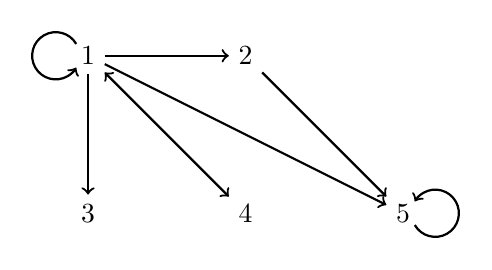
\begin{tikzpicture}
\node (atom1) at (0,2) {1};
\node (atom2) at (2,2) {2};
\node (atom4) at (0,0) {3};
\node (atom5) at (2,0) {4};
\node (atom6) at (4,0) {5};
\draw[->, thick] (atom1)+(-0.15,0.15) arc (-330:-30:.3);
\draw[->, thick] (atom6)+(0.15,-0.15) arc (-150:150:.3);
\draw[->, thick] (atom1) -- (atom2);
\draw[->, thick] (atom1) -- (atom4);
\draw[<->, thick] (atom1) -- (atom5);
\draw[->, thick] (atom1) -- (atom6);
\draw[->, thick] (atom2) -- (atom6);
\end{tikzpicture}
\bmlDescription{Os números 1, 2, 3, 4 e 5 estão conectados por setas.
Há setas de 1 para 2, 3, 4, 5 e para si mesmo; de 2 para 5,
de 5 para si mesmo e de 4 para 1. Não há nenhuma seta saindo de 3.}
\end{center}
Determine se cada uma das seguintes sentenças é verdadeira ou falsa nessa interpretação:
\begin{compactlist}
\item $\exists x\,\atom{R}{x,x}$ \hfill \myanswer{Verdadeiro}
\item $\forall x\,\atom{R}{x,x}$ \hfill \myanswer{Falso}
\item $\exists x \forall y\,\atom{R}{x,y}$ \hfill \myanswer{Verdadeiro}
\item $\exists x \forall y\,\atom{R}{y,x}$ \hfill \myanswer{Falso}
\item $\forall x \forall y \forall z ((\atom{R}{x,y} \eand \atom{R}{y,z}) \eif \atom{R}{x,z})$ \hfill \myanswer{Falso}
\item $\forall x \forall y \forall z ((\atom{R}{x,y} \eand \atom{R}{x,z}) \eif \atom{R}{y,z})$ \hfill \myanswer{Falso}
\item $\exists x \forall y \enot \atom{R}{x,y}$ \hfill \myanswer{Verdadeiro}
\item $\forall x(\exists y\,\atom{R}{x,y} \eif \exists y\,\atom{R}{y,x})$ \hfill \myanswer{Verdadeiro}
\item $\exists x \exists y (\enot x = y \eand \atom{R}{x,y} \eand \atom{R}{y,x})$ \hfill \myanswer{Verdadeiro}
\item $\exists x \forall y(\atom{R}{x,y} \eiff x = y)$ \hfill \myanswer{Verdadeiro}
\item $\exists x \forall y(\atom{R}{y,x} \eiff x = y)$ \hfill \myanswer{Falso}
\item $\exists x \exists y(\enot x = y \eand \atom{R}{x,y} \eand \forall z(\atom{R}{z,x} \eiff y = z))$ \hfill \myanswer{Verdadeiro}
\end{compactlist}

\chapter{Conceitos semânticos}
\setcounter{ProbPart}{0}

\solutions
\problempart
Dada a seguinte interpretação:
\begin{ekey}
	\item[\text{domínio}] pessoas
	\item[\atom{W}{x}] \gap{x} é uma mulher (ou menina)
	\item[\atom{M}{x}] \gap{x} é um homem (ou menino)
	\item[\atom{Y}{x,y}] \gap{x} é mais jovem que \gap{y}
	\item[\atom{O}{x,y}] \gap{x} é descendente de \gap{y}
	\item[d] Dana
	\item[a] Alex
\end{ekey}
expresse as seguintes relações:
\begin{compactlist}
	\item \gap{x} é mais velho que \gap{y} \hfill\myanswer{$\atom{Y}{y,x}$}
	\item \gap{x} é a mãe de \gap{y} \hfill\myanswer{$\atom{O}{y,x}
	\eand \atom{W}{x}$}
	\item \gap{x} e \gap{y} são irmãos (observe que você não pode ser irmão de si mesmo) \hfill\myanswer{$\exists z(\atom{O}{x,z} \eand
	\atom{O}{y,z}) \eand \enot x=y$}

	\item \gap{x} é irmão de \gap{y} \hfill\myanswer{$\exists z(\atom{O}{x,z} \eand
	\atom{O}{y,z}) \eand \enot x=y \eand \atom{M}{x}$}
\end{compactlist}

\problempart
Usando a chave de simbolização do exercício anterior, simbolize as seguintes sentenças:

\begin{compactlist}
	\item Alex e Dana são irmãs. \hfill\myanswer{$\exists z(\atom{O}{a,z} \eand
	\atom{O}{d,z}) \eand \enot a=d \eand \atom{W}{a} \eand \atom{W}{d}$}
	\item Pais são mais velhos que seus filhos.
	\hfill\myanswer{$\forall x\forall y((\atom{O}{x,y} \eand
	\atom{M}{y}) \eif \atom{Y}{x,y})$}
	\item Os pais de Alex têm a mesma idade. \hfill\myanswer{$\forall
	x\forall y((\atom{O}{x,a} \eand
	\atom{O}{y,a}) \eif \enot \atom{Y}{x,y})$}
\end{compactlist}

\chapter{Usando interpretações}\setcounter{ProbPart}{0}

\solutions
\problempart
\label{pr.Contingent}
Mostre que cada uma das seguintes sentenças não é nem uma validade nem uma contradição:
\begin{compactlist}
\item $\atom{D}{a} \eand \atom{D}{b}$

\myanswer{A sentença é verdadeira neste modelo:
\begin{ekey}
	\item[\text{domínio}] Stan
	\item[D(x)] Stan
	\item[a] Stan
	\item[b] Stan
\end{ekey}
E é falsa neste modelo:
\begin{ekey}
	\item[\text{domínio}] Stan
	\item[D(x)] % $\emptyset$
	\item[a] Stan
	\item[b] Stan
\end{ekey}}
\item \leftsolutions\ $\exists x\,\atom{T}{x,h}$

\myanswer{A sentença é verdadeira neste modelo:
\begin{ekey}
	\item[\text{domínio}] Stan
	\item[T(x,y)] \ntuple{Stan, Stan}
	\item[h] Stan
\end{ekey}
E é falsa neste modelo:
\begin{ekey}
	\item[\text{domínio}] Stan
	\item[T(x,y)] % $\emptyset$
	\item[h] Stan
\end{ekey}}

\item $\atom{P}{m} \eand \enot\forall x\,\atom{P}{x}$

\myanswer{	A sentença é verdadeira neste modelo:
\begin{ekey}
	\item[\text{domínio}] Stan, Ollie
	\item[P(x)] Stan
	\item[m] Stan
\end{ekey}
E é falsa neste modelo:
\begin{ekey}
	\item[\text{domínio}] Stan
	\item[P(x)] % $\emptyset$
	\item[m] Stan
\end{ekey}}
\item $\forall z\, \atom{J}{z} \eiff \exists y\,\atom{J}{y}$
\item $\forall x (\atom{W}{x,m,n} \eor \exists y\,\atom{L}{x,y})$
\item $\exists x (\atom{G}{x} \eif \forall y\,\atom{M}{y})$
\item $\exists x (x = h \eand x = i)$
\end{compactlist}

\solutions
\problempart
\label{pr.NotEquiv}
Mostre que os seguintes pares de sentenças não são logicamente equivalentes:
\begin{compactlist}
\item $\atom{J}{a}$, $\atom{K}{a}$

\myanswer{Tornando a primeira sentença verdadeira e a segunda falsa:
\begin{ekey}
	\item[\text{domínio}] $0$
	\item[J(x)] $0$
	\item[K(x)] % $\emptyset$
	\item[a] $0$
\end{ekey}}
\item $\exists x\,\atom{J}{x}$, $\atom{J}{m}$

\myanswer{Tornando a primeira sentença verdadeira e a segunda falsa:
\begin{ekey}
	\item[\text{domínio}] $0$, $1$
	\item[J(x)] $0$
	\item[m] $1$
\end{ekey}}
\item $\forall x\,\atom{R}{x,x}$, $\exists x\,\atom{R}{x,x}$

\myanswer{Tornando a primeira sentença falsa e a segunda verdadeira:
\begin{ekey}
	\item[\text{domínio}] $0$, $1$
	\item[R(x,y)] \ntuple{$0$,$0$}
\end{ekey}}
\item $\exists x\,\atom{P}{x} \eif \atom{Q}{c}$, $\exists x (\atom{P}{x} \eif \atom{Q}{c})$

\myanswer{Tornando a primeira sentença falsa e a segunda verdadeira:
\begin{ekey}
	\item[\text{domínio}] $0$, $1$
	\item[P(x)] $0$
	\item[Q(x)] % $\emptyset$
	\item[c] $0$
\end{ekey}}
\item $\forall x(\atom{P}{x} \eif \enot \atom{Q}{x})$, $\exists x(\atom{P}{x} \eand \enot \atom{Q}{x})$

\myanswer{Tornando a primeira sentença verdadeira e a segunda falsa:
\begin{ekey}
	\item[\text{domínio}] $0$
	\item[P(x)] % $\emptyset$
	\item[Q(x)] % $\emptyset$
\end{ekey}}
\item $\exists x(\atom{P}{x} \eand \atom{Q}{x})$, $\exists x(\atom{P}{x} \eif \atom{Q}{x})$

\myanswer{Tornando a primeira sentença falsa e a segunda verdadeira:
\begin{ekey}
	\item[\text{domínio}] $0$
	\item[P(x)] % $\emptyset$
	\item[Q(x)] $0$
\end{ekey}}
\item $\forall x(\atom{P}{x}\eif \atom{Q}{x})$, $\forall x(\atom{P}{x} \eand \atom{Q}{x})$

\myanswer{Tornando a primeira sentença verdadeira e a segunda falsa:
\begin{ekey}
	\item[\text{domínio}] $0$
	\item[P(x)] % $\emptyset$
	\item[Q(x)] $0$
\end{ekey}}
\item $\forall x\exists y\,\atom{R}{x,y}$, $\exists x\forall y\,\atom{R}{x,y}$

\myanswer{Tornando a primeira sentença verdadeira e a segunda falsa:
\begin{ekey}
	\item[\text{domínio}] $0$, $1$
	\item[R(x,y)] \ntuple{$0$, $1$}, \ntuple{$1$, $0$}
\end{ekey}}
\item $\forall x\exists y\,\atom{R}{x,y}$, $\forall x\exists y\,\atom{R}{y,x}$

\myanswer{Tornando a primeira sentença falsa e a segunda verdadeira:
\begin{ekey}
	\item[\text{domínio}] $0$, $1$
	\item[R(x,y)] \ntuple{$0$, $0$}, \ntuple{$0$, $1$}
\end{ekey}}
\end{compactlist}


\problempart
Mostre que as seguintes sentenças são conjuntamente satisfatíveis:
\begin{compactlist}
\item $\atom{M}{a}, \enot \atom{N}{a}, Pa, \enot \atom{Q}{a}$
\item $\atom{L}{e,e}, \atom{L}{e,g}, \enot \atom{L}{g,e}, \enot \atom{L}{g,g}$
\item $\enot (\atom{M}{a} \eand \exists x\,\atom{A}{x}), Ma \eor \atom{F}{a}, \forall x(\atom{F}{x} \eif \atom{A}{x})$
\item $\atom{M}{a} \eor \atom{M}{b}, \atom{M}{a} \eif \forall x \enot \atom{M}{x}$
\item $\forall y\,\atom{G}{y}, \forall x (\atom{G}{x} \eif \atom{H}{x}), \exists y \enot \atom{I}{y}$
\item $\exists x(\atom{B}{x} \eor \atom{A}{x}), \forall x \enot \atom{C}{x}, \forall x\bigl[(\atom{A}{x} \eand \atom{B}{x}) \eif \atom{C}{x}\bigr]$
\item $\exists x\,\atom{X}{x}, \exists x\,\atom{Y}{x}, \forall x(\atom{X}{x} \eiff \enot \atom{Y}{x})$
\item $\forall x(\atom{P}{x} \eor \atom{Q}{x}), \exists x\enot(\atom{Q}{x} \eand \atom{P}{x})$
\item $\exists z(\atom{N}{z} \eand \atom{O}{z,z}), \forall x\forall y(\atom{O}{x,y} \eif \atom{O}{y,x})$
\item $\enot \exists x \forall y\,\atom{R}{x,y}, \forall x \exists y\,\atom{R}{x,y}$
\item $\enot \atom{R}{a,a}$, $\forall x (x=a \eor \atom{R}{x,a})$

\myanswer{As sentenças são ambas verdadeiras nesta interpretação:
\begin{ekey}
	\item[\text{domínio}] Harry, Sally
	\item[R(x,y)]\ntuple{Sally, Harry}
	\item[a] Harry
	\end{ekey}}
\item $\forall x\forall y\forall z[(x=y \eor y=z )\eor x=z]$, $\exists x\exists y\ \enot x= y$

\myanswer{Não há predicados nem constantes, portanto só precisamos fornecer um domínio. Qualquer domínio com 2 elementos servirá.}

\item $\exists x\exists y((\atom{Z}{x} \eand \atom{Z}{y} )\eand x=y)$, $\enot \atom{Z}{d}$, $d=e$
\end{compactlist}

\problempart
Mostre que os seguintes argumentos são inválidos:
\begin{compactlist}
\item $\forall x(\atom{A}{x} \eif \atom{B}{x}) \therefore \exists x\,\atom{B}{x}$
\item $\forall x(\atom{R}{x} \eif \atom{D}{x}), \forall x(\atom{R}{x} \eif \atom{F}{x}) \therefore \exists x(\atom{D}{x} \eand \atom{F}{x})$
\item $\exists x(\atom{P}{x}\eif \atom{Q}{x}) \therefore \exists x\,\atom{P}{x}$
\item $\atom{N}{a} \eand \atom{N}{b} \eand \atom{N}{c} \therefore \forall x\,\atom{N}{x}$
\item $\atom{R}{d,e}, \exists x\,\atom{R}{xd} \therefore \atom{R}{e,d}$
\item $\exists x(\atom{E}{x} \eand \atom{F}{x}), \exists x\,\atom{F}{x} \eif \exists x\,\atom{G}{x} \therefore \exists x(\atom{E}{x} \eand \atom{G}{x})$
\item $\forall x\,\atom{O}{x,c}, \forall x\,\atom{O}{c,x} \therefore \forall x\,\atom{O}{x,x}$
\item $\exists x(\atom{J}{x} \eand \atom{K}{x}), \exists x \enot \atom{K}{x}, \exists x \enot \atom{J}{x} \therefore \exists x(\enot \atom{J}{x} \eand \enot \atom{K}{x})$
\item $\atom{L}{a,b} \eif \forall x\,\atom{L}{x,b}, \exists x\,\atom{L}{x,b} \therefore \atom{L}{b,b}$
\item $\forall x(\atom{D}{x} \eif \exists y\,\atom{T}{y,x}) \therefore \exists y \exists z\ \enot y= z$
\end{compactlist}

\stepcounter{chapter} % Reasoning about interpretations

\chapter{Propriedades das relações}
\setcounter{ProbPart}{0}

\solutions
\problempart
Dê exemplos de relações com as seguintes propriedades:
\begin{compactlist}
	\item Reflexiva, mas não simétrica \hfill\myanswer{\gap{x} não é mais velho que \gap{y}}

	\item Simétrica, mas não transitiva \hfill\myanswer{\gap{x} está a menos de 1~km de \gap{y}}

	\item Transitiva, simétrica, mas não reflexiva
	\hfill\myanswer{\gap{x} é irmão ou irmã pleno (isto é, não meio-irmão) de \gap{y}}
\end{compactlist}

\problempart
Mostre que uma relação pode ser simultaneamente simétrica e antissimétrica, fornecendo uma interpretação que torne verdadeiras as duas sentenças seguintes:


\begin{align*}
	& \forall x\forall y(\atom{R}{x,y} \eif \atom{R}{y,x})\\
	& \forall x\forall y((\atom{R}{x,y} \eand \atom{R}{y,x}) \eif x=y)
\end{align*}
\myanswer{\begin{ekey}
	\item[\text{domínio}] $0$
	\item[\atom{R}{x,y}] \ntuple{$0$, $0$}
\end{ekey}}

\input{solutions/forallx-sol-prooffol}
\input{solutions/forallx-sol-ml}

\chapter{Formas normais}\setcounter{ProbPart}{0}

\problempart
\label{pr.DNF}
Considere as seguintes sentenças:
	\begin{compactlist}
		\item $(A \eif \enot B)$
		\item $\enot (A \eiff B)$
		\item $(\enot A \eor \enot (A \eand B))$
		\item $(\enot (A \eif B ) \eand (A \eif C))$
		\item $(\enot (A \eor B) \eiff ((\enot C \eand \enot A) \eif \enot B))$
		\item $((\enot (A \eand \enot B) \eif C) \eand \enot (A \eand D))$
	\end{compactlist}
Para cada sentença, encontre uma sentença equivalente na FND e outra na FNC.
\myanswer{Daremos uma solução para (2). A tabela-verdade de $\enot (A \eiff B)$ é:
\begin{center}
\begin{tabular}{c c | l}
$A$ & $B$ & $\enot (A \eiff B)$\\
\hline
T & T & F \\
T & F & T \\
F & T & T \\
F & F & F \\
\end{tabular}
\end{center}
Uma sentença na FND pode ser lida nas linhas 2 e 3:
\[(A \eand \enot B) \eor (\enot A \eand B)\]
e uma na FNC nas linhas 1 e~4:
\[(\enot A \eor \enot B) \eand (A \eor B).\]}

\stepcounter{chapter} % Functional completeness

\chapter{Demonstração de equivalências}\setcounter{ProbPart}{0}

\problempart
\label{pr.DNF2}
Considere as seguintes sentenças:
\begin{compactlist}
	\item $(A \eif \enot B)$
	\item $\enot (A \eiff B)$
	\item $(\enot A \eor \enot (A \eand B))$
	\item $(\enot (A \eif B ) \eand (A \eif C))$
	\item $(\enot (A \eor B) \eiff ((\enot C \eand \enot A) \eif \enot B))$
	\item $((\enot (A \eand \enot B) \eif C) \eand \enot (A \eand D))$
\end{compactlist}
Para cada sentença, encontre uma sentença equivalente na FND e outra na FNC fornecendo uma cadeia de equivalências. Use (Id), (Absorp) e (Simp) para simplificar suas sentenças tanto quanto possível.
\myanswer{Daremos uma solução para (2). Remover $\eiff$ e empurrar as negações para dentro é comum a ambas:
\begin{align*}
	& \enot (A \eiff B)\\
	& \enot((A \eif B) \eand (B \eif A)) && \text{Bicond}\\
	& \enot((\enot A \eor B) \eand (B \eif A)) && \text{Cond}\\
	& \enot((\enot A \eor B) \eand (\enot B \eor A)) && \text{Cond}\\
	& \enot(\enot A \eor B) \eor \enot(\enot B \eor A) && \text{DeM}\\
	& (\enot\enot A \eand \enot B) \eor (\enot\enot B \eand \enot A) && \text{DeM}\\
	& (A \eand \enot B) \eor (\enot\enot B \eand \enot A) && \text{DN}\\
	& (A \eand \enot B) \eor (B \eand \enot A) && \text{DN}
\intertext{O resultado está agora na FND. Para obter uma FNC, continuamos usando (Comm) e (Dist):}
& ((A \eand \enot B) \eor B) \eand ((A \eand \enot B) \eor \enot A) && \text{Dist}\\
& (B \eor (A \eand \enot B)) \eand ((A \eand \enot B) \eor \enot A) && \text{Comm}\\
& ((B \eor A) \eand (B \eor \enot B)) \eand ((A \eand \enot B) \eor \enot A) && \text{Dist}\\
& ((B \eor A) \eand (B \eor \enot B)) \eand (\enot A \eor (A \eand \enot B)) && \text{Comm}\\
& ((B \eor A) \eand (B \eor \enot B)) \eand ((\enot A \eor A) \eand (\enot A \eor \enot B)) && \text{Dist}\\
\intertext{O resultado pode ser simplificado usando (Simp):}
& (B \eor A) \eand ((\enot A \eor A) \eand (\enot A \eor \enot B)) && \text{Simp}\\
& (B \eor A) \eand (\enot A \eor \enot B) && \text{Simp}
\end{align*}}

\stepcounter{chapter} % Soundness
\end{document}
